\documentclass[twoside]{book}

% Packages required by doxygen
\usepackage{fixltx2e}
\usepackage{calc}
\usepackage{doxygen}
\usepackage[export]{adjustbox} % also loads graphicx
\usepackage{graphicx}
\usepackage[utf8]{inputenc}
\usepackage{makeidx}
\usepackage{multicol}
\usepackage{multirow}
\PassOptionsToPackage{warn}{textcomp}
\usepackage{textcomp}
\usepackage[nointegrals]{wasysym}
\usepackage[table]{xcolor}

% Font selection
\usepackage[T1]{fontenc}
\usepackage[scaled=.90]{helvet}
\usepackage{courier}
\usepackage{amssymb}
\usepackage{sectsty}
\renewcommand{\familydefault}{\sfdefault}
\allsectionsfont{%
  \fontseries{bc}\selectfont%
  \color{darkgray}%
}
\renewcommand{\DoxyLabelFont}{%
  \fontseries{bc}\selectfont%
  \color{darkgray}%
}
\newcommand{\+}{\discretionary{\mbox{\scriptsize$\hookleftarrow$}}{}{}}

% Page & text layout
\usepackage{geometry}
\geometry{%
  a4paper,%
  top=2.5cm,%
  bottom=2.5cm,%
  left=2.5cm,%
  right=2.5cm%
}
\tolerance=750
\hfuzz=15pt
\hbadness=750
\setlength{\emergencystretch}{15pt}
\setlength{\parindent}{0cm}
\setlength{\parskip}{3ex plus 2ex minus 2ex}
\makeatletter
\renewcommand{\paragraph}{%
  \@startsection{paragraph}{4}{0ex}{-1.0ex}{1.0ex}{%
    \normalfont\normalsize\bfseries\SS@parafont%
  }%
}
\renewcommand{\subparagraph}{%
  \@startsection{subparagraph}{5}{0ex}{-1.0ex}{1.0ex}{%
    \normalfont\normalsize\bfseries\SS@subparafont%
  }%
}
\makeatother

% Headers & footers
\usepackage{fancyhdr}
\pagestyle{fancyplain}
\fancyhead[LE]{\fancyplain{}{\bfseries\thepage}}
\fancyhead[CE]{\fancyplain{}{}}
\fancyhead[RE]{\fancyplain{}{\bfseries\leftmark}}
\fancyhead[LO]{\fancyplain{}{\bfseries\rightmark}}
\fancyhead[CO]{\fancyplain{}{}}
\fancyhead[RO]{\fancyplain{}{\bfseries\thepage}}
\fancyfoot[LE]{\fancyplain{}{}}
\fancyfoot[CE]{\fancyplain{}{}}
\fancyfoot[RE]{\fancyplain{}{\bfseries\scriptsize Generated by Doxygen }}
\fancyfoot[LO]{\fancyplain{}{\bfseries\scriptsize Generated by Doxygen }}
\fancyfoot[CO]{\fancyplain{}{}}
\fancyfoot[RO]{\fancyplain{}{}}
\renewcommand{\footrulewidth}{0.4pt}
\renewcommand{\chaptermark}[1]{%
  \markboth{#1}{}%
}
\renewcommand{\sectionmark}[1]{%
  \markright{\thesection\ #1}%
}

% Indices & bibliography
\usepackage{natbib}
\usepackage[titles]{tocloft}
\setcounter{tocdepth}{3}
\setcounter{secnumdepth}{5}
\makeindex

% Hyperlinks (required, but should be loaded last)
\usepackage{ifpdf}
\ifpdf
  \usepackage[pdftex,pagebackref=true]{hyperref}
\else
  \usepackage[ps2pdf,pagebackref=true]{hyperref}
\fi
\hypersetup{%
  colorlinks=true,%
  linkcolor=blue,%
  citecolor=blue,%
  unicode%
}

% Custom commands
\newcommand{\clearemptydoublepage}{%
  \newpage{\pagestyle{empty}\cleardoublepage}%
}

\usepackage{caption}
\captionsetup{labelsep=space,justification=centering,font={bf},singlelinecheck=off,skip=4pt,position=top}

%===== C O N T E N T S =====

\begin{document}

% Titlepage & ToC
\hypersetup{pageanchor=false,
             bookmarksnumbered=true,
             pdfencoding=unicode
            }
\pagenumbering{alph}
\begin{titlepage}
\vspace*{7cm}
\begin{center}%
{\Large dimension/dimension/dimension }\\
\vspace*{1cm}
{\large Generated by Doxygen 1.8.13}\\
\end{center}
\end{titlepage}
\clearemptydoublepage
\pagenumbering{roman}
\tableofcontents
\clearemptydoublepage
\pagenumbering{arabic}
\hypersetup{pageanchor=true}

%--- Begin generated contents ---
\chapter{Namespace Index}
\section{Namespace List}
Here is a list of all documented namespaces with brief descriptions\+:\begin{DoxyCompactList}
\item\contentsline{section}{\hyperlink{namespaceacme}{acme} }{\pageref{namespaceacme}}{}
\end{DoxyCompactList}

\chapter{Class Index}
\section{Class List}
Here are the classes, structs, unions and interfaces with brief descriptions\+:\begin{DoxyCompactList}
\item\contentsline{section}{\hyperlink{classddd_1_1box}{ddd\+::box$<$ T $>$} \\*Box class container }{\pageref{classddd_1_1box}}{}
\item\contentsline{section}{\hyperlink{classddd_1_1circle}{ddd\+::circle$<$ T $>$} }{\pageref{classddd_1_1circle}}{}
\item\contentsline{section}{\hyperlink{classddd_1_1coord}{ddd\+::coord$<$ T $>$} }{\pageref{classddd_1_1coord}}{}
\item\contentsline{section}{\hyperlink{classddd_1_1line}{ddd\+::line$<$ T $>$} \\*Line class container }{\pageref{classddd_1_1line}}{}
\item\contentsline{section}{\hyperlink{classddd_1_1plane}{ddd\+::plane$<$ T $>$} \\*Plane class container }{\pageref{classddd_1_1plane}}{}
\item\contentsline{section}{\hyperlink{classddd_1_1point}{ddd\+::point$<$ T $>$} \\*Point class container }{\pageref{classddd_1_1point}}{}
\item\contentsline{section}{\hyperlink{classddd_1_1quadix}{ddd\+::quadix$<$ T $>$} \\*Quadix class container }{\pageref{classddd_1_1quadix}}{}
\item\contentsline{section}{\hyperlink{classddd_1_1ray}{ddd\+::ray$<$ T $>$} \\*Ray class container }{\pageref{classddd_1_1ray}}{}
\item\contentsline{section}{\hyperlink{classddd_1_1rotation}{ddd\+::rotation$<$ T $>$} \\*Rotation class container }{\pageref{classddd_1_1rotation}}{}
\item\contentsline{section}{\hyperlink{classddd_1_1segment}{ddd\+::segment$<$ T $>$} \\*Segment class container }{\pageref{classddd_1_1segment}}{}
\item\contentsline{section}{\hyperlink{classddd_1_1sphere}{ddd\+::sphere$<$ T $>$} \\*Sphere class container }{\pageref{classddd_1_1sphere}}{}
\item\contentsline{section}{\hyperlink{class_tic_toc}{Tic\+Toc} }{\pageref{class_tic_toc}}{}
\item\contentsline{section}{\hyperlink{classddd_1_1triangle}{ddd\+::triangle$<$ T $>$} \\*Triangle class container }{\pageref{classddd_1_1triangle}}{}
\item\contentsline{section}{\hyperlink{classddd_1_1vector}{ddd\+::vector$<$ T $>$} \\*Vector class container }{\pageref{classddd_1_1vector}}{}
\end{DoxyCompactList}

\chapter{Namespace Documentation}
\hypertarget{namespaceddd}{}\section{ddd Namespace Reference}
\label{namespaceddd}\index{ddd@{ddd}}
\subsection*{Classes}
\begin{DoxyCompactItemize}
\item 
class \hyperlink{classddd_1_1box}{box}
\begin{DoxyCompactList}\small\item\em Box class container. \end{DoxyCompactList}\item 
class \hyperlink{classddd_1_1circle}{circle}
\item 
class \hyperlink{classddd_1_1coord}{coord}
\item 
class \hyperlink{classddd_1_1line}{line}
\begin{DoxyCompactList}\small\item\em Line class container. \end{DoxyCompactList}\item 
class \hyperlink{classddd_1_1plane}{plane}
\begin{DoxyCompactList}\small\item\em Plane class container. \end{DoxyCompactList}\item 
class \hyperlink{classddd_1_1point}{point}
\begin{DoxyCompactList}\small\item\em Point class container. \end{DoxyCompactList}\item 
class \hyperlink{classddd_1_1quadix}{quadix}
\begin{DoxyCompactList}\small\item\em Quadix class container. \end{DoxyCompactList}\item 
class \hyperlink{classddd_1_1ray}{ray}
\begin{DoxyCompactList}\small\item\em Ray class container. \end{DoxyCompactList}\item 
class \hyperlink{classddd_1_1rotation}{rotation}
\begin{DoxyCompactList}\small\item\em Rotation class container. \end{DoxyCompactList}\item 
class \hyperlink{classddd_1_1segment}{segment}
\begin{DoxyCompactList}\small\item\em Segment class container. \end{DoxyCompactList}\item 
class \hyperlink{classddd_1_1sphere}{sphere}
\begin{DoxyCompactList}\small\item\em Sphere class container. \end{DoxyCompactList}\item 
class \hyperlink{classddd_1_1triangle}{triangle}
\begin{DoxyCompactList}\small\item\em Triangle class container. \end{DoxyCompactList}\item 
class \hyperlink{classddd_1_1vector}{vector}
\begin{DoxyCompactList}\small\item\em Vector class container. \end{DoxyCompactList}\end{DoxyCompactItemize}
\subsection*{Typedefs}
\begin{DoxyCompactItemize}
\item 
\mbox{\Hypertarget{namespaceddd_a900cde04ff126705e451a03e280e1c7a}\label{namespaceddd_a900cde04ff126705e451a03e280e1c7a}} 
typedef double \hyperlink{namespaceddd_a900cde04ff126705e451a03e280e1c7a}{Float}
\begin{DoxyCompactList}\small\item\em Real number type. \end{DoxyCompactList}\item 
\mbox{\Hypertarget{namespaceddd_a50ea76e2b817cc6c6b4539c7f3c4bdad}\label{namespaceddd_a50ea76e2b817cc6c6b4539c7f3c4bdad}} 
typedef int \hyperlink{namespaceddd_a50ea76e2b817cc6c6b4539c7f3c4bdad}{Int}
\begin{DoxyCompactList}\small\item\em Integer number type. \end{DoxyCompactList}\end{DoxyCompactItemize}
\subsection*{Functions}
\begin{DoxyCompactItemize}
\item 
\mbox{\Hypertarget{namespaceddd_ad85f2129847410744f5a20fe364c11b1}\label{namespaceddd_ad85f2129847410744f5a20fe364c11b1}} 
{\footnotesize template$<$typename T $>$ }\\T \hyperlink{namespaceddd_ad85f2129847410744f5a20fe364c11b1}{infinity} ()
\begin{DoxyCompactList}\small\item\em Return infinity value. \end{DoxyCompactList}\item 
\mbox{\Hypertarget{namespaceddd_ab55dae45d0811c0c1bf70ac26ddd9a31}\label{namespaceddd_ab55dae45d0811c0c1bf70ac26ddd9a31}} 
{\footnotesize template$<$typename T $>$ }\\T \hyperlink{namespaceddd_ab55dae45d0811c0c1bf70ac26ddd9a31}{epsilon} ()
\begin{DoxyCompactList}\small\item\em Return epsilon value. \end{DoxyCompactList}\item 
\mbox{\Hypertarget{namespaceddd_a1a221e63a5d10669dcd87178911cdac5}\label{namespaceddd_a1a221e63a5d10669dcd87178911cdac5}} 
{\footnotesize template$<$$>$ }\\double \hyperlink{namespaceddd_a1a221e63a5d10669dcd87178911cdac5}{epsilon$<$ double $>$} ()
\begin{DoxyCompactList}\small\item\em Return specific double-\/type epsilon value. \end{DoxyCompactList}\item 
\mbox{\Hypertarget{namespaceddd_a19135a4582ea8e38ebb186e9dfd75eb8}\label{namespaceddd_a19135a4582ea8e38ebb186e9dfd75eb8}} 
{\footnotesize template$<$$>$ }\\float \hyperlink{namespaceddd_a19135a4582ea8e38ebb186e9dfd75eb8}{epsilon$<$ float $>$} ()
\begin{DoxyCompactList}\small\item\em Return specific float-\/type epsilon value. \end{DoxyCompactList}\item 
{\footnotesize template$<$typename T $>$ }\\T \hyperlink{namespaceddd_a1d4703ab7fa9c58943ff44b368dacb4b}{sqr} (const T \&value)
\begin{DoxyCompactList}\small\item\em Square function. \end{DoxyCompactList}\item 
{\footnotesize template$<$typename T $>$ }\\T \hyperlink{namespaceddd_abbdb4782fa0a78950fd49de0d5766dd2}{cub} (const T \&value)
\begin{DoxyCompactList}\small\item\em Cubic function. \end{DoxyCompactList}\item 
{\footnotesize template$<$typename T $>$ }\\T \hyperlink{namespaceddd_a99ebeda8499ba29e0302f0f3c6e43549}{sqrt} (const T \&value)
\begin{DoxyCompactList}\small\item\em Square root function. \end{DoxyCompactList}\item 
{\footnotesize template$<$typename T $>$ }\\T \hyperlink{namespaceddd_a9ac20d4240d0a9fa208e3dd220101a0a}{abs} (const T \&value)
\begin{DoxyCompactList}\small\item\em Absolute value function. \end{DoxyCompactList}\item 
{\footnotesize template$<$typename T $>$ }\\T \hyperlink{namespaceddd_ac22862b5ed1b5bf5ba4d52e4a740bef9}{max} (const T \&value0, const T \&value1)
\begin{DoxyCompactList}\small\item\em Maximum between two values function. \end{DoxyCompactList}\item 
{\footnotesize template$<$typename T $>$ }\\T \hyperlink{namespaceddd_aa11a0222d3d3c7580e0b8b40b38258df}{min} (const T \&value0, const T \&value1)
\begin{DoxyCompactList}\small\item\em Minimum between two values function. \end{DoxyCompactList}\item 
{\footnotesize template$<$typename T $>$ }\\T \hyperlink{namespaceddd_a64cb844784cf8f7a2a9d691f7c6bcba3}{max} (const T \&value0, const T \&value1, const T \&value2)
\begin{DoxyCompactList}\small\item\em Maximum between three values function. \end{DoxyCompactList}\item 
{\footnotesize template$<$typename T $>$ }\\T \hyperlink{namespaceddd_a563d604cd5ed6ee708fffa32cbe6ccf2}{min} (const T \&value0, const T \&value1, const T \&value2)
\begin{DoxyCompactList}\small\item\em Minimum between three values function. \end{DoxyCompactList}\item 
{\footnotesize template$<$typename T $>$ }\\T \hyperlink{namespaceddd_a3c2355d52318b82d63a4ff3525bb651a}{sin} (const T \&value)
\begin{DoxyCompactList}\small\item\em Sine function \mbox{[}rad\mbox{]}. \end{DoxyCompactList}\item 
{\footnotesize template$<$typename T $>$ }\\T \hyperlink{namespaceddd_a6a7f708bb835a257f25e87110af27b6a}{cos} (const T \&value)
\begin{DoxyCompactList}\small\item\em Cosine function \mbox{[}rad\mbox{]}. \end{DoxyCompactList}\item 
{\footnotesize template$<$typename T $>$ }\\T \hyperlink{namespaceddd_aeb0ca0d620545cbb5ef955eed88d1c0d}{tan} (const T \&value)
\begin{DoxyCompactList}\small\item\em Tangent function \mbox{[}rad\mbox{]}. \end{DoxyCompactList}\item 
{\footnotesize template$<$typename T $>$ }\\T \hyperlink{namespaceddd_af887d6f09da2128f99b36b034ab2ed1f}{asin} (const T \&value)
\begin{DoxyCompactList}\small\item\em Arcsine function \mbox{[}rad\mbox{]}. \end{DoxyCompactList}\item 
{\footnotesize template$<$typename T $>$ }\\T \hyperlink{namespaceddd_a03e440b351f44fec5abac1270231e3bb}{acos} (const T \&value)
\begin{DoxyCompactList}\small\item\em Arccosine function \mbox{[}rad\mbox{]}. \end{DoxyCompactList}\item 
{\footnotesize template$<$typename T $>$ }\\T \hyperlink{namespaceddd_a750f7cad6893bbbfbaa51353044bde4f}{atan} (const T \&value)
\begin{DoxyCompactList}\small\item\em Arctangent function \mbox{[}rad\mbox{]}. \end{DoxyCompactList}\item 
{\footnotesize template$<$typename T $>$ }\\T \hyperlink{namespaceddd_a1dea631509d981c3718796774b796d6c}{atan2} (const T \&value0, const T \&value1)
\begin{DoxyCompactList}\small\item\em Arctangent function \mbox{[}rad\mbox{]}. \end{DoxyCompactList}\item 
{\footnotesize template$<$typename T $>$ }\\T \hyperlink{namespaceddd_a070060e53a22cb16f07576bfb5c4b1cc}{clamp} (const T \&value, const T \&low, const T \&high)
\begin{DoxyCompactList}\small\item\em Clamp function (returns the input value bounded between low and high values) \end{DoxyCompactList}\item 
{\footnotesize template$<$typename T $>$ }\\T \hyperlink{namespaceddd_a7d68733d32a94776596a8e213ae9fcdf}{is\+\_\+equal} (const T \&value0, const T \&value1, const T \&tolerance=Epsilon\+\_\+\+High)
\begin{DoxyCompactList}\small\item\em Check if two elements are almost equal. \end{DoxyCompactList}\item 
{\footnotesize template$<$typename T $>$ }\\T \hyperlink{namespaceddd_a9b12e82fa10b6beadb08360007e6b57b}{is\+\_\+notequal} (const T \&value0, const T \&value1, const T \&tolerance=Epsilon\+\_\+\+High)
\begin{DoxyCompactList}\small\item\em Check if two elements are N\+OT almost equal. \end{DoxyCompactList}\item 
{\footnotesize template$<$typename T $>$ }\\Eigen\+::\+Matrix$<$ T, 3, 3 $>$ \hyperlink{namespaceddd_ad45c0a592c1aebe03fc48a0c57d52641}{rotate\+\_\+x} (const T \&input)
\begin{DoxyCompactList}\small\item\em Get rotation on x-\/axis. \end{DoxyCompactList}\item 
{\footnotesize template$<$typename T $>$ }\\Eigen\+::\+Matrix$<$ T, 3, 3 $>$ \hyperlink{namespaceddd_a91c74ff16a602f1f611759e2e9f594f3}{rotate\+\_\+y} (const T \&input)
\begin{DoxyCompactList}\small\item\em Get rotation on y-\/axis. \end{DoxyCompactList}\item 
{\footnotesize template$<$typename T $>$ }\\Eigen\+::\+Matrix$<$ T, 3, 3 $>$ \hyperlink{namespaceddd_a8b9d6f84cbf4f443881fd3b3abad07e4}{rotate\+\_\+z} (const T \&input)
\begin{DoxyCompactList}\small\item\em Get rotation on z-\/axis. \end{DoxyCompactList}\item 
\mbox{\Hypertarget{namespaceddd_ae7562b0e49ae64d1740ac6f68f81fdef}\label{namespaceddd_ae7562b0e49ae64d1740ac6f68f81fdef}} 
{\footnotesize template$<$typename T $>$ }\\const Eigen\+::\+Matrix$<$ T, 3, 3 $>$ \& {\bfseries rotation\+\_\+x} (const T \&input)
\item 
\mbox{\Hypertarget{namespaceddd_a99646f415772db90f4df4fb5dd4d458d}\label{namespaceddd_a99646f415772db90f4df4fb5dd4d458d}} 
{\footnotesize template$<$typename T $>$ }\\const Eigen\+::\+Matrix$<$ T, 3, 3 $>$ \& {\bfseries rotation\+\_\+y} (const T \&input)
\item 
\mbox{\Hypertarget{namespaceddd_a03a4cb214ac10e4199f9cbe342cf68f6}\label{namespaceddd_a03a4cb214ac10e4199f9cbe342cf68f6}} 
{\footnotesize template$<$typename T $>$ }\\const Eigen\+::\+Matrix$<$ T, 3, 3 $>$ \& {\bfseries rotation\+\_\+z} (const T \&input)
\item 
{\footnotesize template$<$typename T $>$ }\\std\+::ostream \& \hyperlink{namespaceddd_a02d73e2ba5a018e4e525deb8aea3c0a8}{operator$<$$<$} (std\+::ostream \&os, const \hyperlink{classddd_1_1point}{point}$<$ T $>$ \&obj)
\begin{DoxyCompactList}\small\item\em $<$ Stream out operator for point object \end{DoxyCompactList}\item 
{\footnotesize template$<$typename T $>$ }\\std\+::ostream \& \hyperlink{namespaceddd_a85783ffbd6985b1981059732d7bbe174}{operator$<$$<$} (std\+::ostream \&os, const \hyperlink{classddd_1_1vector}{vector}$<$ T $>$ \&obj)
\begin{DoxyCompactList}\small\item\em Stream out operator for line object. \end{DoxyCompactList}\item 
{\footnotesize template$<$typename T $>$ }\\std\+::ostream \& \hyperlink{namespaceddd_a2001eec5d960802592e1ca6a5b0dc203}{operator$<$$<$} (std\+::ostream \&os, const \hyperlink{classddd_1_1line}{line}$<$ T $>$ \&obj)
\begin{DoxyCompactList}\small\item\em Stream out operator for ray object. \end{DoxyCompactList}\item 
{\footnotesize template$<$typename T $>$ }\\std\+::ostream \& \hyperlink{namespaceddd_ae2604d6c72853dfb2595f6882cbc7a51}{operator$<$$<$} (std\+::ostream \&os, const \hyperlink{classddd_1_1ray}{ray}$<$ T $>$ \&obj)
\begin{DoxyCompactList}\small\item\em Stream out operator. \end{DoxyCompactList}\item 
{\footnotesize template$<$typename T $>$ }\\std\+::ostream \& \hyperlink{namespaceddd_af1faa02295670c7cfd7f0278e3973f84}{operator$<$$<$} (std\+::ostream \&os, const \hyperlink{classddd_1_1plane}{plane}$<$ T $>$ \&obj)
\begin{DoxyCompactList}\small\item\em Stream out operator for segment object. \end{DoxyCompactList}\item 
{\footnotesize template$<$typename T $>$ }\\std\+::ostream \& \hyperlink{namespaceddd_a59e2fa950fd945aa8b3dd550720ad3f5}{operator$<$$<$} (std\+::ostream \&os, const \hyperlink{classddd_1_1segment}{segment}$<$ T $>$ \&obj)
\begin{DoxyCompactList}\small\item\em Stream out operator for box object. \end{DoxyCompactList}\item 
{\footnotesize template$<$typename T $>$ }\\std\+::ostream \& \hyperlink{namespaceddd_af710b0f11be50190553c743ce86545a3}{operator$<$$<$} (std\+::ostream \&os, const \hyperlink{classddd_1_1box}{box}$<$ T $>$ \&obj)
\begin{DoxyCompactList}\small\item\em Stream out operator for triangle object. \end{DoxyCompactList}\item 
{\footnotesize template$<$typename T $>$ }\\std\+::ostream \& \hyperlink{namespaceddd_a3a6f828f85e4fa306f0d950f1aab4f64}{operator$<$$<$} (std\+::ostream \&os, const \hyperlink{classddd_1_1triangle}{triangle}$<$ T $>$ \&obj)
\begin{DoxyCompactList}\small\item\em Stream out operator. \end{DoxyCompactList}\item 
{\footnotesize template$<$typename T $>$ }\\std\+::ostream \& \hyperlink{namespaceddd_a58ae88cefdf3b919e400db6de59f4cfc}{operator$<$$<$} (std\+::ostream \&os, const \hyperlink{classddd_1_1quadix}{quadix}$<$ T $>$ \&obj)
\item 
{\footnotesize template$<$typename T $>$ }\\std\+::ostream \& \hyperlink{namespaceddd_a64dbb41c0ee377eb528907f3448514f6}{operator$<$$<$} (std\+::ostream \&os, const \hyperlink{classddd_1_1sphere}{sphere}$<$ T $>$ \&obj)
\begin{DoxyCompactList}\small\item\em $<$ Stream out operator \end{DoxyCompactList}\end{DoxyCompactItemize}


\subsection{Detailed Description}
file\+: ddd.\+cc

file\+: \hyperlink{ddd_8hh_source}{ddd.\+hh}

file\+: \hyperlink{ddd__box_8hh_source}{ddd\+\_\+box.\+hh}

file\+: ddd\+\_\+sphere.\+hh

file\+: \hyperlink{ddd__instantiate_8hh_source}{ddd\+\_\+instantiate.\+hh}

file\+: \hyperlink{ddd__line_8hh_source}{ddd\+\_\+line.\+hh}

file\+: \hyperlink{ddd__plane_8hh_source}{ddd\+\_\+plane.\+hh}

file\+: \hyperlink{ddd__point_8hh_source}{ddd\+\_\+point.\+hh}

file\+: \hyperlink{ddd__quadix_8hh_source}{ddd\+\_\+quadix.\+hh}

file\+: \hyperlink{ddd__ray_8hh_source}{ddd\+\_\+ray.\+hh}

file\+: \hyperlink{ddd__rotation_8hh_source}{ddd\+\_\+rotation.\+hh}

file\+: \hyperlink{ddd__segment_8hh_source}{ddd\+\_\+segment.\+hh}

file\+: \hyperlink{ddd__triangle_8hh_source}{ddd\+\_\+triangle.\+hh} 

\subsection{Function Documentation}
\mbox{\Hypertarget{namespaceddd_a9ac20d4240d0a9fa208e3dd220101a0a}\label{namespaceddd_a9ac20d4240d0a9fa208e3dd220101a0a}} 
\index{ddd@{ddd}!abs@{abs}}
\index{abs@{abs}!ddd@{ddd}}
\subsubsection{\texorpdfstring{abs()}{abs()}}
{\footnotesize\ttfamily template$<$typename T $>$ \\
T ddd\+::abs (\begin{DoxyParamCaption}\item[{const T \&}]{value }\end{DoxyParamCaption})\hspace{0.3cm}{\ttfamily [inline]}}



Absolute value function. 


\begin{DoxyParams}{Parameters}
{\em value} & Input value \\
\hline
\end{DoxyParams}
\mbox{\Hypertarget{namespaceddd_a03e440b351f44fec5abac1270231e3bb}\label{namespaceddd_a03e440b351f44fec5abac1270231e3bb}} 
\index{ddd@{ddd}!acos@{acos}}
\index{acos@{acos}!ddd@{ddd}}
\subsubsection{\texorpdfstring{acos()}{acos()}}
{\footnotesize\ttfamily template$<$typename T $>$ \\
T ddd\+::acos (\begin{DoxyParamCaption}\item[{const T \&}]{value }\end{DoxyParamCaption})\hspace{0.3cm}{\ttfamily [inline]}}



Arccosine function \mbox{[}rad\mbox{]}. 


\begin{DoxyParams}{Parameters}
{\em value} & Input value \\
\hline
\end{DoxyParams}
\mbox{\Hypertarget{namespaceddd_af887d6f09da2128f99b36b034ab2ed1f}\label{namespaceddd_af887d6f09da2128f99b36b034ab2ed1f}} 
\index{ddd@{ddd}!asin@{asin}}
\index{asin@{asin}!ddd@{ddd}}
\subsubsection{\texorpdfstring{asin()}{asin()}}
{\footnotesize\ttfamily template$<$typename T $>$ \\
T ddd\+::asin (\begin{DoxyParamCaption}\item[{const T \&}]{value }\end{DoxyParamCaption})\hspace{0.3cm}{\ttfamily [inline]}}



Arcsine function \mbox{[}rad\mbox{]}. 


\begin{DoxyParams}{Parameters}
{\em value} & Input value \\
\hline
\end{DoxyParams}
\mbox{\Hypertarget{namespaceddd_a750f7cad6893bbbfbaa51353044bde4f}\label{namespaceddd_a750f7cad6893bbbfbaa51353044bde4f}} 
\index{ddd@{ddd}!atan@{atan}}
\index{atan@{atan}!ddd@{ddd}}
\subsubsection{\texorpdfstring{atan()}{atan()}}
{\footnotesize\ttfamily template$<$typename T $>$ \\
T ddd\+::atan (\begin{DoxyParamCaption}\item[{const T \&}]{value }\end{DoxyParamCaption})\hspace{0.3cm}{\ttfamily [inline]}}



Arctangent function \mbox{[}rad\mbox{]}. 


\begin{DoxyParams}{Parameters}
{\em value} & Input value \\
\hline
\end{DoxyParams}
\mbox{\Hypertarget{namespaceddd_a1dea631509d981c3718796774b796d6c}\label{namespaceddd_a1dea631509d981c3718796774b796d6c}} 
\index{ddd@{ddd}!atan2@{atan2}}
\index{atan2@{atan2}!ddd@{ddd}}
\subsubsection{\texorpdfstring{atan2()}{atan2()}}
{\footnotesize\ttfamily template$<$typename T $>$ \\
T ddd\+::atan2 (\begin{DoxyParamCaption}\item[{const T \&}]{value0,  }\item[{const T \&}]{value1 }\end{DoxyParamCaption})\hspace{0.3cm}{\ttfamily [inline]}}



Arctangent function \mbox{[}rad\mbox{]}. 


\begin{DoxyParams}{Parameters}
{\em value0} & Input value 0 \\
\hline
{\em value1} & Input value 1 \\
\hline
\end{DoxyParams}
\mbox{\Hypertarget{namespaceddd_a070060e53a22cb16f07576bfb5c4b1cc}\label{namespaceddd_a070060e53a22cb16f07576bfb5c4b1cc}} 
\index{ddd@{ddd}!clamp@{clamp}}
\index{clamp@{clamp}!ddd@{ddd}}
\subsubsection{\texorpdfstring{clamp()}{clamp()}}
{\footnotesize\ttfamily template$<$typename T $>$ \\
T ddd\+::clamp (\begin{DoxyParamCaption}\item[{const T \&}]{value,  }\item[{const T \&}]{low,  }\item[{const T \&}]{high }\end{DoxyParamCaption})\hspace{0.3cm}{\ttfamily [inline]}}



Clamp function (returns the input value bounded between low and high values) 


\begin{DoxyParams}{Parameters}
{\em value} & Input value \\
\hline
{\em low} & Low end bound \\
\hline
{\em high} & High end bound \\
\hline
\end{DoxyParams}
\mbox{\Hypertarget{namespaceddd_a6a7f708bb835a257f25e87110af27b6a}\label{namespaceddd_a6a7f708bb835a257f25e87110af27b6a}} 
\index{ddd@{ddd}!cos@{cos}}
\index{cos@{cos}!ddd@{ddd}}
\subsubsection{\texorpdfstring{cos()}{cos()}}
{\footnotesize\ttfamily template$<$typename T $>$ \\
T ddd\+::cos (\begin{DoxyParamCaption}\item[{const T \&}]{value }\end{DoxyParamCaption})\hspace{0.3cm}{\ttfamily [inline]}}



Cosine function \mbox{[}rad\mbox{]}. 


\begin{DoxyParams}{Parameters}
{\em value} & Input value \\
\hline
\end{DoxyParams}
\mbox{\Hypertarget{namespaceddd_abbdb4782fa0a78950fd49de0d5766dd2}\label{namespaceddd_abbdb4782fa0a78950fd49de0d5766dd2}} 
\index{ddd@{ddd}!cub@{cub}}
\index{cub@{cub}!ddd@{ddd}}
\subsubsection{\texorpdfstring{cub()}{cub()}}
{\footnotesize\ttfamily template$<$typename T $>$ \\
T ddd\+::cub (\begin{DoxyParamCaption}\item[{const T \&}]{value }\end{DoxyParamCaption})\hspace{0.3cm}{\ttfamily [inline]}}



Cubic function. 


\begin{DoxyParams}{Parameters}
{\em value} & Input value \\
\hline
\end{DoxyParams}
\mbox{\Hypertarget{namespaceddd_a7d68733d32a94776596a8e213ae9fcdf}\label{namespaceddd_a7d68733d32a94776596a8e213ae9fcdf}} 
\index{ddd@{ddd}!is\+\_\+equal@{is\+\_\+equal}}
\index{is\+\_\+equal@{is\+\_\+equal}!ddd@{ddd}}
\subsubsection{\texorpdfstring{is\+\_\+equal()}{is\_equal()}}
{\footnotesize\ttfamily template$<$typename T $>$ \\
T ddd\+::is\+\_\+equal (\begin{DoxyParamCaption}\item[{const T \&}]{value0,  }\item[{const T \&}]{value1,  }\item[{const T \&}]{tolerance = {\ttfamily Epsilon\+\_\+High} }\end{DoxyParamCaption})\hspace{0.3cm}{\ttfamily [inline]}}



Check if two elements are almost equal. 


\begin{DoxyParams}{Parameters}
{\em value0} & Input value 0 \\
\hline
{\em value1} & Input value 1 \\
\hline
{\em tolerance} & High end bound \\
\hline
\end{DoxyParams}
\mbox{\Hypertarget{namespaceddd_a9b12e82fa10b6beadb08360007e6b57b}\label{namespaceddd_a9b12e82fa10b6beadb08360007e6b57b}} 
\index{ddd@{ddd}!is\+\_\+notequal@{is\+\_\+notequal}}
\index{is\+\_\+notequal@{is\+\_\+notequal}!ddd@{ddd}}
\subsubsection{\texorpdfstring{is\+\_\+notequal()}{is\_notequal()}}
{\footnotesize\ttfamily template$<$typename T $>$ \\
T ddd\+::is\+\_\+notequal (\begin{DoxyParamCaption}\item[{const T \&}]{value0,  }\item[{const T \&}]{value1,  }\item[{const T \&}]{tolerance = {\ttfamily Epsilon\+\_\+High} }\end{DoxyParamCaption})\hspace{0.3cm}{\ttfamily [inline]}}



Check if two elements are N\+OT almost equal. 


\begin{DoxyParams}{Parameters}
{\em value0} & Input value 0 \\
\hline
{\em value1} & Input value 1 \\
\hline
{\em tolerance} & High end bound \\
\hline
\end{DoxyParams}
\mbox{\Hypertarget{namespaceddd_ac22862b5ed1b5bf5ba4d52e4a740bef9}\label{namespaceddd_ac22862b5ed1b5bf5ba4d52e4a740bef9}} 
\index{ddd@{ddd}!max@{max}}
\index{max@{max}!ddd@{ddd}}
\subsubsection{\texorpdfstring{max()}{max()}\hspace{0.1cm}{\footnotesize\ttfamily [1/2]}}
{\footnotesize\ttfamily template$<$typename T $>$ \\
T ddd\+::max (\begin{DoxyParamCaption}\item[{const T \&}]{value0,  }\item[{const T \&}]{value1 }\end{DoxyParamCaption})\hspace{0.3cm}{\ttfamily [inline]}}



Maximum between two values function. 


\begin{DoxyParams}{Parameters}
{\em value0} & Input value 0 \\
\hline
{\em value1} & Input value 1 \\
\hline
\end{DoxyParams}
\mbox{\Hypertarget{namespaceddd_a64cb844784cf8f7a2a9d691f7c6bcba3}\label{namespaceddd_a64cb844784cf8f7a2a9d691f7c6bcba3}} 
\index{ddd@{ddd}!max@{max}}
\index{max@{max}!ddd@{ddd}}
\subsubsection{\texorpdfstring{max()}{max()}\hspace{0.1cm}{\footnotesize\ttfamily [2/2]}}
{\footnotesize\ttfamily template$<$typename T $>$ \\
T ddd\+::max (\begin{DoxyParamCaption}\item[{const T \&}]{value0,  }\item[{const T \&}]{value1,  }\item[{const T \&}]{value2 }\end{DoxyParamCaption})\hspace{0.3cm}{\ttfamily [inline]}}



Maximum between three values function. 


\begin{DoxyParams}{Parameters}
{\em value0} & Input value 0 \\
\hline
{\em value1} & Input value 1 \\
\hline
{\em value2} & Input value 2 \\
\hline
\end{DoxyParams}
\mbox{\Hypertarget{namespaceddd_aa11a0222d3d3c7580e0b8b40b38258df}\label{namespaceddd_aa11a0222d3d3c7580e0b8b40b38258df}} 
\index{ddd@{ddd}!min@{min}}
\index{min@{min}!ddd@{ddd}}
\subsubsection{\texorpdfstring{min()}{min()}\hspace{0.1cm}{\footnotesize\ttfamily [1/2]}}
{\footnotesize\ttfamily template$<$typename T $>$ \\
T ddd\+::min (\begin{DoxyParamCaption}\item[{const T \&}]{value0,  }\item[{const T \&}]{value1 }\end{DoxyParamCaption})\hspace{0.3cm}{\ttfamily [inline]}}



Minimum between two values function. 


\begin{DoxyParams}{Parameters}
{\em value0} & Input value 0 \\
\hline
{\em value1} & Input value 1 \\
\hline
\end{DoxyParams}
\mbox{\Hypertarget{namespaceddd_a563d604cd5ed6ee708fffa32cbe6ccf2}\label{namespaceddd_a563d604cd5ed6ee708fffa32cbe6ccf2}} 
\index{ddd@{ddd}!min@{min}}
\index{min@{min}!ddd@{ddd}}
\subsubsection{\texorpdfstring{min()}{min()}\hspace{0.1cm}{\footnotesize\ttfamily [2/2]}}
{\footnotesize\ttfamily template$<$typename T $>$ \\
T ddd\+::min (\begin{DoxyParamCaption}\item[{const T \&}]{value0,  }\item[{const T \&}]{value1,  }\item[{const T \&}]{value2 }\end{DoxyParamCaption})\hspace{0.3cm}{\ttfamily [inline]}}



Minimum between three values function. 


\begin{DoxyParams}{Parameters}
{\em value0} & Input value 0 \\
\hline
{\em value1} & Input value 1 \\
\hline
{\em value2} & Input value 2 \\
\hline
\end{DoxyParams}
\mbox{\Hypertarget{namespaceddd_a02d73e2ba5a018e4e525deb8aea3c0a8}\label{namespaceddd_a02d73e2ba5a018e4e525deb8aea3c0a8}} 
\index{ddd@{ddd}!operator$<$$<$@{operator$<$$<$}}
\index{operator$<$$<$@{operator$<$$<$}!ddd@{ddd}}
\subsubsection{\texorpdfstring{operator$<$$<$()}{operator<<()}\hspace{0.1cm}{\footnotesize\ttfamily [1/10]}}
{\footnotesize\ttfamily template$<$typename T $>$ \\
std\+::ostream\& ddd\+::operator$<$$<$ (\begin{DoxyParamCaption}\item[{std\+::ostream \&}]{os,  }\item[{const \hyperlink{classddd_1_1point}{point}$<$ T $>$ \&}]{obj }\end{DoxyParamCaption})\hspace{0.3cm}{\ttfamily [inline]}}



$<$ Stream out operator for point object 

Stream out operator for vector object 
\begin{DoxyParams}{Parameters}
{\em os} & Output stream \\
\hline
{\em obj} & Point object \\
\hline
\end{DoxyParams}
\mbox{\Hypertarget{namespaceddd_a85783ffbd6985b1981059732d7bbe174}\label{namespaceddd_a85783ffbd6985b1981059732d7bbe174}} 
\index{ddd@{ddd}!operator$<$$<$@{operator$<$$<$}}
\index{operator$<$$<$@{operator$<$$<$}!ddd@{ddd}}
\subsubsection{\texorpdfstring{operator$<$$<$()}{operator<<()}\hspace{0.1cm}{\footnotesize\ttfamily [2/10]}}
{\footnotesize\ttfamily template$<$typename T $>$ \\
std\+::ostream\& ddd\+::operator$<$$<$ (\begin{DoxyParamCaption}\item[{std\+::ostream \&}]{os,  }\item[{const \hyperlink{classddd_1_1vector}{vector}$<$ T $>$ \&}]{obj }\end{DoxyParamCaption})\hspace{0.3cm}{\ttfamily [inline]}}



Stream out operator for line object. 


\begin{DoxyParams}{Parameters}
{\em os} & Output stream \\
\hline
{\em obj} & Vector object \\
\hline
\end{DoxyParams}
\mbox{\Hypertarget{namespaceddd_a2001eec5d960802592e1ca6a5b0dc203}\label{namespaceddd_a2001eec5d960802592e1ca6a5b0dc203}} 
\index{ddd@{ddd}!operator$<$$<$@{operator$<$$<$}}
\index{operator$<$$<$@{operator$<$$<$}!ddd@{ddd}}
\subsubsection{\texorpdfstring{operator$<$$<$()}{operator<<()}\hspace{0.1cm}{\footnotesize\ttfamily [3/10]}}
{\footnotesize\ttfamily template$<$typename T $>$ \\
std\+::ostream\& ddd\+::operator$<$$<$ (\begin{DoxyParamCaption}\item[{std\+::ostream \&}]{os,  }\item[{const \hyperlink{classddd_1_1line}{line}$<$ T $>$ \&}]{obj }\end{DoxyParamCaption})\hspace{0.3cm}{\ttfamily [inline]}}



Stream out operator for ray object. 


\begin{DoxyParams}{Parameters}
{\em os} & Output stream \\
\hline
{\em obj} & Line object \\
\hline
\end{DoxyParams}
\mbox{\Hypertarget{namespaceddd_ae2604d6c72853dfb2595f6882cbc7a51}\label{namespaceddd_ae2604d6c72853dfb2595f6882cbc7a51}} 
\index{ddd@{ddd}!operator$<$$<$@{operator$<$$<$}}
\index{operator$<$$<$@{operator$<$$<$}!ddd@{ddd}}
\subsubsection{\texorpdfstring{operator$<$$<$()}{operator<<()}\hspace{0.1cm}{\footnotesize\ttfamily [4/10]}}
{\footnotesize\ttfamily template$<$typename T $>$ \\
std\+::ostream\& ddd\+::operator$<$$<$ (\begin{DoxyParamCaption}\item[{std\+::ostream \&}]{os,  }\item[{const \hyperlink{classddd_1_1ray}{ray}$<$ T $>$ \&}]{obj }\end{DoxyParamCaption})\hspace{0.3cm}{\ttfamily [inline]}}



Stream out operator. 


\begin{DoxyParams}{Parameters}
{\em os} & Output stream \\
\hline
{\em obj} & Ray object \\
\hline
\end{DoxyParams}
\mbox{\Hypertarget{namespaceddd_af1faa02295670c7cfd7f0278e3973f84}\label{namespaceddd_af1faa02295670c7cfd7f0278e3973f84}} 
\index{ddd@{ddd}!operator$<$$<$@{operator$<$$<$}}
\index{operator$<$$<$@{operator$<$$<$}!ddd@{ddd}}
\subsubsection{\texorpdfstring{operator$<$$<$()}{operator<<()}\hspace{0.1cm}{\footnotesize\ttfamily [5/10]}}
{\footnotesize\ttfamily template$<$typename T $>$ \\
std\+::ostream\& ddd\+::operator$<$$<$ (\begin{DoxyParamCaption}\item[{std\+::ostream \&}]{os,  }\item[{const \hyperlink{classddd_1_1plane}{plane}$<$ T $>$ \&}]{obj }\end{DoxyParamCaption})\hspace{0.3cm}{\ttfamily [inline]}}



Stream out operator for segment object. 


\begin{DoxyParams}{Parameters}
{\em os} & Output stream \\
\hline
{\em obj} & Plane object \\
\hline
\end{DoxyParams}
\mbox{\Hypertarget{namespaceddd_a59e2fa950fd945aa8b3dd550720ad3f5}\label{namespaceddd_a59e2fa950fd945aa8b3dd550720ad3f5}} 
\index{ddd@{ddd}!operator$<$$<$@{operator$<$$<$}}
\index{operator$<$$<$@{operator$<$$<$}!ddd@{ddd}}
\subsubsection{\texorpdfstring{operator$<$$<$()}{operator<<()}\hspace{0.1cm}{\footnotesize\ttfamily [6/10]}}
{\footnotesize\ttfamily template$<$typename T $>$ \\
std\+::ostream\& ddd\+::operator$<$$<$ (\begin{DoxyParamCaption}\item[{std\+::ostream \&}]{os,  }\item[{const \hyperlink{classddd_1_1segment}{segment}$<$ T $>$ \&}]{obj }\end{DoxyParamCaption})\hspace{0.3cm}{\ttfamily [inline]}}



Stream out operator for box object. 


\begin{DoxyParams}{Parameters}
{\em os} & Output stream \\
\hline
{\em obj} & Segment object \\
\hline
\end{DoxyParams}
\mbox{\Hypertarget{namespaceddd_af710b0f11be50190553c743ce86545a3}\label{namespaceddd_af710b0f11be50190553c743ce86545a3}} 
\index{ddd@{ddd}!operator$<$$<$@{operator$<$$<$}}
\index{operator$<$$<$@{operator$<$$<$}!ddd@{ddd}}
\subsubsection{\texorpdfstring{operator$<$$<$()}{operator<<()}\hspace{0.1cm}{\footnotesize\ttfamily [7/10]}}
{\footnotesize\ttfamily template$<$typename T $>$ \\
std\+::ostream\& ddd\+::operator$<$$<$ (\begin{DoxyParamCaption}\item[{std\+::ostream \&}]{os,  }\item[{const \hyperlink{classddd_1_1box}{box}$<$ T $>$ \&}]{obj }\end{DoxyParamCaption})\hspace{0.3cm}{\ttfamily [inline]}}



Stream out operator for triangle object. 


\begin{DoxyParams}{Parameters}
{\em os} & Output stream \\
\hline
{\em obj} & Box object \\
\hline
\end{DoxyParams}
\mbox{\Hypertarget{namespaceddd_a3a6f828f85e4fa306f0d950f1aab4f64}\label{namespaceddd_a3a6f828f85e4fa306f0d950f1aab4f64}} 
\index{ddd@{ddd}!operator$<$$<$@{operator$<$$<$}}
\index{operator$<$$<$@{operator$<$$<$}!ddd@{ddd}}
\subsubsection{\texorpdfstring{operator$<$$<$()}{operator<<()}\hspace{0.1cm}{\footnotesize\ttfamily [8/10]}}
{\footnotesize\ttfamily template$<$typename T $>$ \\
std\+::ostream\& ddd\+::operator$<$$<$ (\begin{DoxyParamCaption}\item[{std\+::ostream \&}]{os,  }\item[{const \hyperlink{classddd_1_1triangle}{triangle}$<$ T $>$ \&}]{obj }\end{DoxyParamCaption})\hspace{0.3cm}{\ttfamily [inline]}}



Stream out operator. 


\begin{DoxyParams}{Parameters}
{\em os} & Output stream \\
\hline
{\em obj} & Triangle object \\
\hline
\end{DoxyParams}
\mbox{\Hypertarget{namespaceddd_a58ae88cefdf3b919e400db6de59f4cfc}\label{namespaceddd_a58ae88cefdf3b919e400db6de59f4cfc}} 
\index{ddd@{ddd}!operator$<$$<$@{operator$<$$<$}}
\index{operator$<$$<$@{operator$<$$<$}!ddd@{ddd}}
\subsubsection{\texorpdfstring{operator$<$$<$()}{operator<<()}\hspace{0.1cm}{\footnotesize\ttfamily [9/10]}}
{\footnotesize\ttfamily template$<$typename T $>$ \\
std\+::ostream\& ddd\+::operator$<$$<$ (\begin{DoxyParamCaption}\item[{std\+::ostream \&}]{os,  }\item[{const \hyperlink{classddd_1_1quadix}{quadix}$<$ T $>$ \&}]{obj }\end{DoxyParamCaption})\hspace{0.3cm}{\ttfamily [inline]}}


\begin{DoxyParams}{Parameters}
{\em os} & Output stream \\
\hline
{\em obj} & Quadix object \\
\hline
\end{DoxyParams}
\mbox{\Hypertarget{namespaceddd_a64dbb41c0ee377eb528907f3448514f6}\label{namespaceddd_a64dbb41c0ee377eb528907f3448514f6}} 
\index{ddd@{ddd}!operator$<$$<$@{operator$<$$<$}}
\index{operator$<$$<$@{operator$<$$<$}!ddd@{ddd}}
\subsubsection{\texorpdfstring{operator$<$$<$()}{operator<<()}\hspace{0.1cm}{\footnotesize\ttfamily [10/10]}}
{\footnotesize\ttfamily template$<$typename T $>$ \\
std\+::ostream\& ddd\+::operator$<$$<$ (\begin{DoxyParamCaption}\item[{std\+::ostream \&}]{os,  }\item[{const \hyperlink{classddd_1_1sphere}{sphere}$<$ T $>$ \&}]{obj }\end{DoxyParamCaption})\hspace{0.3cm}{\ttfamily [inline]}}



$<$ Stream out operator 


\begin{DoxyParams}{Parameters}
{\em os} & Output stream \\
\hline
{\em obj} & Sphere object \\
\hline
\end{DoxyParams}
\mbox{\Hypertarget{namespaceddd_ad45c0a592c1aebe03fc48a0c57d52641}\label{namespaceddd_ad45c0a592c1aebe03fc48a0c57d52641}} 
\index{ddd@{ddd}!rotate\+\_\+x@{rotate\+\_\+x}}
\index{rotate\+\_\+x@{rotate\+\_\+x}!ddd@{ddd}}
\subsubsection{\texorpdfstring{rotate\+\_\+x()}{rotate\_x()}}
{\footnotesize\ttfamily template$<$typename T $>$ \\
Eigen\+::\+Matrix$<$T, 3, 3$>$ ddd\+::rotate\+\_\+x (\begin{DoxyParamCaption}\item[{const T \&}]{input }\end{DoxyParamCaption})\hspace{0.3cm}{\ttfamily [inline]}}



Get rotation on x-\/axis. 


\begin{DoxyParams}{Parameters}
{\em input} & Input angle \mbox{[}rad\mbox{]} \\
\hline
\end{DoxyParams}
\mbox{\Hypertarget{namespaceddd_a91c74ff16a602f1f611759e2e9f594f3}\label{namespaceddd_a91c74ff16a602f1f611759e2e9f594f3}} 
\index{ddd@{ddd}!rotate\+\_\+y@{rotate\+\_\+y}}
\index{rotate\+\_\+y@{rotate\+\_\+y}!ddd@{ddd}}
\subsubsection{\texorpdfstring{rotate\+\_\+y()}{rotate\_y()}}
{\footnotesize\ttfamily template$<$typename T $>$ \\
Eigen\+::\+Matrix$<$T, 3, 3$>$ ddd\+::rotate\+\_\+y (\begin{DoxyParamCaption}\item[{const T \&}]{input }\end{DoxyParamCaption})\hspace{0.3cm}{\ttfamily [inline]}}



Get rotation on y-\/axis. 


\begin{DoxyParams}{Parameters}
{\em input} & Input angle \mbox{[}rad\mbox{]} \\
\hline
\end{DoxyParams}
\mbox{\Hypertarget{namespaceddd_a8b9d6f84cbf4f443881fd3b3abad07e4}\label{namespaceddd_a8b9d6f84cbf4f443881fd3b3abad07e4}} 
\index{ddd@{ddd}!rotate\+\_\+z@{rotate\+\_\+z}}
\index{rotate\+\_\+z@{rotate\+\_\+z}!ddd@{ddd}}
\subsubsection{\texorpdfstring{rotate\+\_\+z()}{rotate\_z()}}
{\footnotesize\ttfamily template$<$typename T $>$ \\
Eigen\+::\+Matrix$<$T, 3, 3$>$ ddd\+::rotate\+\_\+z (\begin{DoxyParamCaption}\item[{const T \&}]{input }\end{DoxyParamCaption})\hspace{0.3cm}{\ttfamily [inline]}}



Get rotation on z-\/axis. 


\begin{DoxyParams}{Parameters}
{\em input} & Input angle \mbox{[}rad\mbox{]} \\
\hline
\end{DoxyParams}
\mbox{\Hypertarget{namespaceddd_a3c2355d52318b82d63a4ff3525bb651a}\label{namespaceddd_a3c2355d52318b82d63a4ff3525bb651a}} 
\index{ddd@{ddd}!sin@{sin}}
\index{sin@{sin}!ddd@{ddd}}
\subsubsection{\texorpdfstring{sin()}{sin()}}
{\footnotesize\ttfamily template$<$typename T $>$ \\
T ddd\+::sin (\begin{DoxyParamCaption}\item[{const T \&}]{value }\end{DoxyParamCaption})\hspace{0.3cm}{\ttfamily [inline]}}



Sine function \mbox{[}rad\mbox{]}. 


\begin{DoxyParams}{Parameters}
{\em value} & Input value \\
\hline
\end{DoxyParams}
\mbox{\Hypertarget{namespaceddd_a1d4703ab7fa9c58943ff44b368dacb4b}\label{namespaceddd_a1d4703ab7fa9c58943ff44b368dacb4b}} 
\index{ddd@{ddd}!sqr@{sqr}}
\index{sqr@{sqr}!ddd@{ddd}}
\subsubsection{\texorpdfstring{sqr()}{sqr()}}
{\footnotesize\ttfamily template$<$typename T $>$ \\
T ddd\+::sqr (\begin{DoxyParamCaption}\item[{const T \&}]{value }\end{DoxyParamCaption})\hspace{0.3cm}{\ttfamily [inline]}}



Square function. 


\begin{DoxyParams}{Parameters}
{\em value} & Input value \\
\hline
\end{DoxyParams}
\mbox{\Hypertarget{namespaceddd_a99ebeda8499ba29e0302f0f3c6e43549}\label{namespaceddd_a99ebeda8499ba29e0302f0f3c6e43549}} 
\index{ddd@{ddd}!sqrt@{sqrt}}
\index{sqrt@{sqrt}!ddd@{ddd}}
\subsubsection{\texorpdfstring{sqrt()}{sqrt()}}
{\footnotesize\ttfamily template$<$typename T $>$ \\
T ddd\+::sqrt (\begin{DoxyParamCaption}\item[{const T \&}]{value }\end{DoxyParamCaption})\hspace{0.3cm}{\ttfamily [inline]}}



Square root function. 


\begin{DoxyParams}{Parameters}
{\em value} & Input value \\
\hline
\end{DoxyParams}
\mbox{\Hypertarget{namespaceddd_aeb0ca0d620545cbb5ef955eed88d1c0d}\label{namespaceddd_aeb0ca0d620545cbb5ef955eed88d1c0d}} 
\index{ddd@{ddd}!tan@{tan}}
\index{tan@{tan}!ddd@{ddd}}
\subsubsection{\texorpdfstring{tan()}{tan()}}
{\footnotesize\ttfamily template$<$typename T $>$ \\
T ddd\+::tan (\begin{DoxyParamCaption}\item[{const T \&}]{value }\end{DoxyParamCaption})\hspace{0.3cm}{\ttfamily [inline]}}



Tangent function \mbox{[}rad\mbox{]}. 


\begin{DoxyParams}{Parameters}
{\em value} & Input value \\
\hline
\end{DoxyParams}

\chapter{Class Documentation}
\hypertarget{classddd_1_1box}{}\section{ddd\+:\+:box$<$ T $>$ Class Template Reference}
\label{classddd_1_1box}\index{ddd\+::box$<$ T $>$@{ddd\+::box$<$ T $>$}}


ddd box class container  




{\ttfamily \#include $<$ddd\+\_\+box.\+hh$>$}

\subsection*{Public Member Functions}
\begin{DoxyCompactItemize}
\item 
\mbox{\Hypertarget{classddd_1_1box_ae36d1565ad1e59e45329aa15d879017d}\label{classddd_1_1box_ae36d1565ad1e59e45329aa15d879017d}} 
\hyperlink{classddd_1_1box_ae36d1565ad1e59e45329aa15d879017d}{box} (const \hyperlink{classddd_1_1box}{box}$<$ T $>$ \&)=default
\begin{DoxyCompactList}\small\item\em Copy constructor. \end{DoxyCompactList}\item 
\mbox{\Hypertarget{classddd_1_1box_abe0d38e4c4380bf430a4781c8c0ed8f6}\label{classddd_1_1box_abe0d38e4c4380bf430a4781c8c0ed8f6}} 
\hyperlink{classddd_1_1box_abe0d38e4c4380bf430a4781c8c0ed8f6}{box} ()
\begin{DoxyCompactList}\small\item\em Class constructor. \end{DoxyCompactList}\item 
\mbox{\Hypertarget{classddd_1_1box_a5f4d57343779a88663aead8580127175}\label{classddd_1_1box_a5f4d57343779a88663aead8580127175}} 
\hyperlink{classddd_1_1box_a5f4d57343779a88663aead8580127175}{box} (const T \&x0, const T \&y0, const T \&z0, const T \&x1, const T \&y1, const T \&z1)
\begin{DoxyCompactList}\small\item\em Class constructor. \end{DoxyCompactList}\item 
\hyperlink{classddd_1_1box_afb3bf0799aac08e5b58dbb955be99a78}{box} (const \hyperlink{classddd_1_1point}{point}$<$ T $>$ \&point1, const \hyperlink{classddd_1_1point}{point}$<$ T $>$ \&point2)
\begin{DoxyCompactList}\small\item\em Class constructor. \end{DoxyCompactList}\item 
\mbox{\Hypertarget{classddd_1_1box_acf895c1a62aa6c53c4e9dc9f2b1b1df1}\label{classddd_1_1box_acf895c1a62aa6c53c4e9dc9f2b1b1df1}} 
\hyperlink{classddd_1_1box_acf895c1a62aa6c53c4e9dc9f2b1b1df1}{$\sim$box} ()
\begin{DoxyCompactList}\small\item\em Class destructor. \end{DoxyCompactList}\item 
\hyperlink{classddd_1_1box}{box}$<$ T $>$ \& \hyperlink{classddd_1_1box_a80ec0210ef2e3bcb0cd8e22e77f5c89d}{operator=} (const \hyperlink{classddd_1_1box}{box}$<$ T $>$ \&\hyperlink{classddd_1_1box}{box})
\begin{DoxyCompactList}\small\item\em Equality operator. \end{DoxyCompactList}\item 
\hyperlink{classddd_1_1point}{point}$<$ T $>$ \& \hyperlink{classddd_1_1box_a3fd2b2f0fbfcc484878a32f82994b294}{operator\mbox{[}$\,$\mbox{]}} (const std\+::size\+\_\+t \&index)
\begin{DoxyCompactList}\small\item\em Indexing operator. \end{DoxyCompactList}\item 
const \hyperlink{classddd_1_1point}{point}$<$ T $>$ \& \hyperlink{classddd_1_1box_af9045901479a5032acaf916009c4731d}{operator\mbox{[}$\,$\mbox{]}} (const std\+::size\+\_\+t \&index) const
\begin{DoxyCompactList}\small\item\em Indexing operator. \end{DoxyCompactList}\item 
\mbox{\Hypertarget{classddd_1_1box_a450bee2733046d15d358546ae0606d66}\label{classddd_1_1box_a450bee2733046d15d358546ae0606d66}} 
std\+::size\+\_\+t \hyperlink{classddd_1_1box_a450bee2733046d15d358546ae0606d66}{size} () const
\begin{DoxyCompactList}\small\item\em Return box entity size. \end{DoxyCompactList}\end{DoxyCompactItemize}


\subsection{Detailed Description}
\subsubsection*{template$<$typename T = Float$>$\newline
class ddd\+::box$<$ T $>$}

ddd box class container 

\subsection{Constructor \& Destructor Documentation}
\mbox{\Hypertarget{classddd_1_1box_afb3bf0799aac08e5b58dbb955be99a78}\label{classddd_1_1box_afb3bf0799aac08e5b58dbb955be99a78}} 
\index{ddd\+::box@{ddd\+::box}!box@{box}}
\index{box@{box}!ddd\+::box@{ddd\+::box}}
\subsubsection{\texorpdfstring{box()}{box()}}
{\footnotesize\ttfamily template$<$typename T = Float$>$ \\
\hyperlink{classddd_1_1box}{ddd\+::box}$<$ T $>$\+::\hyperlink{classddd_1_1box}{box} (\begin{DoxyParamCaption}\item[{const \hyperlink{classddd_1_1point}{point}$<$ T $>$ \&}]{point1,  }\item[{const \hyperlink{classddd_1_1point}{point}$<$ T $>$ \&}]{point2 }\end{DoxyParamCaption})\hspace{0.3cm}{\ttfamily [inline]}}



Class constructor. 


\begin{DoxyParams}{Parameters}
{\em point1} & Input point 1 \\
\hline
{\em point2} & Input point 2 \\
\hline
\end{DoxyParams}


\subsection{Member Function Documentation}
\mbox{\Hypertarget{classddd_1_1box_a80ec0210ef2e3bcb0cd8e22e77f5c89d}\label{classddd_1_1box_a80ec0210ef2e3bcb0cd8e22e77f5c89d}} 
\index{ddd\+::box@{ddd\+::box}!operator=@{operator=}}
\index{operator=@{operator=}!ddd\+::box@{ddd\+::box}}
\subsubsection{\texorpdfstring{operator=()}{operator=()}}
{\footnotesize\ttfamily template$<$typename T = Float$>$ \\
\hyperlink{classddd_1_1box}{box}$<$T$>$\& \hyperlink{classddd_1_1box}{ddd\+::box}$<$ T $>$\+::operator= (\begin{DoxyParamCaption}\item[{const \hyperlink{classddd_1_1box}{box}$<$ T $>$ \&}]{box }\end{DoxyParamCaption})\hspace{0.3cm}{\ttfamily [inline]}}



Equality operator. 


\begin{DoxyParams}{Parameters}
{\em box} & Input box \\
\hline
\end{DoxyParams}
\mbox{\Hypertarget{classddd_1_1box_a3fd2b2f0fbfcc484878a32f82994b294}\label{classddd_1_1box_a3fd2b2f0fbfcc484878a32f82994b294}} 
\index{ddd\+::box@{ddd\+::box}!operator\mbox{[}\mbox{]}@{operator[]}}
\index{operator\mbox{[}\mbox{]}@{operator[]}!ddd\+::box@{ddd\+::box}}
\subsubsection{\texorpdfstring{operator[]()}{operator[]()}\hspace{0.1cm}{\footnotesize\ttfamily [1/2]}}
{\footnotesize\ttfamily template$<$typename T = Float$>$ \\
\hyperlink{classddd_1_1point}{point}$<$T$>$\& \hyperlink{classddd_1_1box}{ddd\+::box}$<$ T $>$\+::operator\mbox{[}$\,$\mbox{]} (\begin{DoxyParamCaption}\item[{const std\+::size\+\_\+t \&}]{index }\end{DoxyParamCaption})\hspace{0.3cm}{\ttfamily [inline]}}



Indexing operator. 


\begin{DoxyParams}{Parameters}
{\em index} & Input index \\
\hline
\end{DoxyParams}
\mbox{\Hypertarget{classddd_1_1box_af9045901479a5032acaf916009c4731d}\label{classddd_1_1box_af9045901479a5032acaf916009c4731d}} 
\index{ddd\+::box@{ddd\+::box}!operator\mbox{[}\mbox{]}@{operator[]}}
\index{operator\mbox{[}\mbox{]}@{operator[]}!ddd\+::box@{ddd\+::box}}
\subsubsection{\texorpdfstring{operator[]()}{operator[]()}\hspace{0.1cm}{\footnotesize\ttfamily [2/2]}}
{\footnotesize\ttfamily template$<$typename T = Float$>$ \\
const \hyperlink{classddd_1_1point}{point}$<$T$>$\& \hyperlink{classddd_1_1box}{ddd\+::box}$<$ T $>$\+::operator\mbox{[}$\,$\mbox{]} (\begin{DoxyParamCaption}\item[{const std\+::size\+\_\+t \&}]{index }\end{DoxyParamCaption}) const\hspace{0.3cm}{\ttfamily [inline]}}



Indexing operator. 


\begin{DoxyParams}{Parameters}
{\em index} & Input index \\
\hline
\end{DoxyParams}


The documentation for this class was generated from the following file\+:\begin{DoxyCompactItemize}
\item 
src/ddd\+\_\+box.\+hh\end{DoxyCompactItemize}

\hypertarget{classddd_1_1circle}{}\section{ddd\+:\+:circle$<$ T $>$ Class Template Reference}
\label{classddd_1_1circle}\index{ddd\+::circle$<$ T $>$@{ddd\+::circle$<$ T $>$}}


The documentation for this class was generated from the following file\+:\begin{DoxyCompactItemize}
\item 
src/ddd\+\_\+instantiate.\+hh\end{DoxyCompactItemize}

\hypertarget{classddd_1_1coord}{}\section{ddd\+:\+:coord$<$ T $>$ Class Template Reference}
\label{classddd_1_1coord}\index{ddd\+::coord$<$ T $>$@{ddd\+::coord$<$ T $>$}}


The documentation for this class was generated from the following file\+:\begin{DoxyCompactItemize}
\item 
src/ddd\+\_\+instantiate.\+hh\end{DoxyCompactItemize}

\hypertarget{classddd_1_1line}{}\section{ddd\+:\+:line$<$ T $>$ Class Template Reference}
\label{classddd_1_1line}\index{ddd\+::line$<$ T $>$@{ddd\+::line$<$ T $>$}}


ddd line class container  




{\ttfamily \#include $<$ddd\+\_\+line.\+hh$>$}

\subsection*{Public Member Functions}
\begin{DoxyCompactItemize}
\item 
\mbox{\Hypertarget{classddd_1_1line_a456f8a87d73fbc2aaf27c502bec653e3}\label{classddd_1_1line_a456f8a87d73fbc2aaf27c502bec653e3}} 
\hyperlink{classddd_1_1line_a456f8a87d73fbc2aaf27c502bec653e3}{$\sim$line} ()
\begin{DoxyCompactList}\small\item\em Class destructor. \end{DoxyCompactList}\item 
\mbox{\Hypertarget{classddd_1_1line_a0a87f672568157869bbf2aa6c4f78395}\label{classddd_1_1line_a0a87f672568157869bbf2aa6c4f78395}} 
\hyperlink{classddd_1_1line_a0a87f672568157869bbf2aa6c4f78395}{line} (const \hyperlink{classddd_1_1line}{line}$<$ T $>$ \&)=default
\begin{DoxyCompactList}\small\item\em Copy constructor. \end{DoxyCompactList}\item 
\mbox{\Hypertarget{classddd_1_1line_aeed42ee3ff157ff44dd237943f515c0f}\label{classddd_1_1line_aeed42ee3ff157ff44dd237943f515c0f}} 
\hyperlink{classddd_1_1line_aeed42ee3ff157ff44dd237943f515c0f}{line} (const T \&x0, const T \&y0, const T \&z0, const T \&x1, const T \&y1, const T \&z1)
\begin{DoxyCompactList}\small\item\em Class constructor for 3D line. \end{DoxyCompactList}\item 
\hyperlink{classddd_1_1line_a1b5a2bea42f89d3d77bde14f49f072d9}{line} (const \hyperlink{classddd_1_1point}{point}$<$ T $>$ \&point1, const \hyperlink{classddd_1_1point}{point}$<$ T $>$ \&point2)
\begin{DoxyCompactList}\small\item\em Class constructor. \end{DoxyCompactList}\item 
\hyperlink{classddd_1_1line}{line}$<$ T $>$ \& \hyperlink{classddd_1_1line_a22cb20bea375f801ada57f910f6d66e2}{operator=} (const \hyperlink{classddd_1_1line}{line}$<$ T $>$ \&\hyperlink{classddd_1_1line}{line})
\begin{DoxyCompactList}\small\item\em Equality operator. \end{DoxyCompactList}\item 
\hyperlink{classddd_1_1point}{point}$<$ T $>$ \& \hyperlink{classddd_1_1line_a04a2abe2c302b5ca97074116b2c39499}{operator\mbox{[}$\,$\mbox{]}} (const std\+::size\+\_\+t \&index)
\begin{DoxyCompactList}\small\item\em Indexing operator. \end{DoxyCompactList}\item 
const \hyperlink{classddd_1_1point}{point}$<$ T $>$ \& \hyperlink{classddd_1_1line_af12bf431234fac2996ca667ee4f70f3a}{operator\mbox{[}$\,$\mbox{]}} (const std\+::size\+\_\+t \&index) const
\begin{DoxyCompactList}\small\item\em Indexing operator. \end{DoxyCompactList}\item 
\mbox{\Hypertarget{classddd_1_1line_a0ea347ed20be8fdfe15f960008e3e475}\label{classddd_1_1line_a0ea347ed20be8fdfe15f960008e3e475}} 
std\+::size\+\_\+t \hyperlink{classddd_1_1line_a0ea347ed20be8fdfe15f960008e3e475}{size} () const
\begin{DoxyCompactList}\small\item\em Return line entity size. \end{DoxyCompactList}\end{DoxyCompactItemize}


\subsection{Detailed Description}
\subsubsection*{template$<$typename T = Float$>$\newline
class ddd\+::line$<$ T $>$}

ddd line class container 

\subsection{Constructor \& Destructor Documentation}
\mbox{\Hypertarget{classddd_1_1line_a1b5a2bea42f89d3d77bde14f49f072d9}\label{classddd_1_1line_a1b5a2bea42f89d3d77bde14f49f072d9}} 
\index{ddd\+::line@{ddd\+::line}!line@{line}}
\index{line@{line}!ddd\+::line@{ddd\+::line}}
\subsubsection{\texorpdfstring{line()}{line()}}
{\footnotesize\ttfamily template$<$typename T = Float$>$ \\
\hyperlink{classddd_1_1line}{ddd\+::line}$<$ T $>$\+::\hyperlink{classddd_1_1line}{line} (\begin{DoxyParamCaption}\item[{const \hyperlink{classddd_1_1point}{point}$<$ T $>$ \&}]{point1,  }\item[{const \hyperlink{classddd_1_1point}{point}$<$ T $>$ \&}]{point2 }\end{DoxyParamCaption})\hspace{0.3cm}{\ttfamily [inline]}}



Class constructor. 


\begin{DoxyParams}{Parameters}
{\em point1} & Input point 1 \\
\hline
{\em point2} & Input point 2 \\
\hline
\end{DoxyParams}


\subsection{Member Function Documentation}
\mbox{\Hypertarget{classddd_1_1line_a22cb20bea375f801ada57f910f6d66e2}\label{classddd_1_1line_a22cb20bea375f801ada57f910f6d66e2}} 
\index{ddd\+::line@{ddd\+::line}!operator=@{operator=}}
\index{operator=@{operator=}!ddd\+::line@{ddd\+::line}}
\subsubsection{\texorpdfstring{operator=()}{operator=()}}
{\footnotesize\ttfamily template$<$typename T = Float$>$ \\
\hyperlink{classddd_1_1line}{line}$<$T$>$\& \hyperlink{classddd_1_1line}{ddd\+::line}$<$ T $>$\+::operator= (\begin{DoxyParamCaption}\item[{const \hyperlink{classddd_1_1line}{line}$<$ T $>$ \&}]{line }\end{DoxyParamCaption})\hspace{0.3cm}{\ttfamily [inline]}}



Equality operator. 


\begin{DoxyParams}{Parameters}
{\em line} & Input ND line \\
\hline
\end{DoxyParams}
\mbox{\Hypertarget{classddd_1_1line_a04a2abe2c302b5ca97074116b2c39499}\label{classddd_1_1line_a04a2abe2c302b5ca97074116b2c39499}} 
\index{ddd\+::line@{ddd\+::line}!operator\mbox{[}\mbox{]}@{operator[]}}
\index{operator\mbox{[}\mbox{]}@{operator[]}!ddd\+::line@{ddd\+::line}}
\subsubsection{\texorpdfstring{operator[]()}{operator[]()}\hspace{0.1cm}{\footnotesize\ttfamily [1/2]}}
{\footnotesize\ttfamily template$<$typename T = Float$>$ \\
\hyperlink{classddd_1_1point}{point}$<$T$>$\& \hyperlink{classddd_1_1line}{ddd\+::line}$<$ T $>$\+::operator\mbox{[}$\,$\mbox{]} (\begin{DoxyParamCaption}\item[{const std\+::size\+\_\+t \&}]{index }\end{DoxyParamCaption})\hspace{0.3cm}{\ttfamily [inline]}}



Indexing operator. 


\begin{DoxyParams}{Parameters}
{\em index} & Input index \\
\hline
\end{DoxyParams}
\mbox{\Hypertarget{classddd_1_1line_af12bf431234fac2996ca667ee4f70f3a}\label{classddd_1_1line_af12bf431234fac2996ca667ee4f70f3a}} 
\index{ddd\+::line@{ddd\+::line}!operator\mbox{[}\mbox{]}@{operator[]}}
\index{operator\mbox{[}\mbox{]}@{operator[]}!ddd\+::line@{ddd\+::line}}
\subsubsection{\texorpdfstring{operator[]()}{operator[]()}\hspace{0.1cm}{\footnotesize\ttfamily [2/2]}}
{\footnotesize\ttfamily template$<$typename T = Float$>$ \\
const \hyperlink{classddd_1_1point}{point}$<$T$>$\& \hyperlink{classddd_1_1line}{ddd\+::line}$<$ T $>$\+::operator\mbox{[}$\,$\mbox{]} (\begin{DoxyParamCaption}\item[{const std\+::size\+\_\+t \&}]{index }\end{DoxyParamCaption}) const\hspace{0.3cm}{\ttfamily [inline]}}



Indexing operator. 


\begin{DoxyParams}{Parameters}
{\em index} & Input index \\
\hline
\end{DoxyParams}


The documentation for this class was generated from the following files\+:\begin{DoxyCompactItemize}
\item 
src/ddd\+\_\+instantiate.\+hh\item 
src/ddd\+\_\+line.\+hh\end{DoxyCompactItemize}

\hypertarget{classddd_1_1plane}{}\section{ddd\+:\+:plane$<$ T $>$ Class Template Reference}
\label{classddd_1_1plane}\index{ddd\+::plane$<$ T $>$@{ddd\+::plane$<$ T $>$}}


ddd plane class container  




{\ttfamily \#include $<$ddd\+\_\+plane.\+hh$>$}

\subsection*{Public Member Functions}
\begin{DoxyCompactItemize}
\item 
\mbox{\Hypertarget{classddd_1_1plane_aeaeb43102be169cd96f64a36d594dc30}\label{classddd_1_1plane_aeaeb43102be169cd96f64a36d594dc30}} 
\hyperlink{classddd_1_1plane_aeaeb43102be169cd96f64a36d594dc30}{$\sim$plane} ()
\begin{DoxyCompactList}\small\item\em Class destructor. \end{DoxyCompactList}\item 
\mbox{\Hypertarget{classddd_1_1plane_a52ed398bc1781834fde8b17ae329aefc}\label{classddd_1_1plane_a52ed398bc1781834fde8b17ae329aefc}} 
\hyperlink{classddd_1_1plane_a52ed398bc1781834fde8b17ae329aefc}{plane} (const \hyperlink{classddd_1_1plane}{plane}$<$ T $>$ \&)=default
\begin{DoxyCompactList}\small\item\em Copy constructor. \end{DoxyCompactList}\item 
\mbox{\Hypertarget{classddd_1_1plane_a4c3295ab6713fdcd2af22ca1d1072b36}\label{classddd_1_1plane_a4c3295ab6713fdcd2af22ca1d1072b36}} 
\hyperlink{classddd_1_1plane_a4c3295ab6713fdcd2af22ca1d1072b36}{plane} ()
\begin{DoxyCompactList}\small\item\em Class constructor. \end{DoxyCompactList}\item 
\mbox{\Hypertarget{classddd_1_1plane_a17e86e433119b18b610f46b7035b328e}\label{classddd_1_1plane_a17e86e433119b18b610f46b7035b328e}} 
const \hyperlink{classddd_1_1point}{point}$<$ T $>$ \& \hyperlink{classddd_1_1plane_a17e86e433119b18b610f46b7035b328e}{Point} () const
\begin{DoxyCompactList}\small\item\em Return plane point. \end{DoxyCompactList}\item 
\mbox{\Hypertarget{classddd_1_1plane_ad15272cb68d76c2702633de0e919db32}\label{classddd_1_1plane_ad15272cb68d76c2702633de0e919db32}} 
const \hyperlink{classddd_1_1vector}{vector}$<$ T $>$ \& \hyperlink{classddd_1_1plane_ad15272cb68d76c2702633de0e919db32}{Normal} () const
\begin{DoxyCompactList}\small\item\em Return plane normal. \end{DoxyCompactList}\end{DoxyCompactItemize}


\subsection{Detailed Description}
\subsubsection*{template$<$typename T = Float$>$\newline
class ddd\+::plane$<$ T $>$}

ddd plane class container 

The documentation for this class was generated from the following files\+:\begin{DoxyCompactItemize}
\item 
src/ddd\+\_\+instantiate.\+hh\item 
src/ddd\+\_\+plane.\+hh\end{DoxyCompactItemize}

\hypertarget{classddd_1_1point}{}\section{ddd\+:\+:point$<$ T $>$ Class Template Reference}
\label{classddd_1_1point}\index{ddd\+::point$<$ T $>$@{ddd\+::point$<$ T $>$}}


Point class container.  




{\ttfamily \#include $<$ddd\+\_\+point.\+hh$>$}

\subsection*{Public Member Functions}
\begin{DoxyCompactItemize}
\item 
\mbox{\Hypertarget{classddd_1_1point_ab946d459bb160ea06b49c10c3d0dac65}\label{classddd_1_1point_ab946d459bb160ea06b49c10c3d0dac65}} 
\hyperlink{classddd_1_1point_ab946d459bb160ea06b49c10c3d0dac65}{$\sim$point} ()
\begin{DoxyCompactList}\small\item\em Class destructor. \end{DoxyCompactList}\item 
\mbox{\Hypertarget{classddd_1_1point_a09fb0691923b2dad58f9e5e2eb89bc9c}\label{classddd_1_1point_a09fb0691923b2dad58f9e5e2eb89bc9c}} 
\hyperlink{classddd_1_1point_a09fb0691923b2dad58f9e5e2eb89bc9c}{point} (const \hyperlink{classddd_1_1point}{point}$<$ T $>$ \&)=default
\begin{DoxyCompactList}\small\item\em Copy constructor. \end{DoxyCompactList}\item 
\mbox{\Hypertarget{classddd_1_1point_a38a912e04a5429e7416bea414482a5a5}\label{classddd_1_1point_a38a912e04a5429e7416bea414482a5a5}} 
\hyperlink{classddd_1_1point_a38a912e04a5429e7416bea414482a5a5}{point} ()
\begin{DoxyCompactList}\small\item\em Class constructor. \end{DoxyCompactList}\item 
\hyperlink{classddd_1_1point_a0146118d518509e9e7cdf4fb6733eb48}{point} (const Eigen\+::\+Matrix$<$ T, 3, 1 $>$ \&\hyperlink{classddd_1_1point_a7589c5f8a9b9a93803dd050ebc9b54a0}{data})
\begin{DoxyCompactList}\small\item\em Class constructor. \end{DoxyCompactList}\item 
\hyperlink{classddd_1_1point_a1f05ca364672341087e1a22b2298d649}{point} (const T \&\hyperlink{classddd_1_1point_af165c07ef348f3d795469b8b0918a3ba}{x}, const T \&\hyperlink{classddd_1_1point_a632f731dfcc4cc1693948d861cb7327d}{y}, const T \&\hyperlink{classddd_1_1point_aeb266a3811a70700ee7d52cacfdc0b9f}{z})
\begin{DoxyCompactList}\small\item\em Class constructor. \end{DoxyCompactList}\item 
\hyperlink{classddd_1_1point_ae0acd00fddc0a7811466874cfcd1f5e4}{point} (const \hyperlink{classddd_1_1vector}{vector}$<$ T $>$ \&input)
\begin{DoxyCompactList}\small\item\em Class constructor. \end{DoxyCompactList}\item 
\hyperlink{classddd_1_1point}{point}$<$ T $>$ \& \hyperlink{classddd_1_1point_ae767e47c1a939d5e6d24b3f810f43170}{operator=} (const \hyperlink{classddd_1_1point}{point}$<$ T $>$ \&input)
\begin{DoxyCompactList}\small\item\em Equality operator. \end{DoxyCompactList}\item 
bool \hyperlink{classddd_1_1point_a98f8e8097257f053b85e1ee32352fda4}{operator==} (const \hyperlink{classddd_1_1point}{point}$<$ T $>$ \&input)
\begin{DoxyCompactList}\small\item\em Check if two points are (exactly) equal. \end{DoxyCompactList}\item 
bool \hyperlink{classddd_1_1point_a2567b8c3cd08d965e70033f3f4a8d3db}{operator!=} (const \hyperlink{classddd_1_1point}{point}$<$ T $>$ \&input)
\begin{DoxyCompactList}\small\item\em Check if two points are (exactly) equal. \end{DoxyCompactList}\item 
bool \hyperlink{classddd_1_1point_aa4cdbbf16736ee09e840e33f77e94b8a}{is\+\_\+equal} (const \hyperlink{classddd_1_1point}{point}$<$ T $>$ \&input) const
\begin{DoxyCompactList}\small\item\em Check if two points are (almost) equal. \end{DoxyCompactList}\item 
\hyperlink{classddd_1_1point}{point}$<$ T $>$ \hyperlink{classddd_1_1point_ab0b0c990b117bb889d34d44509b645be}{operator+} (const \hyperlink{classddd_1_1point}{point}$<$ T $>$ \&input) const
\begin{DoxyCompactList}\small\item\em Addition operator. \end{DoxyCompactList}\item 
\hyperlink{classddd_1_1point}{point}$<$ T $>$ \hyperlink{classddd_1_1point_a5621f5a883c88d5588e09f9ff0de6575}{operator-\/} (const \hyperlink{classddd_1_1point}{point}$<$ T $>$ \&input) const
\begin{DoxyCompactList}\small\item\em Subtraction operator. \end{DoxyCompactList}\item 
\hyperlink{classddd_1_1point}{point}$<$ T $>$ \hyperlink{classddd_1_1point_a4291cf7411bd02324731a13143d718c6}{operator$\ast$} (const T \&input)
\begin{DoxyCompactList}\small\item\em Scalar product operator. \end{DoxyCompactList}\item 
\hyperlink{classddd_1_1point}{point}$<$ T $>$ \hyperlink{classddd_1_1point_a9f347ae983daa189f3d7a127dbacc057}{operator/} (const T \&input)
\begin{DoxyCompactList}\small\item\em Scalar division operator. \end{DoxyCompactList}\item 
\mbox{\Hypertarget{classddd_1_1point_ade1021a86b26ec7212cb83ebfd3b711f}\label{classddd_1_1point_ade1021a86b26ec7212cb83ebfd3b711f}} 
void \hyperlink{classddd_1_1point_ade1021a86b26ec7212cb83ebfd3b711f}{clear} ()
\begin{DoxyCompactList}\small\item\em Clear data. \end{DoxyCompactList}\item 
void \hyperlink{classddd_1_1point_abcfac6d6f3992972e64595ac795cefbb}{scale} (const T \&value)
\begin{DoxyCompactList}\small\item\em Scale object. \end{DoxyCompactList}\item 
T \& \hyperlink{classddd_1_1point_aabf1454e1f0496fb70c1e62852aa2595}{operator\mbox{[}$\,$\mbox{]}} (const std\+::size\+\_\+t \&i)
\begin{DoxyCompactList}\small\item\em Indexing operator. \end{DoxyCompactList}\item 
const T \& \hyperlink{classddd_1_1point_a320e2bfca11915c5ebb9ed0581a3cab1}{operator\mbox{[}$\,$\mbox{]}} (const std\+::size\+\_\+t \&i) const
\begin{DoxyCompactList}\small\item\em Indexing operator. \end{DoxyCompactList}\item 
\mbox{\Hypertarget{classddd_1_1point_ae5cdb6da78fde0df6e2a7e04ac3d799d}\label{classddd_1_1point_ae5cdb6da78fde0df6e2a7e04ac3d799d}} 
const \hyperlink{classddd_1_1vector}{vector}$<$ T $>$ \hyperlink{classddd_1_1point_ae5cdb6da78fde0df6e2a7e04ac3d799d}{to\+Vector} (void)
\begin{DoxyCompactList}\small\item\em Convert to vector. \end{DoxyCompactList}\item 
\mbox{\Hypertarget{classddd_1_1point_af165c07ef348f3d795469b8b0918a3ba}\label{classddd_1_1point_af165c07ef348f3d795469b8b0918a3ba}} 
const T \& \hyperlink{classddd_1_1point_af165c07ef348f3d795469b8b0918a3ba}{x} (void) const
\begin{DoxyCompactList}\small\item\em Get x coordinate. \end{DoxyCompactList}\item 
\mbox{\Hypertarget{classddd_1_1point_a632f731dfcc4cc1693948d861cb7327d}\label{classddd_1_1point_a632f731dfcc4cc1693948d861cb7327d}} 
const T \& \hyperlink{classddd_1_1point_a632f731dfcc4cc1693948d861cb7327d}{y} (void) const
\begin{DoxyCompactList}\small\item\em Get y coordinate. \end{DoxyCompactList}\item 
\mbox{\Hypertarget{classddd_1_1point_aeb266a3811a70700ee7d52cacfdc0b9f}\label{classddd_1_1point_aeb266a3811a70700ee7d52cacfdc0b9f}} 
const T \& \hyperlink{classddd_1_1point_aeb266a3811a70700ee7d52cacfdc0b9f}{z} (void) const
\begin{DoxyCompactList}\small\item\em Get z coordinate. \end{DoxyCompactList}\item 
\mbox{\Hypertarget{classddd_1_1point_a7589c5f8a9b9a93803dd050ebc9b54a0}\label{classddd_1_1point_a7589c5f8a9b9a93803dd050ebc9b54a0}} 
const Eigen\+::\+Matrix$<$ T, 3, 1 $>$ \& \hyperlink{classddd_1_1point_a7589c5f8a9b9a93803dd050ebc9b54a0}{data} (void) const
\begin{DoxyCompactList}\small\item\em Get data. \end{DoxyCompactList}\item 
void \hyperlink{classddd_1_1point_a8da037dcca8283397e5b56e0dda9aea9}{x} (const T \&input)
\begin{DoxyCompactList}\small\item\em Set x coordinate. \end{DoxyCompactList}\item 
void \hyperlink{classddd_1_1point_a1e82b3a003d07248a7e1c8bc83ad0a58}{y} (const T \&input)
\begin{DoxyCompactList}\small\item\em Set y coordinate. \end{DoxyCompactList}\item 
void \hyperlink{classddd_1_1point_a590cfe75da0948d3b7ef19cf8324f001}{z} (const T \&input)
\begin{DoxyCompactList}\small\item\em Set z coordinate. \end{DoxyCompactList}\item 
void \hyperlink{classddd_1_1point_a8bc0f2072cb816a9a4128220fb4438af}{data} (const Eigen\+::\+Matrix$<$ T, 3, 1 $>$ \&data)
\begin{DoxyCompactList}\small\item\em Set data. \end{DoxyCompactList}\item 
\mbox{\Hypertarget{classddd_1_1point_ab1d35fc412c7e2f1661cb34f1cc2c250}\label{classddd_1_1point_ab1d35fc412c7e2f1661cb34f1cc2c250}} 
void \hyperlink{classddd_1_1point_ab1d35fc412c7e2f1661cb34f1cc2c250}{normalize} ()
\begin{DoxyCompactList}\small\item\em Normalize object. \end{DoxyCompactList}\item 
\mbox{\Hypertarget{classddd_1_1point_a15578d50d54c7d2e56a2a77f39c774a8}\label{classddd_1_1point_a15578d50d54c7d2e56a2a77f39c774a8}} 
const T \& \hyperlink{classddd_1_1point_a15578d50d54c7d2e56a2a77f39c774a8}{norm} ()
\begin{DoxyCompactList}\small\item\em Return object norm. \end{DoxyCompactList}\item 
void \hyperlink{classddd_1_1point_a36c06fef72376a058c663dd9632ddcd0}{translate} (const \hyperlink{classddd_1_1vector}{vector}$<$ T $>$ \&input)
\begin{DoxyCompactList}\small\item\em Translate row\+Object by vector. \end{DoxyCompactList}\item 
const T \hyperlink{classddd_1_1point_a59d8714cc178090ddf75b0c9dbd832c9}{distance} (const \hyperlink{classddd_1_1point}{point}$<$ T $>$ \&input) const
\begin{DoxyCompactList}\small\item\em Distance between points. \end{DoxyCompactList}\item 
const T \hyperlink{classddd_1_1point_a4b6793fd154fc9ad4dd93a4927d4ee13}{distance\+Squared} (const \hyperlink{classddd_1_1point}{point}$<$ T $>$ \&input)
\begin{DoxyCompactList}\small\item\em Squared distance between two points. \end{DoxyCompactList}\item 
\mbox{\Hypertarget{classddd_1_1point_ac17331c629f79d5abd4b48d807967470}\label{classddd_1_1point_ac17331c629f79d5abd4b48d807967470}} 
const \hyperlink{classddd_1_1point}{point}$<$ T $>$ \hyperlink{classddd_1_1point_ac17331c629f79d5abd4b48d807967470}{normalized} () const
\begin{DoxyCompactList}\small\item\em Return normalized point. \end{DoxyCompactList}\end{DoxyCompactItemize}


\subsection{Detailed Description}
\subsubsection*{template$<$typename T = Float$>$\newline
class ddd\+::point$<$ T $>$}

Point class container. 

Class representing a point in 3D space. It is constructed by a 3 by 1 Eigen matrix. 

\subsection{Constructor \& Destructor Documentation}
\mbox{\Hypertarget{classddd_1_1point_a0146118d518509e9e7cdf4fb6733eb48}\label{classddd_1_1point_a0146118d518509e9e7cdf4fb6733eb48}} 
\index{ddd\+::point@{ddd\+::point}!point@{point}}
\index{point@{point}!ddd\+::point@{ddd\+::point}}
\subsubsection{\texorpdfstring{point()}{point()}\hspace{0.1cm}{\footnotesize\ttfamily [1/3]}}
{\footnotesize\ttfamily template$<$typename T = Float$>$ \\
\hyperlink{classddd_1_1point}{ddd\+::point}$<$ T $>$\+::\hyperlink{classddd_1_1point}{point} (\begin{DoxyParamCaption}\item[{const Eigen\+::\+Matrix$<$ T, 3, 1 $>$ \&}]{data }\end{DoxyParamCaption})\hspace{0.3cm}{\ttfamily [inline]}}



Class constructor. 


\begin{DoxyParams}{Parameters}
{\em data} & Input data \\
\hline
\end{DoxyParams}
\mbox{\Hypertarget{classddd_1_1point_a1f05ca364672341087e1a22b2298d649}\label{classddd_1_1point_a1f05ca364672341087e1a22b2298d649}} 
\index{ddd\+::point@{ddd\+::point}!point@{point}}
\index{point@{point}!ddd\+::point@{ddd\+::point}}
\subsubsection{\texorpdfstring{point()}{point()}\hspace{0.1cm}{\footnotesize\ttfamily [2/3]}}
{\footnotesize\ttfamily template$<$typename T = Float$>$ \\
\hyperlink{classddd_1_1point}{ddd\+::point}$<$ T $>$\+::\hyperlink{classddd_1_1point}{point} (\begin{DoxyParamCaption}\item[{const T \&}]{x,  }\item[{const T \&}]{y,  }\item[{const T \&}]{z }\end{DoxyParamCaption})\hspace{0.3cm}{\ttfamily [inline]}}



Class constructor. 


\begin{DoxyParams}{Parameters}
{\em x} & Input x point value \\
\hline
{\em y} & Input y point value \\
\hline
{\em z} & Input z point value \\
\hline
\end{DoxyParams}
\mbox{\Hypertarget{classddd_1_1point_ae0acd00fddc0a7811466874cfcd1f5e4}\label{classddd_1_1point_ae0acd00fddc0a7811466874cfcd1f5e4}} 
\index{ddd\+::point@{ddd\+::point}!point@{point}}
\index{point@{point}!ddd\+::point@{ddd\+::point}}
\subsubsection{\texorpdfstring{point()}{point()}\hspace{0.1cm}{\footnotesize\ttfamily [3/3]}}
{\footnotesize\ttfamily template$<$typename T = Float$>$ \\
\hyperlink{classddd_1_1point}{ddd\+::point}$<$ T $>$\+::\hyperlink{classddd_1_1point}{point} (\begin{DoxyParamCaption}\item[{const \hyperlink{classddd_1_1vector}{vector}$<$ T $>$ \&}]{input }\end{DoxyParamCaption})\hspace{0.3cm}{\ttfamily [inline]}}



Class constructor. 


\begin{DoxyParams}{Parameters}
{\em input} & Input point \\
\hline
\end{DoxyParams}


\subsection{Member Function Documentation}
\mbox{\Hypertarget{classddd_1_1point_a8bc0f2072cb816a9a4128220fb4438af}\label{classddd_1_1point_a8bc0f2072cb816a9a4128220fb4438af}} 
\index{ddd\+::point@{ddd\+::point}!data@{data}}
\index{data@{data}!ddd\+::point@{ddd\+::point}}
\subsubsection{\texorpdfstring{data()}{data()}}
{\footnotesize\ttfamily template$<$typename T = Float$>$ \\
void \hyperlink{classddd_1_1point}{ddd\+::point}$<$ T $>$\+::data (\begin{DoxyParamCaption}\item[{const Eigen\+::\+Matrix$<$ T, 3, 1 $>$ \&}]{data }\end{DoxyParamCaption})\hspace{0.3cm}{\ttfamily [inline]}}



Set data. 


\begin{DoxyParams}{Parameters}
{\em data} & Input data \\
\hline
\end{DoxyParams}
\mbox{\Hypertarget{classddd_1_1point_a59d8714cc178090ddf75b0c9dbd832c9}\label{classddd_1_1point_a59d8714cc178090ddf75b0c9dbd832c9}} 
\index{ddd\+::point@{ddd\+::point}!distance@{distance}}
\index{distance@{distance}!ddd\+::point@{ddd\+::point}}
\subsubsection{\texorpdfstring{distance()}{distance()}}
{\footnotesize\ttfamily template$<$typename T = Float$>$ \\
const T \hyperlink{classddd_1_1point}{ddd\+::point}$<$ T $>$\+::distance (\begin{DoxyParamCaption}\item[{const \hyperlink{classddd_1_1point}{point}$<$ T $>$ \&}]{input }\end{DoxyParamCaption}) const\hspace{0.3cm}{\ttfamily [inline]}}



Distance between points. 


\begin{DoxyParams}{Parameters}
{\em input} & Input object \\
\hline
\end{DoxyParams}
\mbox{\Hypertarget{classddd_1_1point_a4b6793fd154fc9ad4dd93a4927d4ee13}\label{classddd_1_1point_a4b6793fd154fc9ad4dd93a4927d4ee13}} 
\index{ddd\+::point@{ddd\+::point}!distance\+Squared@{distance\+Squared}}
\index{distance\+Squared@{distance\+Squared}!ddd\+::point@{ddd\+::point}}
\subsubsection{\texorpdfstring{distance\+Squared()}{distanceSquared()}}
{\footnotesize\ttfamily template$<$typename T = Float$>$ \\
const T \hyperlink{classddd_1_1point}{ddd\+::point}$<$ T $>$\+::distance\+Squared (\begin{DoxyParamCaption}\item[{const \hyperlink{classddd_1_1point}{point}$<$ T $>$ \&}]{input }\end{DoxyParamCaption})\hspace{0.3cm}{\ttfamily [inline]}}



Squared distance between two points. 


\begin{DoxyParams}{Parameters}
{\em input} & Input point object \\
\hline
\end{DoxyParams}
\mbox{\Hypertarget{classddd_1_1point_aa4cdbbf16736ee09e840e33f77e94b8a}\label{classddd_1_1point_aa4cdbbf16736ee09e840e33f77e94b8a}} 
\index{ddd\+::point@{ddd\+::point}!is\+\_\+equal@{is\+\_\+equal}}
\index{is\+\_\+equal@{is\+\_\+equal}!ddd\+::point@{ddd\+::point}}
\subsubsection{\texorpdfstring{is\+\_\+equal()}{is\_equal()}}
{\footnotesize\ttfamily template$<$typename T = Float$>$ \\
bool \hyperlink{classddd_1_1point}{ddd\+::point}$<$ T $>$\+::is\+\_\+equal (\begin{DoxyParamCaption}\item[{const \hyperlink{classddd_1_1point}{point}$<$ T $>$ \&}]{input }\end{DoxyParamCaption}) const\hspace{0.3cm}{\ttfamily [inline]}}



Check if two points are (almost) equal. 


\begin{DoxyParams}{Parameters}
{\em input} & Input point object \\
\hline
\end{DoxyParams}
\mbox{\Hypertarget{classddd_1_1point_a2567b8c3cd08d965e70033f3f4a8d3db}\label{classddd_1_1point_a2567b8c3cd08d965e70033f3f4a8d3db}} 
\index{ddd\+::point@{ddd\+::point}!operator"!=@{operator"!=}}
\index{operator"!=@{operator"!=}!ddd\+::point@{ddd\+::point}}
\subsubsection{\texorpdfstring{operator"!=()}{operator!=()}}
{\footnotesize\ttfamily template$<$typename T = Float$>$ \\
bool \hyperlink{classddd_1_1point}{ddd\+::point}$<$ T $>$\+::operator!= (\begin{DoxyParamCaption}\item[{const \hyperlink{classddd_1_1point}{point}$<$ T $>$ \&}]{input }\end{DoxyParamCaption})\hspace{0.3cm}{\ttfamily [inline]}}



Check if two points are (exactly) equal. 


\begin{DoxyParams}{Parameters}
{\em input} & Input object \\
\hline
\end{DoxyParams}
\mbox{\Hypertarget{classddd_1_1point_a4291cf7411bd02324731a13143d718c6}\label{classddd_1_1point_a4291cf7411bd02324731a13143d718c6}} 
\index{ddd\+::point@{ddd\+::point}!operator$\ast$@{operator$\ast$}}
\index{operator$\ast$@{operator$\ast$}!ddd\+::point@{ddd\+::point}}
\subsubsection{\texorpdfstring{operator$\ast$()}{operator*()}}
{\footnotesize\ttfamily template$<$typename T = Float$>$ \\
\hyperlink{classddd_1_1point}{point}$<$T$>$ \hyperlink{classddd_1_1point}{ddd\+::point}$<$ T $>$\+::operator$\ast$ (\begin{DoxyParamCaption}\item[{const T \&}]{input }\end{DoxyParamCaption})\hspace{0.3cm}{\ttfamily [inline]}}



Scalar product operator. 


\begin{DoxyParams}{Parameters}
{\em input} & Input scalar \\
\hline
\end{DoxyParams}
\mbox{\Hypertarget{classddd_1_1point_ab0b0c990b117bb889d34d44509b645be}\label{classddd_1_1point_ab0b0c990b117bb889d34d44509b645be}} 
\index{ddd\+::point@{ddd\+::point}!operator+@{operator+}}
\index{operator+@{operator+}!ddd\+::point@{ddd\+::point}}
\subsubsection{\texorpdfstring{operator+()}{operator+()}}
{\footnotesize\ttfamily template$<$typename T = Float$>$ \\
\hyperlink{classddd_1_1point}{point}$<$T$>$ \hyperlink{classddd_1_1point}{ddd\+::point}$<$ T $>$\+::operator+ (\begin{DoxyParamCaption}\item[{const \hyperlink{classddd_1_1point}{point}$<$ T $>$ \&}]{input }\end{DoxyParamCaption}) const\hspace{0.3cm}{\ttfamily [inline]}}



Addition operator. 


\begin{DoxyParams}{Parameters}
{\em input} & Input object \\
\hline
\end{DoxyParams}
\mbox{\Hypertarget{classddd_1_1point_a5621f5a883c88d5588e09f9ff0de6575}\label{classddd_1_1point_a5621f5a883c88d5588e09f9ff0de6575}} 
\index{ddd\+::point@{ddd\+::point}!operator-\/@{operator-\/}}
\index{operator-\/@{operator-\/}!ddd\+::point@{ddd\+::point}}
\subsubsection{\texorpdfstring{operator-\/()}{operator-()}}
{\footnotesize\ttfamily template$<$typename T = Float$>$ \\
\hyperlink{classddd_1_1point}{point}$<$T$>$ \hyperlink{classddd_1_1point}{ddd\+::point}$<$ T $>$\+::operator-\/ (\begin{DoxyParamCaption}\item[{const \hyperlink{classddd_1_1point}{point}$<$ T $>$ \&}]{input }\end{DoxyParamCaption}) const\hspace{0.3cm}{\ttfamily [inline]}}



Subtraction operator. 


\begin{DoxyParams}{Parameters}
{\em input} & Input object \\
\hline
\end{DoxyParams}
\mbox{\Hypertarget{classddd_1_1point_a9f347ae983daa189f3d7a127dbacc057}\label{classddd_1_1point_a9f347ae983daa189f3d7a127dbacc057}} 
\index{ddd\+::point@{ddd\+::point}!operator/@{operator/}}
\index{operator/@{operator/}!ddd\+::point@{ddd\+::point}}
\subsubsection{\texorpdfstring{operator/()}{operator/()}}
{\footnotesize\ttfamily template$<$typename T = Float$>$ \\
\hyperlink{classddd_1_1point}{point}$<$T$>$ \hyperlink{classddd_1_1point}{ddd\+::point}$<$ T $>$\+::operator/ (\begin{DoxyParamCaption}\item[{const T \&}]{input }\end{DoxyParamCaption})\hspace{0.3cm}{\ttfamily [inline]}}



Scalar division operator. 


\begin{DoxyParams}{Parameters}
{\em input} & Input scalar \\
\hline
\end{DoxyParams}
\mbox{\Hypertarget{classddd_1_1point_ae767e47c1a939d5e6d24b3f810f43170}\label{classddd_1_1point_ae767e47c1a939d5e6d24b3f810f43170}} 
\index{ddd\+::point@{ddd\+::point}!operator=@{operator=}}
\index{operator=@{operator=}!ddd\+::point@{ddd\+::point}}
\subsubsection{\texorpdfstring{operator=()}{operator=()}}
{\footnotesize\ttfamily template$<$typename T = Float$>$ \\
\hyperlink{classddd_1_1point}{point}$<$T$>$\& \hyperlink{classddd_1_1point}{ddd\+::point}$<$ T $>$\+::operator= (\begin{DoxyParamCaption}\item[{const \hyperlink{classddd_1_1point}{point}$<$ T $>$ \&}]{input }\end{DoxyParamCaption})\hspace{0.3cm}{\ttfamily [inline]}}



Equality operator. 


\begin{DoxyParams}{Parameters}
{\em input} & Input object \\
\hline
\end{DoxyParams}
\mbox{\Hypertarget{classddd_1_1point_a98f8e8097257f053b85e1ee32352fda4}\label{classddd_1_1point_a98f8e8097257f053b85e1ee32352fda4}} 
\index{ddd\+::point@{ddd\+::point}!operator==@{operator==}}
\index{operator==@{operator==}!ddd\+::point@{ddd\+::point}}
\subsubsection{\texorpdfstring{operator==()}{operator==()}}
{\footnotesize\ttfamily template$<$typename T = Float$>$ \\
bool \hyperlink{classddd_1_1point}{ddd\+::point}$<$ T $>$\+::operator== (\begin{DoxyParamCaption}\item[{const \hyperlink{classddd_1_1point}{point}$<$ T $>$ \&}]{input }\end{DoxyParamCaption})\hspace{0.3cm}{\ttfamily [inline]}}



Check if two points are (exactly) equal. 


\begin{DoxyParams}{Parameters}
{\em input} & Input object \\
\hline
\end{DoxyParams}
\mbox{\Hypertarget{classddd_1_1point_aabf1454e1f0496fb70c1e62852aa2595}\label{classddd_1_1point_aabf1454e1f0496fb70c1e62852aa2595}} 
\index{ddd\+::point@{ddd\+::point}!operator\mbox{[}\mbox{]}@{operator[]}}
\index{operator\mbox{[}\mbox{]}@{operator[]}!ddd\+::point@{ddd\+::point}}
\subsubsection{\texorpdfstring{operator[]()}{operator[]()}\hspace{0.1cm}{\footnotesize\ttfamily [1/2]}}
{\footnotesize\ttfamily template$<$typename T = Float$>$ \\
T\& \hyperlink{classddd_1_1point}{ddd\+::point}$<$ T $>$\+::operator\mbox{[}$\,$\mbox{]} (\begin{DoxyParamCaption}\item[{const std\+::size\+\_\+t \&}]{i }\end{DoxyParamCaption})\hspace{0.3cm}{\ttfamily [inline]}}



Indexing operator. 


\begin{DoxyParams}{Parameters}
{\em i} & Input index \\
\hline
\end{DoxyParams}
\mbox{\Hypertarget{classddd_1_1point_a320e2bfca11915c5ebb9ed0581a3cab1}\label{classddd_1_1point_a320e2bfca11915c5ebb9ed0581a3cab1}} 
\index{ddd\+::point@{ddd\+::point}!operator\mbox{[}\mbox{]}@{operator[]}}
\index{operator\mbox{[}\mbox{]}@{operator[]}!ddd\+::point@{ddd\+::point}}
\subsubsection{\texorpdfstring{operator[]()}{operator[]()}\hspace{0.1cm}{\footnotesize\ttfamily [2/2]}}
{\footnotesize\ttfamily template$<$typename T = Float$>$ \\
const T\& \hyperlink{classddd_1_1point}{ddd\+::point}$<$ T $>$\+::operator\mbox{[}$\,$\mbox{]} (\begin{DoxyParamCaption}\item[{const std\+::size\+\_\+t \&}]{i }\end{DoxyParamCaption}) const\hspace{0.3cm}{\ttfamily [inline]}}



Indexing operator. 


\begin{DoxyParams}{Parameters}
{\em i} & Input index \\
\hline
\end{DoxyParams}
\mbox{\Hypertarget{classddd_1_1point_abcfac6d6f3992972e64595ac795cefbb}\label{classddd_1_1point_abcfac6d6f3992972e64595ac795cefbb}} 
\index{ddd\+::point@{ddd\+::point}!scale@{scale}}
\index{scale@{scale}!ddd\+::point@{ddd\+::point}}
\subsubsection{\texorpdfstring{scale()}{scale()}}
{\footnotesize\ttfamily template$<$typename T = Float$>$ \\
void \hyperlink{classddd_1_1point}{ddd\+::point}$<$ T $>$\+::scale (\begin{DoxyParamCaption}\item[{const T \&}]{value }\end{DoxyParamCaption})\hspace{0.3cm}{\ttfamily [inline]}}



Scale object. 


\begin{DoxyParams}{Parameters}
{\em value} & Scale value \\
\hline
\end{DoxyParams}
\mbox{\Hypertarget{classddd_1_1point_a36c06fef72376a058c663dd9632ddcd0}\label{classddd_1_1point_a36c06fef72376a058c663dd9632ddcd0}} 
\index{ddd\+::point@{ddd\+::point}!translate@{translate}}
\index{translate@{translate}!ddd\+::point@{ddd\+::point}}
\subsubsection{\texorpdfstring{translate()}{translate()}}
{\footnotesize\ttfamily template$<$typename T = Float$>$ \\
void \hyperlink{classddd_1_1point}{ddd\+::point}$<$ T $>$\+::translate (\begin{DoxyParamCaption}\item[{const \hyperlink{classddd_1_1vector}{vector}$<$ T $>$ \&}]{input }\end{DoxyParamCaption})\hspace{0.3cm}{\ttfamily [inline]}}



Translate row\+Object by vector. 


\begin{DoxyParams}{Parameters}
{\em input} & Input vector object \\
\hline
\end{DoxyParams}
\mbox{\Hypertarget{classddd_1_1point_a8da037dcca8283397e5b56e0dda9aea9}\label{classddd_1_1point_a8da037dcca8283397e5b56e0dda9aea9}} 
\index{ddd\+::point@{ddd\+::point}!x@{x}}
\index{x@{x}!ddd\+::point@{ddd\+::point}}
\subsubsection{\texorpdfstring{x()}{x()}}
{\footnotesize\ttfamily template$<$typename T = Float$>$ \\
void \hyperlink{classddd_1_1point}{ddd\+::point}$<$ T $>$\+::x (\begin{DoxyParamCaption}\item[{const T \&}]{input }\end{DoxyParamCaption})\hspace{0.3cm}{\ttfamily [inline]}}



Set x coordinate. 


\begin{DoxyParams}{Parameters}
{\em input} & Input value \\
\hline
\end{DoxyParams}
\mbox{\Hypertarget{classddd_1_1point_a1e82b3a003d07248a7e1c8bc83ad0a58}\label{classddd_1_1point_a1e82b3a003d07248a7e1c8bc83ad0a58}} 
\index{ddd\+::point@{ddd\+::point}!y@{y}}
\index{y@{y}!ddd\+::point@{ddd\+::point}}
\subsubsection{\texorpdfstring{y()}{y()}}
{\footnotesize\ttfamily template$<$typename T = Float$>$ \\
void \hyperlink{classddd_1_1point}{ddd\+::point}$<$ T $>$\+::y (\begin{DoxyParamCaption}\item[{const T \&}]{input }\end{DoxyParamCaption})\hspace{0.3cm}{\ttfamily [inline]}}



Set y coordinate. 


\begin{DoxyParams}{Parameters}
{\em input} & Input value \\
\hline
\end{DoxyParams}
\mbox{\Hypertarget{classddd_1_1point_a590cfe75da0948d3b7ef19cf8324f001}\label{classddd_1_1point_a590cfe75da0948d3b7ef19cf8324f001}} 
\index{ddd\+::point@{ddd\+::point}!z@{z}}
\index{z@{z}!ddd\+::point@{ddd\+::point}}
\subsubsection{\texorpdfstring{z()}{z()}}
{\footnotesize\ttfamily template$<$typename T = Float$>$ \\
void \hyperlink{classddd_1_1point}{ddd\+::point}$<$ T $>$\+::z (\begin{DoxyParamCaption}\item[{const T \&}]{input }\end{DoxyParamCaption})\hspace{0.3cm}{\ttfamily [inline]}}



Set z coordinate. 


\begin{DoxyParams}{Parameters}
{\em input} & Input value \\
\hline
\end{DoxyParams}


The documentation for this class was generated from the following files\+:\begin{DoxyCompactItemize}
\item 
src/ddd\+\_\+instantiate.\+hh\item 
src/ddd\+\_\+point.\+hh\end{DoxyCompactItemize}

\hypertarget{classddd_1_1quadix}{}\section{ddd\+:\+:quadix$<$ T $>$ Class Template Reference}
\label{classddd_1_1quadix}\index{ddd\+::quadix$<$ T $>$@{ddd\+::quadix$<$ T $>$}}


ddd quadix class container  




{\ttfamily \#include $<$ddd\+\_\+quadix.\+hh$>$}

\subsection*{Public Member Functions}
\begin{DoxyCompactItemize}
\item 
\mbox{\Hypertarget{classddd_1_1quadix_ad751f0c150c5f86e33cc1f10d85eb933}\label{classddd_1_1quadix_ad751f0c150c5f86e33cc1f10d85eb933}} 
\hyperlink{classddd_1_1quadix_ad751f0c150c5f86e33cc1f10d85eb933}{$\sim$quadix} ()
\begin{DoxyCompactList}\small\item\em Class destructor. \end{DoxyCompactList}\item 
\mbox{\Hypertarget{classddd_1_1quadix_ae5890ee224844b4fe85b6284b7ea71c4}\label{classddd_1_1quadix_ae5890ee224844b4fe85b6284b7ea71c4}} 
\hyperlink{classddd_1_1quadix_ae5890ee224844b4fe85b6284b7ea71c4}{quadix} (const \hyperlink{classddd_1_1quadix}{quadix}$<$ T $>$ \&)=default
\begin{DoxyCompactList}\small\item\em Copy constructor. \end{DoxyCompactList}\item 
\mbox{\Hypertarget{classddd_1_1quadix_afb86b4382b964e20bf2c88aa9085bc06}\label{classddd_1_1quadix_afb86b4382b964e20bf2c88aa9085bc06}} 
\hyperlink{classddd_1_1quadix_afb86b4382b964e20bf2c88aa9085bc06}{quadix} ()
\begin{DoxyCompactList}\small\item\em Class constructor. \end{DoxyCompactList}\item 
\mbox{\Hypertarget{classddd_1_1quadix_a0ae72a0bc622fc7cad5d6780c7af8e53}\label{classddd_1_1quadix_a0ae72a0bc622fc7cad5d6780c7af8e53}} 
\hyperlink{classddd_1_1quadix_a0ae72a0bc622fc7cad5d6780c7af8e53}{quadix} (const T \&x0, const T \&y0, const T \&z0, const T \&x1, const T \&y1, const T \&z1, const T \&x2, const T \&y2, const T \&z2, const T \&x3, const T \&y3, const T \&z3)
\begin{DoxyCompactList}\small\item\em Class constructor for 3D quadix. \end{DoxyCompactList}\item 
\hyperlink{classddd_1_1quadix_a6820f2c802c25768a0e1d70cbac5fb2a}{quadix} (const \hyperlink{classddd_1_1point}{point}$<$ T $>$ \&point0, const \hyperlink{classddd_1_1point}{point}$<$ T $>$ \&point1, const \hyperlink{classddd_1_1point}{point}$<$ T $>$ \&point2, const \hyperlink{classddd_1_1point}{point}$<$ T $>$ \&point3)
\begin{DoxyCompactList}\small\item\em Class constructor. \end{DoxyCompactList}\item 
\hyperlink{classddd_1_1quadix}{quadix}$<$ T $>$ \& \hyperlink{classddd_1_1quadix_a6a739b72a0bf5d07758c17cf5c2a08a7}{operator=} (const \hyperlink{classddd_1_1quadix}{quadix}$<$ T $>$ \&\hyperlink{classddd_1_1quadix}{quadix})
\begin{DoxyCompactList}\small\item\em Equality operator. \end{DoxyCompactList}\item 
\hyperlink{classddd_1_1point}{point}$<$ T $>$ \& \hyperlink{classddd_1_1quadix_a46ccfe1c37d09fd9fe0a7edb24a8d18f}{operator\mbox{[}$\,$\mbox{]}} (const std\+::size\+\_\+t \&index)
\begin{DoxyCompactList}\small\item\em Indexing operator. \end{DoxyCompactList}\item 
const \hyperlink{classddd_1_1point}{point}$<$ T $>$ \& \hyperlink{classddd_1_1quadix_a667e457ba6c63687dad1b9822655c53a}{operator\mbox{[}$\,$\mbox{]}} (const std\+::size\+\_\+t \&index) const
\begin{DoxyCompactList}\small\item\em Indexing operator. \end{DoxyCompactList}\item 
\mbox{\Hypertarget{classddd_1_1quadix_afbf1b46c5467040cc45158bddcb7f21c}\label{classddd_1_1quadix_afbf1b46c5467040cc45158bddcb7f21c}} 
std\+::size\+\_\+t \hyperlink{classddd_1_1quadix_afbf1b46c5467040cc45158bddcb7f21c}{size} () const
\begin{DoxyCompactList}\small\item\em Return quadix entity size. \end{DoxyCompactList}\end{DoxyCompactItemize}


\subsection{Detailed Description}
\subsubsection*{template$<$typename T = Float$>$\newline
class ddd\+::quadix$<$ T $>$}

ddd quadix class container 

\subsection{Constructor \& Destructor Documentation}
\mbox{\Hypertarget{classddd_1_1quadix_a6820f2c802c25768a0e1d70cbac5fb2a}\label{classddd_1_1quadix_a6820f2c802c25768a0e1d70cbac5fb2a}} 
\index{ddd\+::quadix@{ddd\+::quadix}!quadix@{quadix}}
\index{quadix@{quadix}!ddd\+::quadix@{ddd\+::quadix}}
\subsubsection{\texorpdfstring{quadix()}{quadix()}}
{\footnotesize\ttfamily template$<$typename T = Float$>$ \\
\hyperlink{classddd_1_1quadix}{ddd\+::quadix}$<$ T $>$\+::\hyperlink{classddd_1_1quadix}{quadix} (\begin{DoxyParamCaption}\item[{const \hyperlink{classddd_1_1point}{point}$<$ T $>$ \&}]{point0,  }\item[{const \hyperlink{classddd_1_1point}{point}$<$ T $>$ \&}]{point1,  }\item[{const \hyperlink{classddd_1_1point}{point}$<$ T $>$ \&}]{point2,  }\item[{const \hyperlink{classddd_1_1point}{point}$<$ T $>$ \&}]{point3 }\end{DoxyParamCaption})\hspace{0.3cm}{\ttfamily [inline]}}



Class constructor. 


\begin{DoxyParams}{Parameters}
{\em point0} & Input point 0 \\
\hline
{\em point1} & Input point 1 \\
\hline
{\em point2} & Input point 2 \\
\hline
{\em point3} & Input point 3 \\
\hline
\end{DoxyParams}


\subsection{Member Function Documentation}
\mbox{\Hypertarget{classddd_1_1quadix_a6a739b72a0bf5d07758c17cf5c2a08a7}\label{classddd_1_1quadix_a6a739b72a0bf5d07758c17cf5c2a08a7}} 
\index{ddd\+::quadix@{ddd\+::quadix}!operator=@{operator=}}
\index{operator=@{operator=}!ddd\+::quadix@{ddd\+::quadix}}
\subsubsection{\texorpdfstring{operator=()}{operator=()}}
{\footnotesize\ttfamily template$<$typename T = Float$>$ \\
\hyperlink{classddd_1_1quadix}{quadix}$<$T$>$\& \hyperlink{classddd_1_1quadix}{ddd\+::quadix}$<$ T $>$\+::operator= (\begin{DoxyParamCaption}\item[{const \hyperlink{classddd_1_1quadix}{quadix}$<$ T $>$ \&}]{quadix }\end{DoxyParamCaption})\hspace{0.3cm}{\ttfamily [inline]}}



Equality operator. 


\begin{DoxyParams}{Parameters}
{\em quadix} & Input ND quadix \\
\hline
\end{DoxyParams}
\mbox{\Hypertarget{classddd_1_1quadix_a46ccfe1c37d09fd9fe0a7edb24a8d18f}\label{classddd_1_1quadix_a46ccfe1c37d09fd9fe0a7edb24a8d18f}} 
\index{ddd\+::quadix@{ddd\+::quadix}!operator\mbox{[}\mbox{]}@{operator[]}}
\index{operator\mbox{[}\mbox{]}@{operator[]}!ddd\+::quadix@{ddd\+::quadix}}
\subsubsection{\texorpdfstring{operator[]()}{operator[]()}\hspace{0.1cm}{\footnotesize\ttfamily [1/2]}}
{\footnotesize\ttfamily template$<$typename T = Float$>$ \\
\hyperlink{classddd_1_1point}{point}$<$T$>$\& \hyperlink{classddd_1_1quadix}{ddd\+::quadix}$<$ T $>$\+::operator\mbox{[}$\,$\mbox{]} (\begin{DoxyParamCaption}\item[{const std\+::size\+\_\+t \&}]{index }\end{DoxyParamCaption})\hspace{0.3cm}{\ttfamily [inline]}}



Indexing operator. 


\begin{DoxyParams}{Parameters}
{\em index} & Input index \\
\hline
\end{DoxyParams}
\mbox{\Hypertarget{classddd_1_1quadix_a667e457ba6c63687dad1b9822655c53a}\label{classddd_1_1quadix_a667e457ba6c63687dad1b9822655c53a}} 
\index{ddd\+::quadix@{ddd\+::quadix}!operator\mbox{[}\mbox{]}@{operator[]}}
\index{operator\mbox{[}\mbox{]}@{operator[]}!ddd\+::quadix@{ddd\+::quadix}}
\subsubsection{\texorpdfstring{operator[]()}{operator[]()}\hspace{0.1cm}{\footnotesize\ttfamily [2/2]}}
{\footnotesize\ttfamily template$<$typename T = Float$>$ \\
const \hyperlink{classddd_1_1point}{point}$<$T$>$\& \hyperlink{classddd_1_1quadix}{ddd\+::quadix}$<$ T $>$\+::operator\mbox{[}$\,$\mbox{]} (\begin{DoxyParamCaption}\item[{const std\+::size\+\_\+t \&}]{index }\end{DoxyParamCaption}) const\hspace{0.3cm}{\ttfamily [inline]}}



Indexing operator. 


\begin{DoxyParams}{Parameters}
{\em index} & Input index \\
\hline
\end{DoxyParams}


The documentation for this class was generated from the following files\+:\begin{DoxyCompactItemize}
\item 
src/ddd\+\_\+instantiate.\+hh\item 
src/ddd\+\_\+quadix.\+hh\end{DoxyCompactItemize}

\hypertarget{classddd_1_1ray}{}\section{ddd\+:\+:ray$<$ T $>$ Class Template Reference}
\label{classddd_1_1ray}\index{ddd\+::ray$<$ T $>$@{ddd\+::ray$<$ T $>$}}


Ray class container.  




{\ttfamily \#include $<$ddd\+\_\+ray.\+hh$>$}

\subsection*{Public Member Functions}
\begin{DoxyCompactItemize}
\item 
\mbox{\Hypertarget{classddd_1_1ray_a1d3f28c826dfa86971a851ad6d385a53}\label{classddd_1_1ray_a1d3f28c826dfa86971a851ad6d385a53}} 
\hyperlink{classddd_1_1ray_a1d3f28c826dfa86971a851ad6d385a53}{$\sim$ray} ()
\begin{DoxyCompactList}\small\item\em Class destructor. \end{DoxyCompactList}\item 
\mbox{\Hypertarget{classddd_1_1ray_a608816826f457db78e459e7c1f0d5a3a}\label{classddd_1_1ray_a608816826f457db78e459e7c1f0d5a3a}} 
\hyperlink{classddd_1_1ray_a608816826f457db78e459e7c1f0d5a3a}{ray} ()
\begin{DoxyCompactList}\small\item\em Class constructor. \end{DoxyCompactList}\item 
\mbox{\Hypertarget{classddd_1_1ray_a7262ad98c0ba222969241df6e3986f2d}\label{classddd_1_1ray_a7262ad98c0ba222969241df6e3986f2d}} 
\hyperlink{classddd_1_1ray_a7262ad98c0ba222969241df6e3986f2d}{ray} (const \hyperlink{classddd_1_1ray}{ray}$<$ T $>$ \&)=default
\begin{DoxyCompactList}\small\item\em Copy constructor. \end{DoxyCompactList}\item 
\mbox{\Hypertarget{classddd_1_1ray_ac3d4624fdf4cbdd1b211ce2b02957d35}\label{classddd_1_1ray_ac3d4624fdf4cbdd1b211ce2b02957d35}} 
\hyperlink{classddd_1_1ray_ac3d4624fdf4cbdd1b211ce2b02957d35}{ray} (const T \&ox, const T \&oy, const T \&oz, const T \&dx, const T \&dy, const T \&dz)
\begin{DoxyCompactList}\small\item\em Class constructor for ray. \end{DoxyCompactList}\item 
\hyperlink{classddd_1_1ray_acac10719a90ebaa930a55f2aff5dd372}{ray} (const \hyperlink{classddd_1_1point}{point}$<$ T $>$ \&\hyperlink{classddd_1_1ray_a92ad567ccc11d6d2bb9faa66cefbb9ca}{origin}, const \hyperlink{classddd_1_1vector}{vector}$<$ T $>$ \&\hyperlink{classddd_1_1ray_a8c6a38d8e1fcda4a44791ad17c99866e}{direction})
\begin{DoxyCompactList}\small\item\em Class constructor. \end{DoxyCompactList}\item 
\hyperlink{classddd_1_1ray_a7dda924f93114bf913684c0241637f7d}{ray} (const Eigen\+::\+Matrix$<$ T, 3, 1 $>$ \&\hyperlink{classddd_1_1ray_a92ad567ccc11d6d2bb9faa66cefbb9ca}{origin}, const Eigen\+::\+Matrix$<$ T, 3, 1 $>$ \&\hyperlink{classddd_1_1ray_a8c6a38d8e1fcda4a44791ad17c99866e}{direction})
\begin{DoxyCompactList}\small\item\em Class constructor. \end{DoxyCompactList}\item 
\hyperlink{classddd_1_1ray}{ray}$<$ T $>$ \& \hyperlink{classddd_1_1ray_a5d035573694570d6a80a76b489ecd9fd}{operator=} (const \hyperlink{classddd_1_1ray}{ray}$<$ T $>$ \&input)
\begin{DoxyCompactList}\small\item\em Equality operator. \end{DoxyCompactList}\item 
bool \hyperlink{classddd_1_1ray_ac2a7a6189983df2aafa917b3a673eb49}{operator==} (const \hyperlink{classddd_1_1ray}{ray}$<$ T $>$ \&input)
\begin{DoxyCompactList}\small\item\em Check if two rays are (exactly) equal. \end{DoxyCompactList}\item 
bool \hyperlink{classddd_1_1ray_a8b119ad8700dddcff3fcdc45673456a4}{operator!=} (const \hyperlink{classddd_1_1ray}{ray}$<$ T $>$ \&input)
\begin{DoxyCompactList}\small\item\em Check if two rays are (exactly) N\+OT equal. \end{DoxyCompactList}\item 
bool \hyperlink{classddd_1_1ray_a9f556671f1aafce7838d9cd716e1bd72}{is\+\_\+equal} (const \hyperlink{classddd_1_1ray}{ray}$<$ T $>$ \&input) const
\begin{DoxyCompactList}\small\item\em Check if two rays are (almost) equal. \end{DoxyCompactList}\item 
\mbox{\Hypertarget{classddd_1_1ray_a1e7177e2e7cf15e8c1ec3a0631f8b583}\label{classddd_1_1ray_a1e7177e2e7cf15e8c1ec3a0631f8b583}} 
bool \hyperlink{classddd_1_1ray_a1e7177e2e7cf15e8c1ec3a0631f8b583}{is\+\_\+degenerated} (void) const
\begin{DoxyCompactList}\small\item\em Check if ray is degenerated. \end{DoxyCompactList}\item 
\mbox{\Hypertarget{classddd_1_1ray_a92ad567ccc11d6d2bb9faa66cefbb9ca}\label{classddd_1_1ray_a92ad567ccc11d6d2bb9faa66cefbb9ca}} 
const \hyperlink{classddd_1_1point}{point}$<$ T $>$ \& \hyperlink{classddd_1_1ray_a92ad567ccc11d6d2bb9faa66cefbb9ca}{origin} () const
\begin{DoxyCompactList}\small\item\em Return origin. \end{DoxyCompactList}\item 
\mbox{\Hypertarget{classddd_1_1ray_a8c6a38d8e1fcda4a44791ad17c99866e}\label{classddd_1_1ray_a8c6a38d8e1fcda4a44791ad17c99866e}} 
const \hyperlink{classddd_1_1vector}{vector}$<$ T $>$ \& \hyperlink{classddd_1_1ray_a8c6a38d8e1fcda4a44791ad17c99866e}{direction} () const
\begin{DoxyCompactList}\small\item\em Return direction. \end{DoxyCompactList}\item 
void \hyperlink{classddd_1_1ray_ac7a05d23b571b8e60ab9b25e53a8962f}{origin} (const \hyperlink{classddd_1_1point}{point}$<$ T $>$ \&input)
\begin{DoxyCompactList}\small\item\em Set origin. \end{DoxyCompactList}\item 
void \hyperlink{classddd_1_1ray_a52a945e00576b41d9e42a221a26aee14}{direction} (const \hyperlink{classddd_1_1vector}{vector}$<$ T $>$ \&input)
\begin{DoxyCompactList}\small\item\em Set direction. \end{DoxyCompactList}\item 
\mbox{\Hypertarget{classddd_1_1ray_a407808f80ae5b3ac9d3ef7f35ff4d671}\label{classddd_1_1ray_a407808f80ae5b3ac9d3ef7f35ff4d671}} 
const \hyperlink{classddd_1_1line}{line}$<$ T $>$ \& \hyperlink{classddd_1_1ray_a407808f80ae5b3ac9d3ef7f35ff4d671}{to\+Line} (void) const
\begin{DoxyCompactList}\small\item\em Convert to line. \end{DoxyCompactList}\item 
\mbox{\Hypertarget{classddd_1_1ray_a19f2040289cee7b67abe9520522909a5}\label{classddd_1_1ray_a19f2040289cee7b67abe9520522909a5}} 
const \hyperlink{classddd_1_1plane}{plane}$<$ T $>$ \& \hyperlink{classddd_1_1ray_a19f2040289cee7b67abe9520522909a5}{to\+Plane} (void) const
\begin{DoxyCompactList}\small\item\em Convert to plane. \end{DoxyCompactList}\item 
void \hyperlink{classddd_1_1ray_a705a8f1ab49b183b03a42e097bd40649}{translate} (const \hyperlink{classddd_1_1vector}{vector}$<$ T $>$ \&input)
\begin{DoxyCompactList}\small\item\em Translate line by vector. \end{DoxyCompactList}\item 
bool \hyperlink{classddd_1_1ray_aef973f5cd8130d1753b0059921e52649}{is\+\_\+parallel} (const \hyperlink{classddd_1_1vector}{vector}$<$ T $>$ \&input) const
\begin{DoxyCompactList}\small\item\em Check if two objects are parallel. \end{DoxyCompactList}\item 
bool \hyperlink{classddd_1_1ray_a2816e672b87910165cbcc6ed33414454}{is\+\_\+parallel} (const \hyperlink{classddd_1_1line}{line}$<$ T $>$ \&input) const
\begin{DoxyCompactList}\small\item\em Check if two objects are parallel. \end{DoxyCompactList}\item 
bool \hyperlink{classddd_1_1ray_ac17fe4f977e57135cff60d1b152fafb9}{is\+\_\+parallel} (const \hyperlink{classddd_1_1ray}{ray}$<$ T $>$ \&input) const
\begin{DoxyCompactList}\small\item\em Check if two objects are parallel. \end{DoxyCompactList}\item 
bool \hyperlink{classddd_1_1ray_abdbac6d010838f2cd59f877e6ed1fd48}{is\+\_\+parallel} (const \hyperlink{classddd_1_1plane}{plane}$<$ T $>$ \&input) const
\begin{DoxyCompactList}\small\item\em Check if two objects are parallel. \end{DoxyCompactList}\item 
bool \hyperlink{classddd_1_1ray_add0ec87a055dcea770c010709092a651}{is\+\_\+parallel} (const \hyperlink{classddd_1_1segment}{segment}$<$ T $>$ \&input) const
\begin{DoxyCompactList}\small\item\em Check if two objects are parallel. \end{DoxyCompactList}\item 
bool \hyperlink{classddd_1_1ray_ad8713b370161724762d493309d6a6c97}{is\+\_\+orthogonal} (const \hyperlink{classddd_1_1vector}{vector}$<$ T $>$ \&input) const
\begin{DoxyCompactList}\small\item\em Check if two objects are orthogonal. \end{DoxyCompactList}\item 
bool \hyperlink{classddd_1_1ray_a688a8099b97cf4b91df488a5679c386a}{is\+\_\+orthogonal} (const \hyperlink{classddd_1_1line}{line}$<$ T $>$ \&input) const
\begin{DoxyCompactList}\small\item\em Check if two objects are orthogonal. \end{DoxyCompactList}\item 
bool \hyperlink{classddd_1_1ray_a669c71b72c7222adae9fab86795e7305}{is\+\_\+orthogonal} (const \hyperlink{classddd_1_1ray}{ray}$<$ T $>$ \&input) const
\begin{DoxyCompactList}\small\item\em Check if two objects are orthogonal. \end{DoxyCompactList}\item 
bool \hyperlink{classddd_1_1ray_a4155c7217449831487cc48c6b0fae739}{is\+\_\+orthogonal} (const \hyperlink{classddd_1_1plane}{plane}$<$ T $>$ \&input) const
\begin{DoxyCompactList}\small\item\em Check if two objects are orthogonal. \end{DoxyCompactList}\item 
bool \hyperlink{classddd_1_1ray_a1e226d670f8e75a4fc77d0ee897d9fc5}{is\+\_\+orthogonal} (const \hyperlink{classddd_1_1segment}{segment}$<$ T $>$ \&input) const
\begin{DoxyCompactList}\small\item\em Check if two objects are orthogonal. \end{DoxyCompactList}\item 
const T \& \hyperlink{classddd_1_1ray_a01f164e76aedb3b4bb1e79cc9a989f0f}{angle} (const \hyperlink{classddd_1_1vector}{vector}$<$ T $>$ \&input) const
\begin{DoxyCompactList}\small\item\em Angle between objects \mbox{[}rad\mbox{]}. \end{DoxyCompactList}\item 
const T \& \hyperlink{classddd_1_1ray_a148b37b45554dbdffd57c5574ad3836f}{angle} (const \hyperlink{classddd_1_1line}{line}$<$ T $>$ \&input) const
\begin{DoxyCompactList}\small\item\em Angle between objects \mbox{[}rad\mbox{]}. \end{DoxyCompactList}\item 
const T \& \hyperlink{classddd_1_1ray_a2d95fa78240a0e66d36cff629e5a8e0b}{angle} (const \hyperlink{classddd_1_1ray}{ray}$<$ T $>$ \&input) const
\begin{DoxyCompactList}\small\item\em Angle between objects \mbox{[}rad\mbox{]}. \end{DoxyCompactList}\item 
const T \& \hyperlink{classddd_1_1ray_ac7fa512fde0e202a0f64463b12ea7e11}{angle} (const \hyperlink{classddd_1_1plane}{plane}$<$ T $>$ \&input) const
\begin{DoxyCompactList}\small\item\em Angle between objects \mbox{[}rad\mbox{]}. \end{DoxyCompactList}\item 
const T \& \hyperlink{classddd_1_1ray_ab634fe1fa02504d0b5de85555be324d5}{angle} (const \hyperlink{classddd_1_1segment}{segment}$<$ T $>$ \&input) const
\begin{DoxyCompactList}\small\item\em Angle between objects \mbox{[}rad\mbox{]}. \end{DoxyCompactList}\item 
\mbox{\Hypertarget{classddd_1_1ray_a1a55daac434b754f4fb951a8dba6b4c9}\label{classddd_1_1ray_a1a55daac434b754f4fb951a8dba6b4c9}} 
void \hyperlink{classddd_1_1ray_a1a55daac434b754f4fb951a8dba6b4c9}{reverse} (void)
\begin{DoxyCompactList}\small\item\em Reverse direction. \end{DoxyCompactList}\end{DoxyCompactItemize}


\subsection{Detailed Description}
\subsubsection*{template$<$typename T = Float$>$\newline
class ddd\+::ray$<$ T $>$}

Ray class container. 

\subsection{Constructor \& Destructor Documentation}
\mbox{\Hypertarget{classddd_1_1ray_acac10719a90ebaa930a55f2aff5dd372}\label{classddd_1_1ray_acac10719a90ebaa930a55f2aff5dd372}} 
\index{ddd\+::ray@{ddd\+::ray}!ray@{ray}}
\index{ray@{ray}!ddd\+::ray@{ddd\+::ray}}
\subsubsection{\texorpdfstring{ray()}{ray()}\hspace{0.1cm}{\footnotesize\ttfamily [1/2]}}
{\footnotesize\ttfamily template$<$typename T = Float$>$ \\
\hyperlink{classddd_1_1ray}{ddd\+::ray}$<$ T $>$\+::\hyperlink{classddd_1_1ray}{ray} (\begin{DoxyParamCaption}\item[{const \hyperlink{classddd_1_1point}{point}$<$ T $>$ \&}]{origin,  }\item[{const \hyperlink{classddd_1_1vector}{vector}$<$ T $>$ \&}]{direction }\end{DoxyParamCaption})\hspace{0.3cm}{\ttfamily [inline]}}



Class constructor. 


\begin{DoxyParams}{Parameters}
{\em origin} & Input origin point \\
\hline
{\em direction} & Input direction \\
\hline
\end{DoxyParams}
\mbox{\Hypertarget{classddd_1_1ray_a7dda924f93114bf913684c0241637f7d}\label{classddd_1_1ray_a7dda924f93114bf913684c0241637f7d}} 
\index{ddd\+::ray@{ddd\+::ray}!ray@{ray}}
\index{ray@{ray}!ddd\+::ray@{ddd\+::ray}}
\subsubsection{\texorpdfstring{ray()}{ray()}\hspace{0.1cm}{\footnotesize\ttfamily [2/2]}}
{\footnotesize\ttfamily template$<$typename T = Float$>$ \\
\hyperlink{classddd_1_1ray}{ddd\+::ray}$<$ T $>$\+::\hyperlink{classddd_1_1ray}{ray} (\begin{DoxyParamCaption}\item[{const Eigen\+::\+Matrix$<$ T, 3, 1 $>$ \&}]{origin,  }\item[{const Eigen\+::\+Matrix$<$ T, 3, 1 $>$ \&}]{direction }\end{DoxyParamCaption})\hspace{0.3cm}{\ttfamily [inline]}}



Class constructor. 


\begin{DoxyParams}{Parameters}
{\em origin} & Input origin point \\
\hline
{\em direction} & Input direction \\
\hline
\end{DoxyParams}


\subsection{Member Function Documentation}
\mbox{\Hypertarget{classddd_1_1ray_a01f164e76aedb3b4bb1e79cc9a989f0f}\label{classddd_1_1ray_a01f164e76aedb3b4bb1e79cc9a989f0f}} 
\index{ddd\+::ray@{ddd\+::ray}!angle@{angle}}
\index{angle@{angle}!ddd\+::ray@{ddd\+::ray}}
\subsubsection{\texorpdfstring{angle()}{angle()}\hspace{0.1cm}{\footnotesize\ttfamily [1/5]}}
{\footnotesize\ttfamily template$<$typename T = Float$>$ \\
const T\& \hyperlink{classddd_1_1ray}{ddd\+::ray}$<$ T $>$\+::angle (\begin{DoxyParamCaption}\item[{const \hyperlink{classddd_1_1vector}{vector}$<$ T $>$ \&}]{input }\end{DoxyParamCaption}) const\hspace{0.3cm}{\ttfamily [inline]}}



Angle between objects \mbox{[}rad\mbox{]}. 


\begin{DoxyParams}{Parameters}
{\em input} & Input object \\
\hline
\end{DoxyParams}
\mbox{\Hypertarget{classddd_1_1ray_a148b37b45554dbdffd57c5574ad3836f}\label{classddd_1_1ray_a148b37b45554dbdffd57c5574ad3836f}} 
\index{ddd\+::ray@{ddd\+::ray}!angle@{angle}}
\index{angle@{angle}!ddd\+::ray@{ddd\+::ray}}
\subsubsection{\texorpdfstring{angle()}{angle()}\hspace{0.1cm}{\footnotesize\ttfamily [2/5]}}
{\footnotesize\ttfamily template$<$typename T = Float$>$ \\
const T\& \hyperlink{classddd_1_1ray}{ddd\+::ray}$<$ T $>$\+::angle (\begin{DoxyParamCaption}\item[{const \hyperlink{classddd_1_1line}{line}$<$ T $>$ \&}]{input }\end{DoxyParamCaption}) const\hspace{0.3cm}{\ttfamily [inline]}}



Angle between objects \mbox{[}rad\mbox{]}. 


\begin{DoxyParams}{Parameters}
{\em input} & Input object \\
\hline
\end{DoxyParams}
\mbox{\Hypertarget{classddd_1_1ray_a2d95fa78240a0e66d36cff629e5a8e0b}\label{classddd_1_1ray_a2d95fa78240a0e66d36cff629e5a8e0b}} 
\index{ddd\+::ray@{ddd\+::ray}!angle@{angle}}
\index{angle@{angle}!ddd\+::ray@{ddd\+::ray}}
\subsubsection{\texorpdfstring{angle()}{angle()}\hspace{0.1cm}{\footnotesize\ttfamily [3/5]}}
{\footnotesize\ttfamily template$<$typename T = Float$>$ \\
const T\& \hyperlink{classddd_1_1ray}{ddd\+::ray}$<$ T $>$\+::angle (\begin{DoxyParamCaption}\item[{const \hyperlink{classddd_1_1ray}{ray}$<$ T $>$ \&}]{input }\end{DoxyParamCaption}) const\hspace{0.3cm}{\ttfamily [inline]}}



Angle between objects \mbox{[}rad\mbox{]}. 


\begin{DoxyParams}{Parameters}
{\em input} & Input object \\
\hline
\end{DoxyParams}
\mbox{\Hypertarget{classddd_1_1ray_ac7fa512fde0e202a0f64463b12ea7e11}\label{classddd_1_1ray_ac7fa512fde0e202a0f64463b12ea7e11}} 
\index{ddd\+::ray@{ddd\+::ray}!angle@{angle}}
\index{angle@{angle}!ddd\+::ray@{ddd\+::ray}}
\subsubsection{\texorpdfstring{angle()}{angle()}\hspace{0.1cm}{\footnotesize\ttfamily [4/5]}}
{\footnotesize\ttfamily template$<$typename T = Float$>$ \\
const T\& \hyperlink{classddd_1_1ray}{ddd\+::ray}$<$ T $>$\+::angle (\begin{DoxyParamCaption}\item[{const \hyperlink{classddd_1_1plane}{plane}$<$ T $>$ \&}]{input }\end{DoxyParamCaption}) const\hspace{0.3cm}{\ttfamily [inline]}}



Angle between objects \mbox{[}rad\mbox{]}. 


\begin{DoxyParams}{Parameters}
{\em input} & Input object \\
\hline
\end{DoxyParams}
\mbox{\Hypertarget{classddd_1_1ray_ab634fe1fa02504d0b5de85555be324d5}\label{classddd_1_1ray_ab634fe1fa02504d0b5de85555be324d5}} 
\index{ddd\+::ray@{ddd\+::ray}!angle@{angle}}
\index{angle@{angle}!ddd\+::ray@{ddd\+::ray}}
\subsubsection{\texorpdfstring{angle()}{angle()}\hspace{0.1cm}{\footnotesize\ttfamily [5/5]}}
{\footnotesize\ttfamily template$<$typename T = Float$>$ \\
const T\& \hyperlink{classddd_1_1ray}{ddd\+::ray}$<$ T $>$\+::angle (\begin{DoxyParamCaption}\item[{const \hyperlink{classddd_1_1segment}{segment}$<$ T $>$ \&}]{input }\end{DoxyParamCaption}) const\hspace{0.3cm}{\ttfamily [inline]}}



Angle between objects \mbox{[}rad\mbox{]}. 


\begin{DoxyParams}{Parameters}
{\em input} & Input object \\
\hline
\end{DoxyParams}
\mbox{\Hypertarget{classddd_1_1ray_a52a945e00576b41d9e42a221a26aee14}\label{classddd_1_1ray_a52a945e00576b41d9e42a221a26aee14}} 
\index{ddd\+::ray@{ddd\+::ray}!direction@{direction}}
\index{direction@{direction}!ddd\+::ray@{ddd\+::ray}}
\subsubsection{\texorpdfstring{direction()}{direction()}}
{\footnotesize\ttfamily template$<$typename T = Float$>$ \\
void \hyperlink{classddd_1_1ray}{ddd\+::ray}$<$ T $>$\+::direction (\begin{DoxyParamCaption}\item[{const \hyperlink{classddd_1_1vector}{vector}$<$ T $>$ \&}]{input }\end{DoxyParamCaption})\hspace{0.3cm}{\ttfamily [inline]}}



Set direction. 


\begin{DoxyParams}{Parameters}
{\em input} & input vector object \\
\hline
\end{DoxyParams}
\mbox{\Hypertarget{classddd_1_1ray_a9f556671f1aafce7838d9cd716e1bd72}\label{classddd_1_1ray_a9f556671f1aafce7838d9cd716e1bd72}} 
\index{ddd\+::ray@{ddd\+::ray}!is\+\_\+equal@{is\+\_\+equal}}
\index{is\+\_\+equal@{is\+\_\+equal}!ddd\+::ray@{ddd\+::ray}}
\subsubsection{\texorpdfstring{is\+\_\+equal()}{is\_equal()}}
{\footnotesize\ttfamily template$<$typename T = Float$>$ \\
bool \hyperlink{classddd_1_1ray}{ddd\+::ray}$<$ T $>$\+::is\+\_\+equal (\begin{DoxyParamCaption}\item[{const \hyperlink{classddd_1_1ray}{ray}$<$ T $>$ \&}]{input }\end{DoxyParamCaption}) const\hspace{0.3cm}{\ttfamily [inline]}}



Check if two rays are (almost) equal. 


\begin{DoxyParams}{Parameters}
{\em input} & Input object \\
\hline
\end{DoxyParams}
\mbox{\Hypertarget{classddd_1_1ray_ad8713b370161724762d493309d6a6c97}\label{classddd_1_1ray_ad8713b370161724762d493309d6a6c97}} 
\index{ddd\+::ray@{ddd\+::ray}!is\+\_\+orthogonal@{is\+\_\+orthogonal}}
\index{is\+\_\+orthogonal@{is\+\_\+orthogonal}!ddd\+::ray@{ddd\+::ray}}
\subsubsection{\texorpdfstring{is\+\_\+orthogonal()}{is\_orthogonal()}\hspace{0.1cm}{\footnotesize\ttfamily [1/5]}}
{\footnotesize\ttfamily template$<$typename T = Float$>$ \\
bool \hyperlink{classddd_1_1ray}{ddd\+::ray}$<$ T $>$\+::is\+\_\+orthogonal (\begin{DoxyParamCaption}\item[{const \hyperlink{classddd_1_1vector}{vector}$<$ T $>$ \&}]{input }\end{DoxyParamCaption}) const\hspace{0.3cm}{\ttfamily [inline]}}



Check if two objects are orthogonal. 


\begin{DoxyParams}{Parameters}
{\em input} & Input vector object \\
\hline
\end{DoxyParams}
\mbox{\Hypertarget{classddd_1_1ray_a688a8099b97cf4b91df488a5679c386a}\label{classddd_1_1ray_a688a8099b97cf4b91df488a5679c386a}} 
\index{ddd\+::ray@{ddd\+::ray}!is\+\_\+orthogonal@{is\+\_\+orthogonal}}
\index{is\+\_\+orthogonal@{is\+\_\+orthogonal}!ddd\+::ray@{ddd\+::ray}}
\subsubsection{\texorpdfstring{is\+\_\+orthogonal()}{is\_orthogonal()}\hspace{0.1cm}{\footnotesize\ttfamily [2/5]}}
{\footnotesize\ttfamily template$<$typename T = Float$>$ \\
bool \hyperlink{classddd_1_1ray}{ddd\+::ray}$<$ T $>$\+::is\+\_\+orthogonal (\begin{DoxyParamCaption}\item[{const \hyperlink{classddd_1_1line}{line}$<$ T $>$ \&}]{input }\end{DoxyParamCaption}) const\hspace{0.3cm}{\ttfamily [inline]}}



Check if two objects are orthogonal. 


\begin{DoxyParams}{Parameters}
{\em input} & Input vector object \\
\hline
\end{DoxyParams}
\mbox{\Hypertarget{classddd_1_1ray_a669c71b72c7222adae9fab86795e7305}\label{classddd_1_1ray_a669c71b72c7222adae9fab86795e7305}} 
\index{ddd\+::ray@{ddd\+::ray}!is\+\_\+orthogonal@{is\+\_\+orthogonal}}
\index{is\+\_\+orthogonal@{is\+\_\+orthogonal}!ddd\+::ray@{ddd\+::ray}}
\subsubsection{\texorpdfstring{is\+\_\+orthogonal()}{is\_orthogonal()}\hspace{0.1cm}{\footnotesize\ttfamily [3/5]}}
{\footnotesize\ttfamily template$<$typename T = Float$>$ \\
bool \hyperlink{classddd_1_1ray}{ddd\+::ray}$<$ T $>$\+::is\+\_\+orthogonal (\begin{DoxyParamCaption}\item[{const \hyperlink{classddd_1_1ray}{ray}$<$ T $>$ \&}]{input }\end{DoxyParamCaption}) const\hspace{0.3cm}{\ttfamily [inline]}}



Check if two objects are orthogonal. 


\begin{DoxyParams}{Parameters}
{\em input} & Input vector object \\
\hline
\end{DoxyParams}
\mbox{\Hypertarget{classddd_1_1ray_a4155c7217449831487cc48c6b0fae739}\label{classddd_1_1ray_a4155c7217449831487cc48c6b0fae739}} 
\index{ddd\+::ray@{ddd\+::ray}!is\+\_\+orthogonal@{is\+\_\+orthogonal}}
\index{is\+\_\+orthogonal@{is\+\_\+orthogonal}!ddd\+::ray@{ddd\+::ray}}
\subsubsection{\texorpdfstring{is\+\_\+orthogonal()}{is\_orthogonal()}\hspace{0.1cm}{\footnotesize\ttfamily [4/5]}}
{\footnotesize\ttfamily template$<$typename T = Float$>$ \\
bool \hyperlink{classddd_1_1ray}{ddd\+::ray}$<$ T $>$\+::is\+\_\+orthogonal (\begin{DoxyParamCaption}\item[{const \hyperlink{classddd_1_1plane}{plane}$<$ T $>$ \&}]{input }\end{DoxyParamCaption}) const\hspace{0.3cm}{\ttfamily [inline]}}



Check if two objects are orthogonal. 


\begin{DoxyParams}{Parameters}
{\em input} & Input vector object \\
\hline
\end{DoxyParams}
\mbox{\Hypertarget{classddd_1_1ray_a1e226d670f8e75a4fc77d0ee897d9fc5}\label{classddd_1_1ray_a1e226d670f8e75a4fc77d0ee897d9fc5}} 
\index{ddd\+::ray@{ddd\+::ray}!is\+\_\+orthogonal@{is\+\_\+orthogonal}}
\index{is\+\_\+orthogonal@{is\+\_\+orthogonal}!ddd\+::ray@{ddd\+::ray}}
\subsubsection{\texorpdfstring{is\+\_\+orthogonal()}{is\_orthogonal()}\hspace{0.1cm}{\footnotesize\ttfamily [5/5]}}
{\footnotesize\ttfamily template$<$typename T = Float$>$ \\
bool \hyperlink{classddd_1_1ray}{ddd\+::ray}$<$ T $>$\+::is\+\_\+orthogonal (\begin{DoxyParamCaption}\item[{const \hyperlink{classddd_1_1segment}{segment}$<$ T $>$ \&}]{input }\end{DoxyParamCaption}) const\hspace{0.3cm}{\ttfamily [inline]}}



Check if two objects are orthogonal. 


\begin{DoxyParams}{Parameters}
{\em input} & Input vector object \\
\hline
\end{DoxyParams}
\mbox{\Hypertarget{classddd_1_1ray_aef973f5cd8130d1753b0059921e52649}\label{classddd_1_1ray_aef973f5cd8130d1753b0059921e52649}} 
\index{ddd\+::ray@{ddd\+::ray}!is\+\_\+parallel@{is\+\_\+parallel}}
\index{is\+\_\+parallel@{is\+\_\+parallel}!ddd\+::ray@{ddd\+::ray}}
\subsubsection{\texorpdfstring{is\+\_\+parallel()}{is\_parallel()}\hspace{0.1cm}{\footnotesize\ttfamily [1/5]}}
{\footnotesize\ttfamily template$<$typename T = Float$>$ \\
bool \hyperlink{classddd_1_1ray}{ddd\+::ray}$<$ T $>$\+::is\+\_\+parallel (\begin{DoxyParamCaption}\item[{const \hyperlink{classddd_1_1vector}{vector}$<$ T $>$ \&}]{input }\end{DoxyParamCaption}) const\hspace{0.3cm}{\ttfamily [inline]}}



Check if two objects are parallel. 


\begin{DoxyParams}{Parameters}
{\em input} & Input object \\
\hline
\end{DoxyParams}
\mbox{\Hypertarget{classddd_1_1ray_a2816e672b87910165cbcc6ed33414454}\label{classddd_1_1ray_a2816e672b87910165cbcc6ed33414454}} 
\index{ddd\+::ray@{ddd\+::ray}!is\+\_\+parallel@{is\+\_\+parallel}}
\index{is\+\_\+parallel@{is\+\_\+parallel}!ddd\+::ray@{ddd\+::ray}}
\subsubsection{\texorpdfstring{is\+\_\+parallel()}{is\_parallel()}\hspace{0.1cm}{\footnotesize\ttfamily [2/5]}}
{\footnotesize\ttfamily template$<$typename T = Float$>$ \\
bool \hyperlink{classddd_1_1ray}{ddd\+::ray}$<$ T $>$\+::is\+\_\+parallel (\begin{DoxyParamCaption}\item[{const \hyperlink{classddd_1_1line}{line}$<$ T $>$ \&}]{input }\end{DoxyParamCaption}) const\hspace{0.3cm}{\ttfamily [inline]}}



Check if two objects are parallel. 


\begin{DoxyParams}{Parameters}
{\em input} & Input object \\
\hline
\end{DoxyParams}
\mbox{\Hypertarget{classddd_1_1ray_ac17fe4f977e57135cff60d1b152fafb9}\label{classddd_1_1ray_ac17fe4f977e57135cff60d1b152fafb9}} 
\index{ddd\+::ray@{ddd\+::ray}!is\+\_\+parallel@{is\+\_\+parallel}}
\index{is\+\_\+parallel@{is\+\_\+parallel}!ddd\+::ray@{ddd\+::ray}}
\subsubsection{\texorpdfstring{is\+\_\+parallel()}{is\_parallel()}\hspace{0.1cm}{\footnotesize\ttfamily [3/5]}}
{\footnotesize\ttfamily template$<$typename T = Float$>$ \\
bool \hyperlink{classddd_1_1ray}{ddd\+::ray}$<$ T $>$\+::is\+\_\+parallel (\begin{DoxyParamCaption}\item[{const \hyperlink{classddd_1_1ray}{ray}$<$ T $>$ \&}]{input }\end{DoxyParamCaption}) const\hspace{0.3cm}{\ttfamily [inline]}}



Check if two objects are parallel. 


\begin{DoxyParams}{Parameters}
{\em input} & Input object \\
\hline
\end{DoxyParams}
\mbox{\Hypertarget{classddd_1_1ray_abdbac6d010838f2cd59f877e6ed1fd48}\label{classddd_1_1ray_abdbac6d010838f2cd59f877e6ed1fd48}} 
\index{ddd\+::ray@{ddd\+::ray}!is\+\_\+parallel@{is\+\_\+parallel}}
\index{is\+\_\+parallel@{is\+\_\+parallel}!ddd\+::ray@{ddd\+::ray}}
\subsubsection{\texorpdfstring{is\+\_\+parallel()}{is\_parallel()}\hspace{0.1cm}{\footnotesize\ttfamily [4/5]}}
{\footnotesize\ttfamily template$<$typename T = Float$>$ \\
bool \hyperlink{classddd_1_1ray}{ddd\+::ray}$<$ T $>$\+::is\+\_\+parallel (\begin{DoxyParamCaption}\item[{const \hyperlink{classddd_1_1plane}{plane}$<$ T $>$ \&}]{input }\end{DoxyParamCaption}) const\hspace{0.3cm}{\ttfamily [inline]}}



Check if two objects are parallel. 


\begin{DoxyParams}{Parameters}
{\em input} & Input object \\
\hline
\end{DoxyParams}
\mbox{\Hypertarget{classddd_1_1ray_add0ec87a055dcea770c010709092a651}\label{classddd_1_1ray_add0ec87a055dcea770c010709092a651}} 
\index{ddd\+::ray@{ddd\+::ray}!is\+\_\+parallel@{is\+\_\+parallel}}
\index{is\+\_\+parallel@{is\+\_\+parallel}!ddd\+::ray@{ddd\+::ray}}
\subsubsection{\texorpdfstring{is\+\_\+parallel()}{is\_parallel()}\hspace{0.1cm}{\footnotesize\ttfamily [5/5]}}
{\footnotesize\ttfamily template$<$typename T = Float$>$ \\
bool \hyperlink{classddd_1_1ray}{ddd\+::ray}$<$ T $>$\+::is\+\_\+parallel (\begin{DoxyParamCaption}\item[{const \hyperlink{classddd_1_1segment}{segment}$<$ T $>$ \&}]{input }\end{DoxyParamCaption}) const\hspace{0.3cm}{\ttfamily [inline]}}



Check if two objects are parallel. 


\begin{DoxyParams}{Parameters}
{\em input} & Input object \\
\hline
\end{DoxyParams}
\mbox{\Hypertarget{classddd_1_1ray_a8b119ad8700dddcff3fcdc45673456a4}\label{classddd_1_1ray_a8b119ad8700dddcff3fcdc45673456a4}} 
\index{ddd\+::ray@{ddd\+::ray}!operator"!=@{operator"!=}}
\index{operator"!=@{operator"!=}!ddd\+::ray@{ddd\+::ray}}
\subsubsection{\texorpdfstring{operator"!=()}{operator!=()}}
{\footnotesize\ttfamily template$<$typename T = Float$>$ \\
bool \hyperlink{classddd_1_1ray}{ddd\+::ray}$<$ T $>$\+::operator!= (\begin{DoxyParamCaption}\item[{const \hyperlink{classddd_1_1ray}{ray}$<$ T $>$ \&}]{input }\end{DoxyParamCaption})\hspace{0.3cm}{\ttfamily [inline]}}



Check if two rays are (exactly) N\+OT equal. 


\begin{DoxyParams}{Parameters}
{\em input} & Input object \\
\hline
\end{DoxyParams}
\mbox{\Hypertarget{classddd_1_1ray_a5d035573694570d6a80a76b489ecd9fd}\label{classddd_1_1ray_a5d035573694570d6a80a76b489ecd9fd}} 
\index{ddd\+::ray@{ddd\+::ray}!operator=@{operator=}}
\index{operator=@{operator=}!ddd\+::ray@{ddd\+::ray}}
\subsubsection{\texorpdfstring{operator=()}{operator=()}}
{\footnotesize\ttfamily template$<$typename T = Float$>$ \\
\hyperlink{classddd_1_1ray}{ray}$<$T$>$\& \hyperlink{classddd_1_1ray}{ddd\+::ray}$<$ T $>$\+::operator= (\begin{DoxyParamCaption}\item[{const \hyperlink{classddd_1_1ray}{ray}$<$ T $>$ \&}]{input }\end{DoxyParamCaption})\hspace{0.3cm}{\ttfamily [inline]}}



Equality operator. 


\begin{DoxyParams}{Parameters}
{\em input} & Input object \\
\hline
\end{DoxyParams}
\mbox{\Hypertarget{classddd_1_1ray_ac2a7a6189983df2aafa917b3a673eb49}\label{classddd_1_1ray_ac2a7a6189983df2aafa917b3a673eb49}} 
\index{ddd\+::ray@{ddd\+::ray}!operator==@{operator==}}
\index{operator==@{operator==}!ddd\+::ray@{ddd\+::ray}}
\subsubsection{\texorpdfstring{operator==()}{operator==()}}
{\footnotesize\ttfamily template$<$typename T = Float$>$ \\
bool \hyperlink{classddd_1_1ray}{ddd\+::ray}$<$ T $>$\+::operator== (\begin{DoxyParamCaption}\item[{const \hyperlink{classddd_1_1ray}{ray}$<$ T $>$ \&}]{input }\end{DoxyParamCaption})\hspace{0.3cm}{\ttfamily [inline]}}



Check if two rays are (exactly) equal. 


\begin{DoxyParams}{Parameters}
{\em input} & Input object \\
\hline
\end{DoxyParams}
\mbox{\Hypertarget{classddd_1_1ray_ac7a05d23b571b8e60ab9b25e53a8962f}\label{classddd_1_1ray_ac7a05d23b571b8e60ab9b25e53a8962f}} 
\index{ddd\+::ray@{ddd\+::ray}!origin@{origin}}
\index{origin@{origin}!ddd\+::ray@{ddd\+::ray}}
\subsubsection{\texorpdfstring{origin()}{origin()}}
{\footnotesize\ttfamily template$<$typename T = Float$>$ \\
void \hyperlink{classddd_1_1ray}{ddd\+::ray}$<$ T $>$\+::origin (\begin{DoxyParamCaption}\item[{const \hyperlink{classddd_1_1point}{point}$<$ T $>$ \&}]{input }\end{DoxyParamCaption})\hspace{0.3cm}{\ttfamily [inline]}}



Set origin. 


\begin{DoxyParams}{Parameters}
{\em input} & input point object \\
\hline
\end{DoxyParams}
\mbox{\Hypertarget{classddd_1_1ray_a705a8f1ab49b183b03a42e097bd40649}\label{classddd_1_1ray_a705a8f1ab49b183b03a42e097bd40649}} 
\index{ddd\+::ray@{ddd\+::ray}!translate@{translate}}
\index{translate@{translate}!ddd\+::ray@{ddd\+::ray}}
\subsubsection{\texorpdfstring{translate()}{translate()}}
{\footnotesize\ttfamily template$<$typename T = Float$>$ \\
void \hyperlink{classddd_1_1ray}{ddd\+::ray}$<$ T $>$\+::translate (\begin{DoxyParamCaption}\item[{const \hyperlink{classddd_1_1vector}{vector}$<$ T $>$ \&}]{input }\end{DoxyParamCaption})\hspace{0.3cm}{\ttfamily [inline]}}



Translate line by vector. 


\begin{DoxyParams}{Parameters}
{\em input} & Input vector object \\
\hline
\end{DoxyParams}


The documentation for this class was generated from the following files\+:\begin{DoxyCompactItemize}
\item 
src/ddd\+\_\+instantiate.\+hh\item 
src/ddd\+\_\+ray.\+hh\end{DoxyCompactItemize}

\hypertarget{classddd_1_1rotation}{}\section{ddd\+:\+:rotation$<$ T $>$ Class Template Reference}
\label{classddd_1_1rotation}\index{ddd\+::rotation$<$ T $>$@{ddd\+::rotation$<$ T $>$}}


Rotation class container.  




{\ttfamily \#include $<$ddd\+\_\+rotation.\+hh$>$}

\subsection*{Public Member Functions}
\begin{DoxyCompactItemize}
\item 
\mbox{\Hypertarget{classddd_1_1rotation_a35f5c1346155a56b191f297b6578aa31}\label{classddd_1_1rotation_a35f5c1346155a56b191f297b6578aa31}} 
\hyperlink{classddd_1_1rotation_a35f5c1346155a56b191f297b6578aa31}{$\sim$rotation} ()
\begin{DoxyCompactList}\small\item\em Class destructor. \end{DoxyCompactList}\item 
\mbox{\Hypertarget{classddd_1_1rotation_a8f53c26dd4172728641b5cd29b2e1c7b}\label{classddd_1_1rotation_a8f53c26dd4172728641b5cd29b2e1c7b}} 
\hyperlink{classddd_1_1rotation_a8f53c26dd4172728641b5cd29b2e1c7b}{rotation} (const \hyperlink{classddd_1_1rotation}{rotation}$<$ T $>$ \&)=default
\begin{DoxyCompactList}\small\item\em Copy constructor. \end{DoxyCompactList}\item 
\mbox{\Hypertarget{classddd_1_1rotation_a3c41c8ce3effc94658cf4cf5fa229e65}\label{classddd_1_1rotation_a3c41c8ce3effc94658cf4cf5fa229e65}} 
\hyperlink{classddd_1_1rotation_a3c41c8ce3effc94658cf4cf5fa229e65}{rotation} ()
\begin{DoxyCompactList}\small\item\em Class constructor. \end{DoxyCompactList}\item 
\hyperlink{classddd_1_1rotation_a10b7bcc20f352a49767460ebde9a1fcf}{rotation} (const Eigen\+::\+Matrix$<$ T, 3, 3 $>$ \&\hyperlink{classddd_1_1rotation_a96ca78d491ccc1c1c5b6be44c18e5abd}{data})
\begin{DoxyCompactList}\small\item\em Class constructor. \end{DoxyCompactList}\item 
\hyperlink{classddd_1_1rotation_a2b0e5637ae25ce6fc706f50d49f885e7}{rotation} (const \hyperlink{classddd_1_1vector}{vector}$<$ T $>$ \&\hyperlink{classddd_1_1rotation_a6888d588f65756080db76224a262140b}{x}, const \hyperlink{classddd_1_1vector}{vector}$<$ T $>$ \&\hyperlink{classddd_1_1rotation_a9abadbab25e48775a4dd73c43f9d03ac}{y}, const \hyperlink{classddd_1_1vector}{vector}$<$ T $>$ \&\hyperlink{classddd_1_1rotation_a6128afc3f093ba083b2f79b111990ae7}{z})
\begin{DoxyCompactList}\small\item\em Class constructor. \end{DoxyCompactList}\item 
\mbox{\Hypertarget{classddd_1_1rotation_a2b8d2188a302d730c313dd61bfaacf47}\label{classddd_1_1rotation_a2b8d2188a302d730c313dd61bfaacf47}} 
void \hyperlink{classddd_1_1rotation_a2b8d2188a302d730c313dd61bfaacf47}{clear} ()
\begin{DoxyCompactList}\small\item\em Clear data. \end{DoxyCompactList}\item 
\hyperlink{classddd_1_1rotation}{rotation}$<$ T $>$ \& \hyperlink{classddd_1_1rotation_a7ea14405fb6eba57a9cf3de1bc200fd0}{operator=} (const \hyperlink{classddd_1_1rotation}{rotation}$<$ T $>$ \&input)
\begin{DoxyCompactList}\small\item\em Equality operator. \end{DoxyCompactList}\item 
bool \hyperlink{classddd_1_1rotation_ae704ea435ead1c66b7ca0bd4899ce2bc}{operator==} (const \hyperlink{classddd_1_1rotation}{rotation}$<$ T $>$ \&input)
\begin{DoxyCompactList}\small\item\em Check if two rotations are (exactly) equal. \end{DoxyCompactList}\item 
bool \hyperlink{classddd_1_1rotation_abfeae27a919ada418d2cdcce96e5e08d}{operator!=} (const \hyperlink{classddd_1_1rotation}{rotation}$<$ T $>$ \&input)
\begin{DoxyCompactList}\small\item\em Check if two rotations are (exactly) equal. \end{DoxyCompactList}\item 
bool \hyperlink{classddd_1_1rotation_a3af65c771a81cd62655802ce3ee22614}{is\+\_\+equal} (const \hyperlink{classddd_1_1rotation}{rotation}$<$ T $>$ \&input) const
\begin{DoxyCompactList}\small\item\em Check if two rotations are (almost) equal. \end{DoxyCompactList}\item 
\hyperlink{classddd_1_1rotation}{rotation}$<$ T $>$ \hyperlink{classddd_1_1rotation_aada9691ca7067feefd0a0206f8c8d035}{operator$\ast$} (const T \&input)
\begin{DoxyCompactList}\small\item\em Scalar product operator. \end{DoxyCompactList}\item 
\hyperlink{classddd_1_1rotation}{rotation}$<$ T $>$ \hyperlink{classddd_1_1rotation_ac95799a9a25f9653d39ab3339b8085b7}{operator/} (const T \&input)
\begin{DoxyCompactList}\small\item\em Scalar division operator. \end{DoxyCompactList}\item 
\hyperlink{classddd_1_1point}{point}$<$ T $>$ \hyperlink{classddd_1_1rotation_a5761f38de833fde1a6c299ba1e1dc844}{operator$\ast$} (const \hyperlink{classddd_1_1point}{point}$<$ T $>$ \&input)
\begin{DoxyCompactList}\small\item\em External product operator. \end{DoxyCompactList}\item 
\hyperlink{classddd_1_1vector}{vector}$<$ T $>$ \hyperlink{classddd_1_1rotation_a1b55d8f810793caa469b12a2ca41ee6c}{operator$\ast$} (const \hyperlink{classddd_1_1vector}{vector}$<$ T $>$ \&input)
\begin{DoxyCompactList}\small\item\em External product operator. \end{DoxyCompactList}\item 
\hyperlink{classddd_1_1rotation}{rotation}$<$ T $>$ \hyperlink{classddd_1_1rotation_a974dff537d71eef1dd26420b9b4e087d}{operator$\ast$} (const \hyperlink{classddd_1_1rotation}{rotation}$<$ T $>$ \&input) const
\begin{DoxyCompactList}\small\item\em Rotation product operator. \end{DoxyCompactList}\item 
void \hyperlink{classddd_1_1rotation_ab4911ee3dd5709e25f6dc7db6bad2c21}{scale} (const T \&value)
\begin{DoxyCompactList}\small\item\em Scale object. \end{DoxyCompactList}\item 
T \& \hyperlink{classddd_1_1rotation_a25411622296849f461c6f15aeaf280a0}{operator\mbox{[}$\,$\mbox{]}} (const std\+::size\+\_\+t \&i, const std\+::size\+\_\+t \&j)
\begin{DoxyCompactList}\small\item\em Indexing operator. \end{DoxyCompactList}\item 
const T \& \hyperlink{classddd_1_1rotation_abe1b800d2857b75ad2d00de4743bfa85}{operator\mbox{[}$\,$\mbox{]}} (const std\+::size\+\_\+t \&i, const std\+::size\+\_\+t \&j) const
\begin{DoxyCompactList}\small\item\em Indexing operator. \end{DoxyCompactList}\item 
\mbox{\Hypertarget{classddd_1_1rotation_a6888d588f65756080db76224a262140b}\label{classddd_1_1rotation_a6888d588f65756080db76224a262140b}} 
const T \& \hyperlink{classddd_1_1rotation_a6888d588f65756080db76224a262140b}{x} (void) const
\begin{DoxyCompactList}\small\item\em Get x vector. \end{DoxyCompactList}\item 
\mbox{\Hypertarget{classddd_1_1rotation_a9abadbab25e48775a4dd73c43f9d03ac}\label{classddd_1_1rotation_a9abadbab25e48775a4dd73c43f9d03ac}} 
const T \& \hyperlink{classddd_1_1rotation_a9abadbab25e48775a4dd73c43f9d03ac}{y} (void) const
\begin{DoxyCompactList}\small\item\em Get y vector. \end{DoxyCompactList}\item 
\mbox{\Hypertarget{classddd_1_1rotation_a6128afc3f093ba083b2f79b111990ae7}\label{classddd_1_1rotation_a6128afc3f093ba083b2f79b111990ae7}} 
const T \& \hyperlink{classddd_1_1rotation_a6128afc3f093ba083b2f79b111990ae7}{z} (void) const
\begin{DoxyCompactList}\small\item\em Get z vector. \end{DoxyCompactList}\item 
\mbox{\Hypertarget{classddd_1_1rotation_a96ca78d491ccc1c1c5b6be44c18e5abd}\label{classddd_1_1rotation_a96ca78d491ccc1c1c5b6be44c18e5abd}} 
const Eigen\+::\+Matrix$<$ T, 3, 3 $>$ \& \hyperlink{classddd_1_1rotation_a96ca78d491ccc1c1c5b6be44c18e5abd}{data} (void) const
\begin{DoxyCompactList}\small\item\em Get data. \end{DoxyCompactList}\item 
void \hyperlink{classddd_1_1rotation_ab1d32f426452f5fc28844c1c7ba486c6}{x} (const \hyperlink{classddd_1_1vector}{vector}$<$ T $>$ \&input)
\begin{DoxyCompactList}\small\item\em Set x vector. \end{DoxyCompactList}\item 
void \hyperlink{classddd_1_1rotation_aeb1179a75b15819f424d212d9b09d818}{y} (const \hyperlink{classddd_1_1vector}{vector}$<$ T $>$ \&input)
\begin{DoxyCompactList}\small\item\em Set y vector. \end{DoxyCompactList}\item 
void \hyperlink{classddd_1_1rotation_add5659b127f52c0796f8eaa5997d9e20}{z} (const \hyperlink{classddd_1_1vector}{vector}$<$ T $>$ \&input)
\begin{DoxyCompactList}\small\item\em Set z vector. \end{DoxyCompactList}\item 
void \hyperlink{classddd_1_1rotation_af70341fadd500946c111eb750e4865a5}{data} (const Eigen\+::\+Matrix$<$ T, 3, 3 $>$ \&data)
\begin{DoxyCompactList}\small\item\em Set data. \end{DoxyCompactList}\item 
\mbox{\Hypertarget{classddd_1_1rotation_a25fd7a4d0358a92c95b7369db99f542b}\label{classddd_1_1rotation_a25fd7a4d0358a92c95b7369db99f542b}} 
const bool \hyperlink{classddd_1_1rotation_a25fd7a4d0358a92c95b7369db99f542b}{is\+\_\+othonormal} (void) const
\begin{DoxyCompactList}\small\item\em Check if two rotation matrix is othonormal. \end{DoxyCompactList}\item 
\mbox{\Hypertarget{classddd_1_1rotation_ae20ad2dde12f552e8ef032e9e02733cf}\label{classddd_1_1rotation_ae20ad2dde12f552e8ef032e9e02733cf}} 
Eigen\+::\+Matrix$<$ T, 3, 3 $>$ \hyperlink{classddd_1_1rotation_ae20ad2dde12f552e8ef032e9e02733cf}{transpose} (void)
\begin{DoxyCompactList}\small\item\em Get transposed matrix. \end{DoxyCompactList}\item 
\mbox{\Hypertarget{classddd_1_1rotation_aaeb56c20ff04304b991ae382dcd06829}\label{classddd_1_1rotation_aaeb56c20ff04304b991ae382dcd06829}} 
void \hyperlink{classddd_1_1rotation_aaeb56c20ff04304b991ae382dcd06829}{transpose} (void) const
\begin{DoxyCompactList}\small\item\em Transpose matrix. \end{DoxyCompactList}\item 
\mbox{\Hypertarget{classddd_1_1rotation_ae27db71440b3473d16f3ffae6d963b31}\label{classddd_1_1rotation_ae27db71440b3473d16f3ffae6d963b31}} 
Eigen\+::\+Matrix$<$ T, 3, 3 $>$ \hyperlink{classddd_1_1rotation_ae27db71440b3473d16f3ffae6d963b31}{inverse} (void)
\begin{DoxyCompactList}\small\item\em Get inverse rotation matrix (othonormality must be checked manually!) \end{DoxyCompactList}\item 
\mbox{\Hypertarget{classddd_1_1rotation_a6736628a6252a8373c567884f84c2f2d}\label{classddd_1_1rotation_a6736628a6252a8373c567884f84c2f2d}} 
void \hyperlink{classddd_1_1rotation_a6736628a6252a8373c567884f84c2f2d}{inverse} (void) const
\begin{DoxyCompactList}\small\item\em Inverse rotation matrix (othonormality must be checked manually!) \end{DoxyCompactList}\item 
void \hyperlink{classddd_1_1rotation_af4bd213ca0cf7d372f840cbfd9d37696}{rotate\+\_\+x} (const T \&input)
\begin{DoxyCompactList}\small\item\em Perform rotation on x-\/axis. \end{DoxyCompactList}\item 
void \hyperlink{classddd_1_1rotation_a4f883c5c4c736387fa14f1362d90a90c}{rotate\+\_\+y} (const T \&input)
\begin{DoxyCompactList}\small\item\em Perform rotation on y-\/axis. \end{DoxyCompactList}\item 
void \hyperlink{classddd_1_1rotation_a3ef52c0cd324e1ef83fcb65dba746e10}{rotate\+\_\+z} (const T \&input)
\begin{DoxyCompactList}\small\item\em Perform rotation on z-\/axis. \end{DoxyCompactList}\end{DoxyCompactItemize}


\subsection{Detailed Description}
\subsubsection*{template$<$typename T = Float$>$\newline
class ddd\+::rotation$<$ T $>$}

Rotation class container. 

Class representing a rotation in 3D space. It is constructed by a 3 by 3 Eigen matrix. 

\subsection{Constructor \& Destructor Documentation}
\mbox{\Hypertarget{classddd_1_1rotation_a10b7bcc20f352a49767460ebde9a1fcf}\label{classddd_1_1rotation_a10b7bcc20f352a49767460ebde9a1fcf}} 
\index{ddd\+::rotation@{ddd\+::rotation}!rotation@{rotation}}
\index{rotation@{rotation}!ddd\+::rotation@{ddd\+::rotation}}
\subsubsection{\texorpdfstring{rotation()}{rotation()}\hspace{0.1cm}{\footnotesize\ttfamily [1/2]}}
{\footnotesize\ttfamily template$<$typename T  = Float$>$ \\
\hyperlink{classddd_1_1rotation}{ddd\+::rotation}$<$ T $>$\+::\hyperlink{classddd_1_1rotation}{rotation} (\begin{DoxyParamCaption}\item[{const Eigen\+::\+Matrix$<$ T, 3, 3 $>$ \&}]{data }\end{DoxyParamCaption})\hspace{0.3cm}{\ttfamily [inline]}}



Class constructor. 


\begin{DoxyParams}{Parameters}
{\em data} & Input data \\
\hline
\end{DoxyParams}
\mbox{\Hypertarget{classddd_1_1rotation_a2b0e5637ae25ce6fc706f50d49f885e7}\label{classddd_1_1rotation_a2b0e5637ae25ce6fc706f50d49f885e7}} 
\index{ddd\+::rotation@{ddd\+::rotation}!rotation@{rotation}}
\index{rotation@{rotation}!ddd\+::rotation@{ddd\+::rotation}}
\subsubsection{\texorpdfstring{rotation()}{rotation()}\hspace{0.1cm}{\footnotesize\ttfamily [2/2]}}
{\footnotesize\ttfamily template$<$typename T  = Float$>$ \\
\hyperlink{classddd_1_1rotation}{ddd\+::rotation}$<$ T $>$\+::\hyperlink{classddd_1_1rotation}{rotation} (\begin{DoxyParamCaption}\item[{const \hyperlink{classddd_1_1vector}{vector}$<$ T $>$ \&}]{x,  }\item[{const \hyperlink{classddd_1_1vector}{vector}$<$ T $>$ \&}]{y,  }\item[{const \hyperlink{classddd_1_1vector}{vector}$<$ T $>$ \&}]{z }\end{DoxyParamCaption})\hspace{0.3cm}{\ttfamily [inline]}}



Class constructor. 


\begin{DoxyParams}{Parameters}
{\em x} & Input x vector value \\
\hline
{\em y} & Input y vector value \\
\hline
{\em z} & Input z vector value \\
\hline
\end{DoxyParams}


\subsection{Member Function Documentation}
\mbox{\Hypertarget{classddd_1_1rotation_af70341fadd500946c111eb750e4865a5}\label{classddd_1_1rotation_af70341fadd500946c111eb750e4865a5}} 
\index{ddd\+::rotation@{ddd\+::rotation}!data@{data}}
\index{data@{data}!ddd\+::rotation@{ddd\+::rotation}}
\subsubsection{\texorpdfstring{data()}{data()}}
{\footnotesize\ttfamily template$<$typename T  = Float$>$ \\
void \hyperlink{classddd_1_1rotation}{ddd\+::rotation}$<$ T $>$\+::data (\begin{DoxyParamCaption}\item[{const Eigen\+::\+Matrix$<$ T, 3, 3 $>$ \&}]{data }\end{DoxyParamCaption})\hspace{0.3cm}{\ttfamily [inline]}}



Set data. 


\begin{DoxyParams}{Parameters}
{\em data} & Input data \\
\hline
\end{DoxyParams}
\mbox{\Hypertarget{classddd_1_1rotation_a3af65c771a81cd62655802ce3ee22614}\label{classddd_1_1rotation_a3af65c771a81cd62655802ce3ee22614}} 
\index{ddd\+::rotation@{ddd\+::rotation}!is\+\_\+equal@{is\+\_\+equal}}
\index{is\+\_\+equal@{is\+\_\+equal}!ddd\+::rotation@{ddd\+::rotation}}
\subsubsection{\texorpdfstring{is\+\_\+equal()}{is\_equal()}}
{\footnotesize\ttfamily template$<$typename T  = Float$>$ \\
bool \hyperlink{classddd_1_1rotation}{ddd\+::rotation}$<$ T $>$\+::is\+\_\+equal (\begin{DoxyParamCaption}\item[{const \hyperlink{classddd_1_1rotation}{rotation}$<$ T $>$ \&}]{input }\end{DoxyParamCaption}) const\hspace{0.3cm}{\ttfamily [inline]}}



Check if two rotations are (almost) equal. 


\begin{DoxyParams}{Parameters}
{\em input} & Input rotation object \\
\hline
\end{DoxyParams}
\mbox{\Hypertarget{classddd_1_1rotation_abfeae27a919ada418d2cdcce96e5e08d}\label{classddd_1_1rotation_abfeae27a919ada418d2cdcce96e5e08d}} 
\index{ddd\+::rotation@{ddd\+::rotation}!operator"!=@{operator"!=}}
\index{operator"!=@{operator"!=}!ddd\+::rotation@{ddd\+::rotation}}
\subsubsection{\texorpdfstring{operator"!=()}{operator!=()}}
{\footnotesize\ttfamily template$<$typename T  = Float$>$ \\
bool \hyperlink{classddd_1_1rotation}{ddd\+::rotation}$<$ T $>$\+::operator!= (\begin{DoxyParamCaption}\item[{const \hyperlink{classddd_1_1rotation}{rotation}$<$ T $>$ \&}]{input }\end{DoxyParamCaption})\hspace{0.3cm}{\ttfamily [inline]}}



Check if two rotations are (exactly) equal. 


\begin{DoxyParams}{Parameters}
{\em input} & Input object \\
\hline
\end{DoxyParams}
\mbox{\Hypertarget{classddd_1_1rotation_aada9691ca7067feefd0a0206f8c8d035}\label{classddd_1_1rotation_aada9691ca7067feefd0a0206f8c8d035}} 
\index{ddd\+::rotation@{ddd\+::rotation}!operator$\ast$@{operator$\ast$}}
\index{operator$\ast$@{operator$\ast$}!ddd\+::rotation@{ddd\+::rotation}}
\subsubsection{\texorpdfstring{operator$\ast$()}{operator*()}\hspace{0.1cm}{\footnotesize\ttfamily [1/4]}}
{\footnotesize\ttfamily template$<$typename T  = Float$>$ \\
\hyperlink{classddd_1_1rotation}{rotation}$<$T$>$ \hyperlink{classddd_1_1rotation}{ddd\+::rotation}$<$ T $>$\+::operator$\ast$ (\begin{DoxyParamCaption}\item[{const T \&}]{input }\end{DoxyParamCaption})\hspace{0.3cm}{\ttfamily [inline]}}



Scalar product operator. 


\begin{DoxyParams}{Parameters}
{\em input} & Input scalar \\
\hline
\end{DoxyParams}
\mbox{\Hypertarget{classddd_1_1rotation_a5761f38de833fde1a6c299ba1e1dc844}\label{classddd_1_1rotation_a5761f38de833fde1a6c299ba1e1dc844}} 
\index{ddd\+::rotation@{ddd\+::rotation}!operator$\ast$@{operator$\ast$}}
\index{operator$\ast$@{operator$\ast$}!ddd\+::rotation@{ddd\+::rotation}}
\subsubsection{\texorpdfstring{operator$\ast$()}{operator*()}\hspace{0.1cm}{\footnotesize\ttfamily [2/4]}}
{\footnotesize\ttfamily template$<$typename T  = Float$>$ \\
\hyperlink{classddd_1_1point}{point}$<$T$>$ \hyperlink{classddd_1_1rotation}{ddd\+::rotation}$<$ T $>$\+::operator$\ast$ (\begin{DoxyParamCaption}\item[{const \hyperlink{classddd_1_1point}{point}$<$ T $>$ \&}]{input }\end{DoxyParamCaption})\hspace{0.3cm}{\ttfamily [inline]}}



External product operator. 


\begin{DoxyParams}{Parameters}
{\em input} & Input point \\
\hline
\end{DoxyParams}
\mbox{\Hypertarget{classddd_1_1rotation_a1b55d8f810793caa469b12a2ca41ee6c}\label{classddd_1_1rotation_a1b55d8f810793caa469b12a2ca41ee6c}} 
\index{ddd\+::rotation@{ddd\+::rotation}!operator$\ast$@{operator$\ast$}}
\index{operator$\ast$@{operator$\ast$}!ddd\+::rotation@{ddd\+::rotation}}
\subsubsection{\texorpdfstring{operator$\ast$()}{operator*()}\hspace{0.1cm}{\footnotesize\ttfamily [3/4]}}
{\footnotesize\ttfamily template$<$typename T  = Float$>$ \\
\hyperlink{classddd_1_1vector}{vector}$<$T$>$ \hyperlink{classddd_1_1rotation}{ddd\+::rotation}$<$ T $>$\+::operator$\ast$ (\begin{DoxyParamCaption}\item[{const \hyperlink{classddd_1_1vector}{vector}$<$ T $>$ \&}]{input }\end{DoxyParamCaption})\hspace{0.3cm}{\ttfamily [inline]}}



External product operator. 


\begin{DoxyParams}{Parameters}
{\em input} & Input vector \\
\hline
\end{DoxyParams}
\mbox{\Hypertarget{classddd_1_1rotation_a974dff537d71eef1dd26420b9b4e087d}\label{classddd_1_1rotation_a974dff537d71eef1dd26420b9b4e087d}} 
\index{ddd\+::rotation@{ddd\+::rotation}!operator$\ast$@{operator$\ast$}}
\index{operator$\ast$@{operator$\ast$}!ddd\+::rotation@{ddd\+::rotation}}
\subsubsection{\texorpdfstring{operator$\ast$()}{operator*()}\hspace{0.1cm}{\footnotesize\ttfamily [4/4]}}
{\footnotesize\ttfamily template$<$typename T  = Float$>$ \\
\hyperlink{classddd_1_1rotation}{rotation}$<$T$>$ \hyperlink{classddd_1_1rotation}{ddd\+::rotation}$<$ T $>$\+::operator$\ast$ (\begin{DoxyParamCaption}\item[{const \hyperlink{classddd_1_1rotation}{rotation}$<$ T $>$ \&}]{input }\end{DoxyParamCaption}) const\hspace{0.3cm}{\ttfamily [inline]}}



Rotation product operator. 


\begin{DoxyParams}{Parameters}
{\em input} & Input vector \\
\hline
\end{DoxyParams}
\mbox{\Hypertarget{classddd_1_1rotation_ac95799a9a25f9653d39ab3339b8085b7}\label{classddd_1_1rotation_ac95799a9a25f9653d39ab3339b8085b7}} 
\index{ddd\+::rotation@{ddd\+::rotation}!operator/@{operator/}}
\index{operator/@{operator/}!ddd\+::rotation@{ddd\+::rotation}}
\subsubsection{\texorpdfstring{operator/()}{operator/()}}
{\footnotesize\ttfamily template$<$typename T  = Float$>$ \\
\hyperlink{classddd_1_1rotation}{rotation}$<$T$>$ \hyperlink{classddd_1_1rotation}{ddd\+::rotation}$<$ T $>$\+::operator/ (\begin{DoxyParamCaption}\item[{const T \&}]{input }\end{DoxyParamCaption})\hspace{0.3cm}{\ttfamily [inline]}}



Scalar division operator. 


\begin{DoxyParams}{Parameters}
{\em input} & Input scalar \\
\hline
\end{DoxyParams}
\mbox{\Hypertarget{classddd_1_1rotation_a7ea14405fb6eba57a9cf3de1bc200fd0}\label{classddd_1_1rotation_a7ea14405fb6eba57a9cf3de1bc200fd0}} 
\index{ddd\+::rotation@{ddd\+::rotation}!operator=@{operator=}}
\index{operator=@{operator=}!ddd\+::rotation@{ddd\+::rotation}}
\subsubsection{\texorpdfstring{operator=()}{operator=()}}
{\footnotesize\ttfamily template$<$typename T  = Float$>$ \\
\hyperlink{classddd_1_1rotation}{rotation}$<$T$>$\& \hyperlink{classddd_1_1rotation}{ddd\+::rotation}$<$ T $>$\+::operator= (\begin{DoxyParamCaption}\item[{const \hyperlink{classddd_1_1rotation}{rotation}$<$ T $>$ \&}]{input }\end{DoxyParamCaption})\hspace{0.3cm}{\ttfamily [inline]}}



Equality operator. 


\begin{DoxyParams}{Parameters}
{\em input} & Input object \\
\hline
\end{DoxyParams}
\mbox{\Hypertarget{classddd_1_1rotation_ae704ea435ead1c66b7ca0bd4899ce2bc}\label{classddd_1_1rotation_ae704ea435ead1c66b7ca0bd4899ce2bc}} 
\index{ddd\+::rotation@{ddd\+::rotation}!operator==@{operator==}}
\index{operator==@{operator==}!ddd\+::rotation@{ddd\+::rotation}}
\subsubsection{\texorpdfstring{operator==()}{operator==()}}
{\footnotesize\ttfamily template$<$typename T  = Float$>$ \\
bool \hyperlink{classddd_1_1rotation}{ddd\+::rotation}$<$ T $>$\+::operator== (\begin{DoxyParamCaption}\item[{const \hyperlink{classddd_1_1rotation}{rotation}$<$ T $>$ \&}]{input }\end{DoxyParamCaption})\hspace{0.3cm}{\ttfamily [inline]}}



Check if two rotations are (exactly) equal. 


\begin{DoxyParams}{Parameters}
{\em input} & Input object \\
\hline
\end{DoxyParams}
\mbox{\Hypertarget{classddd_1_1rotation_a25411622296849f461c6f15aeaf280a0}\label{classddd_1_1rotation_a25411622296849f461c6f15aeaf280a0}} 
\index{ddd\+::rotation@{ddd\+::rotation}!operator\mbox{[}\mbox{]}@{operator[]}}
\index{operator\mbox{[}\mbox{]}@{operator[]}!ddd\+::rotation@{ddd\+::rotation}}
\subsubsection{\texorpdfstring{operator[]()}{operator[]()}\hspace{0.1cm}{\footnotesize\ttfamily [1/2]}}
{\footnotesize\ttfamily template$<$typename T  = Float$>$ \\
T\& \hyperlink{classddd_1_1rotation}{ddd\+::rotation}$<$ T $>$\+::operator\mbox{[}$\,$\mbox{]} (\begin{DoxyParamCaption}\item[{const std\+::size\+\_\+t \&}]{i,  }\item[{const std\+::size\+\_\+t \&}]{j }\end{DoxyParamCaption})\hspace{0.3cm}{\ttfamily [inline]}}



Indexing operator. 


\begin{DoxyParams}{Parameters}
{\em i} & Input index \\
\hline
{\em j} & Input index \\
\hline
\end{DoxyParams}
\mbox{\Hypertarget{classddd_1_1rotation_abe1b800d2857b75ad2d00de4743bfa85}\label{classddd_1_1rotation_abe1b800d2857b75ad2d00de4743bfa85}} 
\index{ddd\+::rotation@{ddd\+::rotation}!operator\mbox{[}\mbox{]}@{operator[]}}
\index{operator\mbox{[}\mbox{]}@{operator[]}!ddd\+::rotation@{ddd\+::rotation}}
\subsubsection{\texorpdfstring{operator[]()}{operator[]()}\hspace{0.1cm}{\footnotesize\ttfamily [2/2]}}
{\footnotesize\ttfamily template$<$typename T  = Float$>$ \\
const T\& \hyperlink{classddd_1_1rotation}{ddd\+::rotation}$<$ T $>$\+::operator\mbox{[}$\,$\mbox{]} (\begin{DoxyParamCaption}\item[{const std\+::size\+\_\+t \&}]{i,  }\item[{const std\+::size\+\_\+t \&}]{j }\end{DoxyParamCaption}) const\hspace{0.3cm}{\ttfamily [inline]}}



Indexing operator. 


\begin{DoxyParams}{Parameters}
{\em i} & Input index \\
\hline
{\em j} & Input index \\
\hline
\end{DoxyParams}
\mbox{\Hypertarget{classddd_1_1rotation_af4bd213ca0cf7d372f840cbfd9d37696}\label{classddd_1_1rotation_af4bd213ca0cf7d372f840cbfd9d37696}} 
\index{ddd\+::rotation@{ddd\+::rotation}!rotate\+\_\+x@{rotate\+\_\+x}}
\index{rotate\+\_\+x@{rotate\+\_\+x}!ddd\+::rotation@{ddd\+::rotation}}
\subsubsection{\texorpdfstring{rotate\+\_\+x()}{rotate\_x()}}
{\footnotesize\ttfamily template$<$typename T  = Float$>$ \\
void \hyperlink{classddd_1_1rotation}{ddd\+::rotation}$<$ T $>$\+::rotate\+\_\+x (\begin{DoxyParamCaption}\item[{const T \&}]{input }\end{DoxyParamCaption})\hspace{0.3cm}{\ttfamily [inline]}}



Perform rotation on x-\/axis. 


\begin{DoxyParams}{Parameters}
{\em input} & Input angle \mbox{[}rad\mbox{]} \\
\hline
\end{DoxyParams}
\mbox{\Hypertarget{classddd_1_1rotation_a4f883c5c4c736387fa14f1362d90a90c}\label{classddd_1_1rotation_a4f883c5c4c736387fa14f1362d90a90c}} 
\index{ddd\+::rotation@{ddd\+::rotation}!rotate\+\_\+y@{rotate\+\_\+y}}
\index{rotate\+\_\+y@{rotate\+\_\+y}!ddd\+::rotation@{ddd\+::rotation}}
\subsubsection{\texorpdfstring{rotate\+\_\+y()}{rotate\_y()}}
{\footnotesize\ttfamily template$<$typename T  = Float$>$ \\
void \hyperlink{classddd_1_1rotation}{ddd\+::rotation}$<$ T $>$\+::rotate\+\_\+y (\begin{DoxyParamCaption}\item[{const T \&}]{input }\end{DoxyParamCaption})\hspace{0.3cm}{\ttfamily [inline]}}



Perform rotation on y-\/axis. 


\begin{DoxyParams}{Parameters}
{\em input} & Input angle \mbox{[}rad\mbox{]} \\
\hline
\end{DoxyParams}
\mbox{\Hypertarget{classddd_1_1rotation_a3ef52c0cd324e1ef83fcb65dba746e10}\label{classddd_1_1rotation_a3ef52c0cd324e1ef83fcb65dba746e10}} 
\index{ddd\+::rotation@{ddd\+::rotation}!rotate\+\_\+z@{rotate\+\_\+z}}
\index{rotate\+\_\+z@{rotate\+\_\+z}!ddd\+::rotation@{ddd\+::rotation}}
\subsubsection{\texorpdfstring{rotate\+\_\+z()}{rotate\_z()}}
{\footnotesize\ttfamily template$<$typename T  = Float$>$ \\
void \hyperlink{classddd_1_1rotation}{ddd\+::rotation}$<$ T $>$\+::rotate\+\_\+z (\begin{DoxyParamCaption}\item[{const T \&}]{input }\end{DoxyParamCaption})\hspace{0.3cm}{\ttfamily [inline]}}



Perform rotation on z-\/axis. 


\begin{DoxyParams}{Parameters}
{\em input} & Input angle \mbox{[}rad\mbox{]} \\
\hline
\end{DoxyParams}
\mbox{\Hypertarget{classddd_1_1rotation_ab4911ee3dd5709e25f6dc7db6bad2c21}\label{classddd_1_1rotation_ab4911ee3dd5709e25f6dc7db6bad2c21}} 
\index{ddd\+::rotation@{ddd\+::rotation}!scale@{scale}}
\index{scale@{scale}!ddd\+::rotation@{ddd\+::rotation}}
\subsubsection{\texorpdfstring{scale()}{scale()}}
{\footnotesize\ttfamily template$<$typename T  = Float$>$ \\
void \hyperlink{classddd_1_1rotation}{ddd\+::rotation}$<$ T $>$\+::scale (\begin{DoxyParamCaption}\item[{const T \&}]{value }\end{DoxyParamCaption})\hspace{0.3cm}{\ttfamily [inline]}}



Scale object. 


\begin{DoxyParams}{Parameters}
{\em value} & Scale value \\
\hline
\end{DoxyParams}
\mbox{\Hypertarget{classddd_1_1rotation_ab1d32f426452f5fc28844c1c7ba486c6}\label{classddd_1_1rotation_ab1d32f426452f5fc28844c1c7ba486c6}} 
\index{ddd\+::rotation@{ddd\+::rotation}!x@{x}}
\index{x@{x}!ddd\+::rotation@{ddd\+::rotation}}
\subsubsection{\texorpdfstring{x()}{x()}}
{\footnotesize\ttfamily template$<$typename T  = Float$>$ \\
void \hyperlink{classddd_1_1rotation}{ddd\+::rotation}$<$ T $>$\+::x (\begin{DoxyParamCaption}\item[{const \hyperlink{classddd_1_1vector}{vector}$<$ T $>$ \&}]{input }\end{DoxyParamCaption})\hspace{0.3cm}{\ttfamily [inline]}}



Set x vector. 


\begin{DoxyParams}{Parameters}
{\em input} & Input vector \\
\hline
\end{DoxyParams}
\mbox{\Hypertarget{classddd_1_1rotation_aeb1179a75b15819f424d212d9b09d818}\label{classddd_1_1rotation_aeb1179a75b15819f424d212d9b09d818}} 
\index{ddd\+::rotation@{ddd\+::rotation}!y@{y}}
\index{y@{y}!ddd\+::rotation@{ddd\+::rotation}}
\subsubsection{\texorpdfstring{y()}{y()}}
{\footnotesize\ttfamily template$<$typename T  = Float$>$ \\
void \hyperlink{classddd_1_1rotation}{ddd\+::rotation}$<$ T $>$\+::y (\begin{DoxyParamCaption}\item[{const \hyperlink{classddd_1_1vector}{vector}$<$ T $>$ \&}]{input }\end{DoxyParamCaption})\hspace{0.3cm}{\ttfamily [inline]}}



Set y vector. 


\begin{DoxyParams}{Parameters}
{\em input} & Input vector \\
\hline
\end{DoxyParams}
\mbox{\Hypertarget{classddd_1_1rotation_add5659b127f52c0796f8eaa5997d9e20}\label{classddd_1_1rotation_add5659b127f52c0796f8eaa5997d9e20}} 
\index{ddd\+::rotation@{ddd\+::rotation}!z@{z}}
\index{z@{z}!ddd\+::rotation@{ddd\+::rotation}}
\subsubsection{\texorpdfstring{z()}{z()}}
{\footnotesize\ttfamily template$<$typename T  = Float$>$ \\
void \hyperlink{classddd_1_1rotation}{ddd\+::rotation}$<$ T $>$\+::z (\begin{DoxyParamCaption}\item[{const \hyperlink{classddd_1_1vector}{vector}$<$ T $>$ \&}]{input }\end{DoxyParamCaption})\hspace{0.3cm}{\ttfamily [inline]}}



Set z vector. 


\begin{DoxyParams}{Parameters}
{\em input} & Input vector \\
\hline
\end{DoxyParams}


The documentation for this class was generated from the following files\+:\begin{DoxyCompactItemize}
\item 
src/ddd\+\_\+instantiate.\+hh\item 
src/ddd\+\_\+rotation.\+hh\end{DoxyCompactItemize}

\hypertarget{classddd_1_1segment}{}\section{ddd\+:\+:segment$<$ T $>$ Class Template Reference}
\label{classddd_1_1segment}\index{ddd\+::segment$<$ T $>$@{ddd\+::segment$<$ T $>$}}


Segment class container.  




{\ttfamily \#include $<$ddd\+\_\+segment.\+hh$>$}

\subsection*{Public Member Functions}
\begin{DoxyCompactItemize}
\item 
\mbox{\Hypertarget{classddd_1_1segment_a90f0a91b7cf1e39d8c385ff23bd6af5d}\label{classddd_1_1segment_a90f0a91b7cf1e39d8c385ff23bd6af5d}} 
\hyperlink{classddd_1_1segment_a90f0a91b7cf1e39d8c385ff23bd6af5d}{$\sim$segment} ()
\begin{DoxyCompactList}\small\item\em Class destructor. \end{DoxyCompactList}\item 
\mbox{\Hypertarget{classddd_1_1segment_ad6ed63172c53846edce9a982ea54f734}\label{classddd_1_1segment_ad6ed63172c53846edce9a982ea54f734}} 
\hyperlink{classddd_1_1segment_ad6ed63172c53846edce9a982ea54f734}{segment} (const \hyperlink{classddd_1_1segment}{segment}$<$ T $>$ \&)=default
\begin{DoxyCompactList}\small\item\em Copy constructor. \end{DoxyCompactList}\item 
\mbox{\Hypertarget{classddd_1_1segment_a11949f0ad3906498f0625230b5a04fa7}\label{classddd_1_1segment_a11949f0ad3906498f0625230b5a04fa7}} 
\hyperlink{classddd_1_1segment_a11949f0ad3906498f0625230b5a04fa7}{segment} ()
\begin{DoxyCompactList}\small\item\em Class constructor. \end{DoxyCompactList}\item 
\mbox{\Hypertarget{classddd_1_1segment_a4a0a5e0d31877978f3f3652fa3097162}\label{classddd_1_1segment_a4a0a5e0d31877978f3f3652fa3097162}} 
\hyperlink{classddd_1_1segment_a4a0a5e0d31877978f3f3652fa3097162}{segment} (const T \&x0, const T \&y0, const T \&z0, const T \&x1, const T \&y1, const T \&z1)
\begin{DoxyCompactList}\small\item\em Class constructor for 3D segment. \end{DoxyCompactList}\item 
\hyperlink{classddd_1_1segment_afdfcc983efc30b3dee0af2603795775b}{segment} (const \hyperlink{classddd_1_1point}{point}$<$ T $>$ \&point0, const \hyperlink{classddd_1_1point}{point}$<$ T $>$ \&point1)
\begin{DoxyCompactList}\small\item\em Class constructor. \end{DoxyCompactList}\item 
\hyperlink{classddd_1_1segment}{segment}$<$ T $>$ \& \hyperlink{classddd_1_1segment_a9c33e619d61ee3fc61a7767ebc2948f5}{operator=} (const \hyperlink{classddd_1_1segment}{segment}$<$ T $>$ \&\hyperlink{classddd_1_1segment}{segment})
\begin{DoxyCompactList}\small\item\em Equality operator. \end{DoxyCompactList}\item 
\hyperlink{classddd_1_1point}{point}$<$ T $>$ \& \hyperlink{classddd_1_1segment_a38fb73f1bb682c0446eef1cce0cb5f21}{operator\mbox{[}$\,$\mbox{]}} (const std\+::size\+\_\+t \&index)
\begin{DoxyCompactList}\small\item\em Indexing operator. \end{DoxyCompactList}\item 
const \hyperlink{classddd_1_1point}{point}$<$ T $>$ \& \hyperlink{classddd_1_1segment_a7f491fcefb2c3d8f805b7a27ed93395f}{operator\mbox{[}$\,$\mbox{]}} (const std\+::size\+\_\+t \&index) const
\begin{DoxyCompactList}\small\item\em Indexing operator. \end{DoxyCompactList}\item 
\mbox{\Hypertarget{classddd_1_1segment_a4337f5736c0e63ff90f4ecf69131d648}\label{classddd_1_1segment_a4337f5736c0e63ff90f4ecf69131d648}} 
std\+::size\+\_\+t \hyperlink{classddd_1_1segment_a4337f5736c0e63ff90f4ecf69131d648}{size} (void) const
\begin{DoxyCompactList}\small\item\em Return segment entity size. \end{DoxyCompactList}\item 
\mbox{\Hypertarget{classddd_1_1segment_ab49787592f80cedf871adf00d3e54f76}\label{classddd_1_1segment_ab49787592f80cedf871adf00d3e54f76}} 
const \hyperlink{classddd_1_1vector}{vector}$<$ T $>$ \& \hyperlink{classddd_1_1segment_ab49787592f80cedf871adf00d3e54f76}{to\+Vector} (void) const
\begin{DoxyCompactList}\small\item\em Convert to vector. \end{DoxyCompactList}\item 
\mbox{\Hypertarget{classddd_1_1segment_a7d1f499833d4836df22ae38e0a08972e}\label{classddd_1_1segment_a7d1f499833d4836df22ae38e0a08972e}} 
const \hyperlink{classddd_1_1ray}{ray}$<$ T $>$ \& \hyperlink{classddd_1_1segment_a7d1f499833d4836df22ae38e0a08972e}{to\+Ray} (void) const
\begin{DoxyCompactList}\small\item\em Convert to ray. \end{DoxyCompactList}\item 
\mbox{\Hypertarget{classddd_1_1segment_aeac2e89c66a714d596695c17b4219491}\label{classddd_1_1segment_aeac2e89c66a714d596695c17b4219491}} 
const \hyperlink{classddd_1_1line}{line}$<$ T $>$ \& \hyperlink{classddd_1_1segment_aeac2e89c66a714d596695c17b4219491}{to\+Line} (void) const
\begin{DoxyCompactList}\small\item\em Convert to line. \end{DoxyCompactList}\item 
const T \& \hyperlink{classddd_1_1segment_a87c35ebcb1818d0958e51868a60c4181}{angle} (const \hyperlink{classddd_1_1vector}{vector}$<$ T $>$ \&input) const
\begin{DoxyCompactList}\small\item\em Angle between segment and vector \mbox{[}rad\mbox{]}. \end{DoxyCompactList}\item 
const T \& \hyperlink{classddd_1_1segment_a63576e5f0bca9dc67f90a7b246345ff7}{angle} (const \hyperlink{classddd_1_1line}{line}$<$ T $>$ \&input) const
\begin{DoxyCompactList}\small\item\em Angle between segment and line \mbox{[}rad\mbox{]}. \end{DoxyCompactList}\item 
const T \& \hyperlink{classddd_1_1segment_a5c7ab773bb94ce6e8593a3517765efe2}{angle} (const \hyperlink{classddd_1_1ray}{ray}$<$ T $>$ \&input) const
\begin{DoxyCompactList}\small\item\em Angle between segment and ray \mbox{[}rad\mbox{]}. \end{DoxyCompactList}\item 
const T \& \hyperlink{classddd_1_1segment_a0b19e53d6aab0dc65290874e05fbb042}{angle} (const \hyperlink{classddd_1_1segment}{segment}$<$ T $>$ \&input) const
\begin{DoxyCompactList}\small\item\em Angle between segments \mbox{[}rad\mbox{]}. \end{DoxyCompactList}\end{DoxyCompactItemize}


\subsection{Detailed Description}
\subsubsection*{template$<$typename T = Float$>$\newline
class ddd\+::segment$<$ T $>$}

Segment class container. 

\subsection{Constructor \& Destructor Documentation}
\mbox{\Hypertarget{classddd_1_1segment_afdfcc983efc30b3dee0af2603795775b}\label{classddd_1_1segment_afdfcc983efc30b3dee0af2603795775b}} 
\index{ddd\+::segment@{ddd\+::segment}!segment@{segment}}
\index{segment@{segment}!ddd\+::segment@{ddd\+::segment}}
\subsubsection{\texorpdfstring{segment()}{segment()}}
{\footnotesize\ttfamily template$<$typename T = Float$>$ \\
\hyperlink{classddd_1_1segment}{ddd\+::segment}$<$ T $>$\+::\hyperlink{classddd_1_1segment}{segment} (\begin{DoxyParamCaption}\item[{const \hyperlink{classddd_1_1point}{point}$<$ T $>$ \&}]{point0,  }\item[{const \hyperlink{classddd_1_1point}{point}$<$ T $>$ \&}]{point1 }\end{DoxyParamCaption})\hspace{0.3cm}{\ttfamily [inline]}}



Class constructor. 


\begin{DoxyParams}{Parameters}
{\em point0} & Input point object \\
\hline
{\em point1} & Input point object \\
\hline
\end{DoxyParams}


\subsection{Member Function Documentation}
\mbox{\Hypertarget{classddd_1_1segment_a87c35ebcb1818d0958e51868a60c4181}\label{classddd_1_1segment_a87c35ebcb1818d0958e51868a60c4181}} 
\index{ddd\+::segment@{ddd\+::segment}!angle@{angle}}
\index{angle@{angle}!ddd\+::segment@{ddd\+::segment}}
\subsubsection{\texorpdfstring{angle()}{angle()}\hspace{0.1cm}{\footnotesize\ttfamily [1/4]}}
{\footnotesize\ttfamily template$<$typename T = Float$>$ \\
const T\& \hyperlink{classddd_1_1segment}{ddd\+::segment}$<$ T $>$\+::angle (\begin{DoxyParamCaption}\item[{const \hyperlink{classddd_1_1vector}{vector}$<$ T $>$ \&}]{input }\end{DoxyParamCaption}) const\hspace{0.3cm}{\ttfamily [inline]}}



Angle between segment and vector \mbox{[}rad\mbox{]}. 


\begin{DoxyParams}{Parameters}
{\em input} & Input vector object \\
\hline
\end{DoxyParams}
\mbox{\Hypertarget{classddd_1_1segment_a63576e5f0bca9dc67f90a7b246345ff7}\label{classddd_1_1segment_a63576e5f0bca9dc67f90a7b246345ff7}} 
\index{ddd\+::segment@{ddd\+::segment}!angle@{angle}}
\index{angle@{angle}!ddd\+::segment@{ddd\+::segment}}
\subsubsection{\texorpdfstring{angle()}{angle()}\hspace{0.1cm}{\footnotesize\ttfamily [2/4]}}
{\footnotesize\ttfamily template$<$typename T = Float$>$ \\
const T\& \hyperlink{classddd_1_1segment}{ddd\+::segment}$<$ T $>$\+::angle (\begin{DoxyParamCaption}\item[{const \hyperlink{classddd_1_1line}{line}$<$ T $>$ \&}]{input }\end{DoxyParamCaption}) const\hspace{0.3cm}{\ttfamily [inline]}}



Angle between segment and line \mbox{[}rad\mbox{]}. 


\begin{DoxyParams}{Parameters}
{\em input} & Input line object \\
\hline
\end{DoxyParams}
\mbox{\Hypertarget{classddd_1_1segment_a5c7ab773bb94ce6e8593a3517765efe2}\label{classddd_1_1segment_a5c7ab773bb94ce6e8593a3517765efe2}} 
\index{ddd\+::segment@{ddd\+::segment}!angle@{angle}}
\index{angle@{angle}!ddd\+::segment@{ddd\+::segment}}
\subsubsection{\texorpdfstring{angle()}{angle()}\hspace{0.1cm}{\footnotesize\ttfamily [3/4]}}
{\footnotesize\ttfamily template$<$typename T = Float$>$ \\
const T\& \hyperlink{classddd_1_1segment}{ddd\+::segment}$<$ T $>$\+::angle (\begin{DoxyParamCaption}\item[{const \hyperlink{classddd_1_1ray}{ray}$<$ T $>$ \&}]{input }\end{DoxyParamCaption}) const\hspace{0.3cm}{\ttfamily [inline]}}



Angle between segment and ray \mbox{[}rad\mbox{]}. 


\begin{DoxyParams}{Parameters}
{\em input} & Input ray object \\
\hline
\end{DoxyParams}
\mbox{\Hypertarget{classddd_1_1segment_a0b19e53d6aab0dc65290874e05fbb042}\label{classddd_1_1segment_a0b19e53d6aab0dc65290874e05fbb042}} 
\index{ddd\+::segment@{ddd\+::segment}!angle@{angle}}
\index{angle@{angle}!ddd\+::segment@{ddd\+::segment}}
\subsubsection{\texorpdfstring{angle()}{angle()}\hspace{0.1cm}{\footnotesize\ttfamily [4/4]}}
{\footnotesize\ttfamily template$<$typename T = Float$>$ \\
const T\& \hyperlink{classddd_1_1segment}{ddd\+::segment}$<$ T $>$\+::angle (\begin{DoxyParamCaption}\item[{const \hyperlink{classddd_1_1segment}{segment}$<$ T $>$ \&}]{input }\end{DoxyParamCaption}) const\hspace{0.3cm}{\ttfamily [inline]}}



Angle between segments \mbox{[}rad\mbox{]}. 


\begin{DoxyParams}{Parameters}
{\em input} & Input segment object \\
\hline
\end{DoxyParams}
\mbox{\Hypertarget{classddd_1_1segment_a9c33e619d61ee3fc61a7767ebc2948f5}\label{classddd_1_1segment_a9c33e619d61ee3fc61a7767ebc2948f5}} 
\index{ddd\+::segment@{ddd\+::segment}!operator=@{operator=}}
\index{operator=@{operator=}!ddd\+::segment@{ddd\+::segment}}
\subsubsection{\texorpdfstring{operator=()}{operator=()}}
{\footnotesize\ttfamily template$<$typename T = Float$>$ \\
\hyperlink{classddd_1_1segment}{segment}$<$T$>$\& \hyperlink{classddd_1_1segment}{ddd\+::segment}$<$ T $>$\+::operator= (\begin{DoxyParamCaption}\item[{const \hyperlink{classddd_1_1segment}{segment}$<$ T $>$ \&}]{segment }\end{DoxyParamCaption})\hspace{0.3cm}{\ttfamily [inline]}}



Equality operator. 


\begin{DoxyParams}{Parameters}
{\em segment} & Input segment object \\
\hline
\end{DoxyParams}
\mbox{\Hypertarget{classddd_1_1segment_a38fb73f1bb682c0446eef1cce0cb5f21}\label{classddd_1_1segment_a38fb73f1bb682c0446eef1cce0cb5f21}} 
\index{ddd\+::segment@{ddd\+::segment}!operator\mbox{[}\mbox{]}@{operator[]}}
\index{operator\mbox{[}\mbox{]}@{operator[]}!ddd\+::segment@{ddd\+::segment}}
\subsubsection{\texorpdfstring{operator[]()}{operator[]()}\hspace{0.1cm}{\footnotesize\ttfamily [1/2]}}
{\footnotesize\ttfamily template$<$typename T = Float$>$ \\
\hyperlink{classddd_1_1point}{point}$<$T$>$\& \hyperlink{classddd_1_1segment}{ddd\+::segment}$<$ T $>$\+::operator\mbox{[}$\,$\mbox{]} (\begin{DoxyParamCaption}\item[{const std\+::size\+\_\+t \&}]{index }\end{DoxyParamCaption})\hspace{0.3cm}{\ttfamily [inline]}}



Indexing operator. 


\begin{DoxyParams}{Parameters}
{\em index} & Input index \\
\hline
\end{DoxyParams}
\mbox{\Hypertarget{classddd_1_1segment_a7f491fcefb2c3d8f805b7a27ed93395f}\label{classddd_1_1segment_a7f491fcefb2c3d8f805b7a27ed93395f}} 
\index{ddd\+::segment@{ddd\+::segment}!operator\mbox{[}\mbox{]}@{operator[]}}
\index{operator\mbox{[}\mbox{]}@{operator[]}!ddd\+::segment@{ddd\+::segment}}
\subsubsection{\texorpdfstring{operator[]()}{operator[]()}\hspace{0.1cm}{\footnotesize\ttfamily [2/2]}}
{\footnotesize\ttfamily template$<$typename T = Float$>$ \\
const \hyperlink{classddd_1_1point}{point}$<$T$>$\& \hyperlink{classddd_1_1segment}{ddd\+::segment}$<$ T $>$\+::operator\mbox{[}$\,$\mbox{]} (\begin{DoxyParamCaption}\item[{const std\+::size\+\_\+t \&}]{index }\end{DoxyParamCaption}) const\hspace{0.3cm}{\ttfamily [inline]}}



Indexing operator. 


\begin{DoxyParams}{Parameters}
{\em index} & Input index \\
\hline
\end{DoxyParams}


The documentation for this class was generated from the following files\+:\begin{DoxyCompactItemize}
\item 
src/ddd\+\_\+instantiate.\+hh\item 
src/ddd\+\_\+segment.\+hh\end{DoxyCompactItemize}

\hypertarget{classddd_1_1sphere}{}\section{ddd\+:\+:sphere$<$ T $>$ Class Template Reference}
\label{classddd_1_1sphere}\index{ddd\+::sphere$<$ T $>$@{ddd\+::sphere$<$ T $>$}}


Sphere class container.  




{\ttfamily \#include $<$ddd\+\_\+sphere.\+hh$>$}

\subsection*{Public Member Functions}
\begin{DoxyCompactItemize}
\item 
\mbox{\Hypertarget{classddd_1_1sphere_ac434fad67b03cf195558e2b2185e6b42}\label{classddd_1_1sphere_ac434fad67b03cf195558e2b2185e6b42}} 
\hyperlink{classddd_1_1sphere_ac434fad67b03cf195558e2b2185e6b42}{sphere} (const \hyperlink{classddd_1_1sphere}{sphere}$<$ T $>$ \&)=default
\begin{DoxyCompactList}\small\item\em Copy constructor. \end{DoxyCompactList}\item 
\mbox{\Hypertarget{classddd_1_1sphere_aedcf4e205c6f6ce5f23ab63de4dbb0ac}\label{classddd_1_1sphere_aedcf4e205c6f6ce5f23ab63de4dbb0ac}} 
\hyperlink{classddd_1_1sphere_aedcf4e205c6f6ce5f23ab63de4dbb0ac}{sphere} ()
\begin{DoxyCompactList}\small\item\em Class constructor. \end{DoxyCompactList}\item 
\mbox{\Hypertarget{classddd_1_1sphere_ae6804085242cdbdc51633b2507944e31}\label{classddd_1_1sphere_ae6804085242cdbdc51633b2507944e31}} 
const \hyperlink{classddd_1_1point}{point}$<$ T $>$ \& \hyperlink{classddd_1_1sphere_ae6804085242cdbdc51633b2507944e31}{Center} () const
\begin{DoxyCompactList}\small\item\em Return sphere point. \end{DoxyCompactList}\item 
\mbox{\Hypertarget{classddd_1_1sphere_a739abf2e15cd66120dbe306153c35caa}\label{classddd_1_1sphere_a739abf2e15cd66120dbe306153c35caa}} 
const T \& \hyperlink{classddd_1_1sphere_a739abf2e15cd66120dbe306153c35caa}{Radius} () const
\begin{DoxyCompactList}\small\item\em Return sphere radiuszz. \end{DoxyCompactList}\end{DoxyCompactItemize}


\subsection{Detailed Description}
\subsubsection*{template$<$typename T = Float$>$\newline
class ddd\+::sphere$<$ T $>$}

Sphere class container. 

The documentation for this class was generated from the following files\+:\begin{DoxyCompactItemize}
\item 
src/ddd\+\_\+instantiate.\+hh\item 
src/ddd\+\_\+sphere.\+hh\end{DoxyCompactItemize}

\hypertarget{class_tic_toc}{}\section{Tic\+Toc Class Reference}
\label{class_tic_toc}\index{Tic\+Toc@{Tic\+Toc}}
\subsection*{Public Member Functions}
\begin{DoxyCompactItemize}
\item 
\mbox{\Hypertarget{class_tic_toc_a5d76802851d3cbc366b4ccccb7257e2e}\label{class_tic_toc_a5d76802851d3cbc366b4ccccb7257e2e}} 
void {\bfseries tic} ()
\item 
\mbox{\Hypertarget{class_tic_toc_a911de3386cba55c573850588f0080007}\label{class_tic_toc_a911de3386cba55c573850588f0080007}} 
void {\bfseries toc} ()
\item 
\mbox{\Hypertarget{class_tic_toc_acf23c55f595a03da92bda44a2127143d}\label{class_tic_toc_acf23c55f595a03da92bda44a2127143d}} 
real\+\_\+type {\bfseries elapsed\+\_\+s} () const
\item 
\mbox{\Hypertarget{class_tic_toc_a2cf72ce8e4452dca5c05e38002281312}\label{class_tic_toc_a2cf72ce8e4452dca5c05e38002281312}} 
real\+\_\+type {\bfseries elapsed\+\_\+ms} () const
\end{DoxyCompactItemize}


The documentation for this class was generated from the following file\+:\begin{DoxyCompactItemize}
\item 
src/Tic\+Toc.\+hh\end{DoxyCompactItemize}

\hypertarget{classddd_1_1triangle}{}\section{ddd\+:\+:triangle$<$ T $>$ Class Template Reference}
\label{classddd_1_1triangle}\index{ddd\+::triangle$<$ T $>$@{ddd\+::triangle$<$ T $>$}}


Triangle class container.  




{\ttfamily \#include $<$ddd\+\_\+triangle.\+hh$>$}

\subsection*{Public Member Functions}
\begin{DoxyCompactItemize}
\item 
\mbox{\Hypertarget{classddd_1_1triangle_a3f1ab930b26ec606d8979a9c191a2722}\label{classddd_1_1triangle_a3f1ab930b26ec606d8979a9c191a2722}} 
\hyperlink{classddd_1_1triangle_a3f1ab930b26ec606d8979a9c191a2722}{triangle} (const \hyperlink{classddd_1_1triangle}{triangle}$<$ T $>$ \&)=default
\begin{DoxyCompactList}\small\item\em Copy constructor. \end{DoxyCompactList}\item 
\mbox{\Hypertarget{classddd_1_1triangle_ad19b3fc3d0a7997a6ab0400901743190}\label{classddd_1_1triangle_ad19b3fc3d0a7997a6ab0400901743190}} 
\hyperlink{classddd_1_1triangle_ad19b3fc3d0a7997a6ab0400901743190}{triangle} (const T \&x0, const T \&y0, const T \&z0, const T \&x1, const T \&y1, const T \&z1, const T \&x2, const T \&y2, const T \&z2)
\begin{DoxyCompactList}\small\item\em Class constructor. \end{DoxyCompactList}\item 
\hyperlink{classddd_1_1triangle_afca480ce032f9e6ba7058c6817374ef8}{triangle} (const \hyperlink{classddd_1_1point}{point}$<$ T $>$ \&point0, const \hyperlink{classddd_1_1point}{point}$<$ T $>$ \&point1, const \hyperlink{classddd_1_1point}{point}$<$ T $>$ \&point2)
\begin{DoxyCompactList}\small\item\em Class constructor. \end{DoxyCompactList}\item 
\mbox{\Hypertarget{classddd_1_1triangle_ae17a51e842e44cfb3061bdca7e64bc11}\label{classddd_1_1triangle_ae17a51e842e44cfb3061bdca7e64bc11}} 
\hyperlink{classddd_1_1triangle_ae17a51e842e44cfb3061bdca7e64bc11}{$\sim$triangle} ()
\begin{DoxyCompactList}\small\item\em Class destructor. \end{DoxyCompactList}\item 
\hyperlink{classddd_1_1triangle}{triangle}$<$ T $>$ \& \hyperlink{classddd_1_1triangle_a4bda6c1640652c41dff136e5b468789c}{operator=} (const \hyperlink{classddd_1_1triangle}{triangle}$<$ T $>$ \&\hyperlink{classddd_1_1triangle}{triangle})
\begin{DoxyCompactList}\small\item\em Equality operator. \end{DoxyCompactList}\item 
\hyperlink{classddd_1_1point}{point}$<$ T $>$ \& \hyperlink{classddd_1_1triangle_afa3078cf85103598c7967644de4d2dc1}{operator\mbox{[}$\,$\mbox{]}} (const std\+::size\+\_\+t \&index)
\begin{DoxyCompactList}\small\item\em Indexing operator. \end{DoxyCompactList}\item 
const \hyperlink{classddd_1_1point}{point}$<$ T $>$ \& \hyperlink{classddd_1_1triangle_aad15ef95a744f9177a0424c3c27afe72}{operator\mbox{[}$\,$\mbox{]}} (const std\+::size\+\_\+t \&index) const
\begin{DoxyCompactList}\small\item\em Indexing operator. \end{DoxyCompactList}\item 
\mbox{\Hypertarget{classddd_1_1triangle_ae40fd95c96248e2b415858bee33a844e}\label{classddd_1_1triangle_ae40fd95c96248e2b415858bee33a844e}} 
std\+::size\+\_\+t \hyperlink{classddd_1_1triangle_ae40fd95c96248e2b415858bee33a844e}{size} () const
\begin{DoxyCompactList}\small\item\em Return triangle entity size. \end{DoxyCompactList}\end{DoxyCompactItemize}


\subsection{Detailed Description}
\subsubsection*{template$<$typename T = Float$>$\newline
class ddd\+::triangle$<$ T $>$}

Triangle class container. 

\subsection{Constructor \& Destructor Documentation}
\mbox{\Hypertarget{classddd_1_1triangle_afca480ce032f9e6ba7058c6817374ef8}\label{classddd_1_1triangle_afca480ce032f9e6ba7058c6817374ef8}} 
\index{ddd\+::triangle@{ddd\+::triangle}!triangle@{triangle}}
\index{triangle@{triangle}!ddd\+::triangle@{ddd\+::triangle}}
\subsubsection{\texorpdfstring{triangle()}{triangle()}}
{\footnotesize\ttfamily template$<$typename T = Float$>$ \\
\hyperlink{classddd_1_1triangle}{ddd\+::triangle}$<$ T $>$\+::\hyperlink{classddd_1_1triangle}{triangle} (\begin{DoxyParamCaption}\item[{const \hyperlink{classddd_1_1point}{point}$<$ T $>$ \&}]{point0,  }\item[{const \hyperlink{classddd_1_1point}{point}$<$ T $>$ \&}]{point1,  }\item[{const \hyperlink{classddd_1_1point}{point}$<$ T $>$ \&}]{point2 }\end{DoxyParamCaption})\hspace{0.3cm}{\ttfamily [inline]}}



Class constructor. 


\begin{DoxyParams}{Parameters}
{\em point0} & Input ND point 0 \\
\hline
{\em point1} & Input ND point 1 \\
\hline
{\em point2} & Input ND point 2 \\
\hline
\end{DoxyParams}


\subsection{Member Function Documentation}
\mbox{\Hypertarget{classddd_1_1triangle_a4bda6c1640652c41dff136e5b468789c}\label{classddd_1_1triangle_a4bda6c1640652c41dff136e5b468789c}} 
\index{ddd\+::triangle@{ddd\+::triangle}!operator=@{operator=}}
\index{operator=@{operator=}!ddd\+::triangle@{ddd\+::triangle}}
\subsubsection{\texorpdfstring{operator=()}{operator=()}}
{\footnotesize\ttfamily template$<$typename T = Float$>$ \\
\hyperlink{classddd_1_1triangle}{triangle}$<$T$>$\& \hyperlink{classddd_1_1triangle}{ddd\+::triangle}$<$ T $>$\+::operator= (\begin{DoxyParamCaption}\item[{const \hyperlink{classddd_1_1triangle}{triangle}$<$ T $>$ \&}]{triangle }\end{DoxyParamCaption})\hspace{0.3cm}{\ttfamily [inline]}}



Equality operator. 


\begin{DoxyParams}{Parameters}
{\em triangle} & Input ND triangle \\
\hline
\end{DoxyParams}
\mbox{\Hypertarget{classddd_1_1triangle_afa3078cf85103598c7967644de4d2dc1}\label{classddd_1_1triangle_afa3078cf85103598c7967644de4d2dc1}} 
\index{ddd\+::triangle@{ddd\+::triangle}!operator\mbox{[}\mbox{]}@{operator[]}}
\index{operator\mbox{[}\mbox{]}@{operator[]}!ddd\+::triangle@{ddd\+::triangle}}
\subsubsection{\texorpdfstring{operator[]()}{operator[]()}\hspace{0.1cm}{\footnotesize\ttfamily [1/2]}}
{\footnotesize\ttfamily template$<$typename T = Float$>$ \\
\hyperlink{classddd_1_1point}{point}$<$T$>$\& \hyperlink{classddd_1_1triangle}{ddd\+::triangle}$<$ T $>$\+::operator\mbox{[}$\,$\mbox{]} (\begin{DoxyParamCaption}\item[{const std\+::size\+\_\+t \&}]{index }\end{DoxyParamCaption})\hspace{0.3cm}{\ttfamily [inline]}}



Indexing operator. 


\begin{DoxyParams}{Parameters}
{\em index} & Input index \\
\hline
\end{DoxyParams}
\mbox{\Hypertarget{classddd_1_1triangle_aad15ef95a744f9177a0424c3c27afe72}\label{classddd_1_1triangle_aad15ef95a744f9177a0424c3c27afe72}} 
\index{ddd\+::triangle@{ddd\+::triangle}!operator\mbox{[}\mbox{]}@{operator[]}}
\index{operator\mbox{[}\mbox{]}@{operator[]}!ddd\+::triangle@{ddd\+::triangle}}
\subsubsection{\texorpdfstring{operator[]()}{operator[]()}\hspace{0.1cm}{\footnotesize\ttfamily [2/2]}}
{\footnotesize\ttfamily template$<$typename T = Float$>$ \\
const \hyperlink{classddd_1_1point}{point}$<$T$>$\& \hyperlink{classddd_1_1triangle}{ddd\+::triangle}$<$ T $>$\+::operator\mbox{[}$\,$\mbox{]} (\begin{DoxyParamCaption}\item[{const std\+::size\+\_\+t \&}]{index }\end{DoxyParamCaption}) const\hspace{0.3cm}{\ttfamily [inline]}}



Indexing operator. 


\begin{DoxyParams}{Parameters}
{\em index} & Input index \\
\hline
\end{DoxyParams}


The documentation for this class was generated from the following files\+:\begin{DoxyCompactItemize}
\item 
src/ddd\+\_\+instantiate.\+hh\item 
src/ddd\+\_\+triangle.\+hh\end{DoxyCompactItemize}

\hypertarget{classddd_1_1vector}{}\section{ddd\+:\+:vector$<$ T $>$ Class Template Reference}
\label{classddd_1_1vector}\index{ddd\+::vector$<$ T $>$@{ddd\+::vector$<$ T $>$}}


Vector class container.  




{\ttfamily \#include $<$ddd\+\_\+vector.\+hh$>$}



Inheritance diagram for ddd\+:\+:vector$<$ T $>$\+:\nopagebreak
\begin{figure}[H]
\begin{center}
\leavevmode
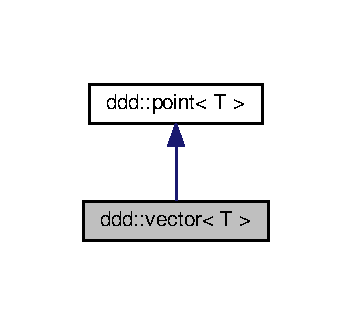
\includegraphics[width=187pt]{d6/df3/classddd_1_1vector__inherit__graph}
\end{center}
\end{figure}


Collaboration diagram for ddd\+:\+:vector$<$ T $>$\+:\nopagebreak
\begin{figure}[H]
\begin{center}
\leavevmode
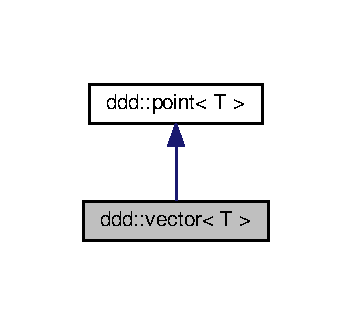
\includegraphics[width=187pt]{d3/d01/classddd_1_1vector__coll__graph}
\end{center}
\end{figure}
\subsection*{Public Member Functions}
\begin{DoxyCompactItemize}
\item 
\mbox{\Hypertarget{classddd_1_1vector_aa318607b6bdd556e5aa371488b3b2da8}\label{classddd_1_1vector_aa318607b6bdd556e5aa371488b3b2da8}} 
\hyperlink{classddd_1_1vector_aa318607b6bdd556e5aa371488b3b2da8}{$\sim$vector} ()
\begin{DoxyCompactList}\small\item\em Class destructor. \end{DoxyCompactList}\item 
\mbox{\Hypertarget{classddd_1_1vector_a9e10641f3e361c24f5a9756bbd1b2d44}\label{classddd_1_1vector_a9e10641f3e361c24f5a9756bbd1b2d44}} 
\hyperlink{classddd_1_1vector_a9e10641f3e361c24f5a9756bbd1b2d44}{vector} (const \hyperlink{classddd_1_1vector}{vector}$<$ T $>$ \&)=default
\begin{DoxyCompactList}\small\item\em Copy constructor. \end{DoxyCompactList}\item 
\mbox{\Hypertarget{classddd_1_1vector_a5231808b18bae0590e5083ff27b29056}\label{classddd_1_1vector_a5231808b18bae0590e5083ff27b29056}} 
\hyperlink{classddd_1_1vector_a5231808b18bae0590e5083ff27b29056}{vector} ()
\begin{DoxyCompactList}\small\item\em Class constructor. \end{DoxyCompactList}\item 
\hyperlink{classddd_1_1vector_a5dec8f05a011372b6b2795827607e6b2}{vector} (const Eigen\+::\+Matrix$<$ T, 3, 1 $>$ \&\hyperlink{classddd_1_1row_object_a30e3d89f19ec4001c9e70d0faaa6c579}{data})
\begin{DoxyCompactList}\small\item\em Class constructor. \end{DoxyCompactList}\item 
\hyperlink{classddd_1_1vector_a90f097b576d026cb86b487546b841622}{vector} (const T \&\hyperlink{classddd_1_1row_object_a29439db5bbde399481c341cb66b7973e}{x}, const T \&\hyperlink{classddd_1_1row_object_adac0d72ea44ad43b82f47b7a26010e4e}{y}, const T \&\hyperlink{classddd_1_1row_object_a8d1d3c3217a0ac951f90e39d980faef4}{z})
\begin{DoxyCompactList}\small\item\em Class constructor. \end{DoxyCompactList}\item 
\hyperlink{classddd_1_1vector_a6a9abe67c1ec0259649dc4647614a62c}{vector} (const \hyperlink{classddd_1_1point}{point}$<$ T $>$ \&input)
\begin{DoxyCompactList}\small\item\em Class constructor. \end{DoxyCompactList}\item 
bool \hyperlink{classddd_1_1vector_a5f26a6f471c836b723c94a5f68a3931d}{operator==} (const \hyperlink{classddd_1_1vector}{vector}$<$ T $>$ \&input)
\begin{DoxyCompactList}\small\item\em Check if two vectors are (exactly) equal. \end{DoxyCompactList}\item 
bool \hyperlink{classddd_1_1vector_a83fb6aea4121e7737ab7642aae23e2df}{operator!=} (const \hyperlink{classddd_1_1vector}{vector}$<$ T $>$ \&input)
\begin{DoxyCompactList}\small\item\em Check if two vectors are (exactly) equal. \end{DoxyCompactList}\item 
bool \hyperlink{classddd_1_1vector_a860847a7c7c93e52b4a83af722eb60f7}{is\+\_\+equal} (const \hyperlink{classddd_1_1vector}{vector}$<$ T $>$ \&input) const
\begin{DoxyCompactList}\small\item\em Check if two vectors are (almost) equal. \end{DoxyCompactList}\item 
bool \hyperlink{classddd_1_1vector_a73bf080395fbbdf9642cf5440d699013}{is\+\_\+notequal} (const \hyperlink{classddd_1_1vector}{vector}$<$ T $>$ \&input) const
\begin{DoxyCompactList}\small\item\em Check if two vectors are (almost) N\+OT equal. \end{DoxyCompactList}\item 
\hyperlink{classddd_1_1vector}{vector}$<$ T $>$ \hyperlink{classddd_1_1vector_a03e9624cbd1f3fa29247c1a67a8678d9}{operator+} (const \hyperlink{classddd_1_1vector}{vector}$<$ T $>$ \&input) const
\begin{DoxyCompactList}\small\item\em Addition operator. \end{DoxyCompactList}\item 
\hyperlink{classddd_1_1vector}{vector}$<$ T $>$ \hyperlink{classddd_1_1vector_aa047958a3d0cf3d3ff3d6ff571920ae0}{operator-\/} (const \hyperlink{classddd_1_1vector}{vector}$<$ T $>$ \&input) const
\begin{DoxyCompactList}\small\item\em Subtraction operator. \end{DoxyCompactList}\item 
\hyperlink{classddd_1_1vector}{vector}$<$ T $>$ \hyperlink{classddd_1_1vector_a9ba05f9c13f8d9cd23f5a5657fcfa948}{operator$\ast$} (const T \&input)
\begin{DoxyCompactList}\small\item\em Scalar product operator. \end{DoxyCompactList}\item 
\hyperlink{classddd_1_1vector}{vector}$<$ T $>$ \hyperlink{classddd_1_1vector_a837824860826c44950c2c48d4bd247e3}{operator/} (const T \&input)
\begin{DoxyCompactList}\small\item\em Scalar division operator. \end{DoxyCompactList}\item 
\mbox{\Hypertarget{classddd_1_1vector_a40b593b08a2dd6af92c5c07bb9faa463}\label{classddd_1_1vector_a40b593b08a2dd6af92c5c07bb9faa463}} 
const \hyperlink{classddd_1_1vector}{vector}$<$ T $>$ \hyperlink{classddd_1_1vector_a40b593b08a2dd6af92c5c07bb9faa463}{normalized} () const
\begin{DoxyCompactList}\small\item\em Return normalized vector. \end{DoxyCompactList}\item 
void \hyperlink{classddd_1_1vector_a97eca6a6625002022ab2442b5cbd0462}{add} (const \hyperlink{classddd_1_1vector}{vector}$<$ T $>$ \&input)
\begin{DoxyCompactList}\small\item\em Addition function. \end{DoxyCompactList}\item 
void \hyperlink{classddd_1_1vector_abf367c7da55ad2c770a90a3ed3c01d5a}{subtract} (const \hyperlink{classddd_1_1vector}{vector}$<$ T $>$ \&input)
\begin{DoxyCompactList}\small\item\em Subtraction function. \end{DoxyCompactList}\item 
const \hyperlink{classddd_1_1vector}{vector}$<$ T $>$ \hyperlink{classddd_1_1vector_a61e3ccdb85f4d41c142c80b429808baf}{dot} (const \hyperlink{classddd_1_1vector}{vector}$<$ T $>$ \&input)
\begin{DoxyCompactList}\small\item\em Dot product function. \end{DoxyCompactList}\item 
const \hyperlink{classddd_1_1vector}{vector}$<$ T $>$ \hyperlink{classddd_1_1vector_a27ac4cb7a469642d497cfe070935ab4b}{cross} (const \hyperlink{classddd_1_1vector}{vector}$<$ T $>$ \&input)
\begin{DoxyCompactList}\small\item\em Cross product function. \end{DoxyCompactList}\item 
bool \hyperlink{classddd_1_1vector_ac3fc063a06940c9893579b1f53f1dda0}{is\+\_\+parallel} (const \hyperlink{classddd_1_1vector}{vector}$<$ T $>$ \&input) const
\begin{DoxyCompactList}\small\item\em Check if two vectors are parallel. \end{DoxyCompactList}\item 
bool \hyperlink{classddd_1_1vector_a4d7791d777455365aed4a1476da78d67}{is\+\_\+notparallel} (const \hyperlink{classddd_1_1vector}{vector}$<$ T $>$ \&input) const
\begin{DoxyCompactList}\small\item\em Check if two vectors are N\+OT parallel. \end{DoxyCompactList}\item 
bool \hyperlink{classddd_1_1vector_aa4093c63121a3787e4b43581f23c3e0a}{is\+\_\+orthogonal} (const \hyperlink{classddd_1_1vector}{vector}$<$ T $>$ \&input) const
\begin{DoxyCompactList}\small\item\em Check if two vectors are orthogonal. \end{DoxyCompactList}\item 
bool \hyperlink{classddd_1_1vector_ab08843c258a0e50ff940ece9c03ad774}{is\+\_\+notorthogonal} (const \hyperlink{classddd_1_1vector}{vector}$<$ T $>$ \&input) const
\begin{DoxyCompactList}\small\item\em Check if two vectors are N\+OT orthogonal. \end{DoxyCompactList}\item 
\mbox{\Hypertarget{classddd_1_1vector_a3ad5fe35a6b91b17a45af430a2622380}\label{classddd_1_1vector_a3ad5fe35a6b91b17a45af430a2622380}} 
const \hyperlink{classddd_1_1vector}{vector}$<$ T $>$ \& \hyperlink{classddd_1_1vector_a3ad5fe35a6b91b17a45af430a2622380}{orthogonal\+Vector} (void) const
\begin{DoxyCompactList}\small\item\em Get an arbitrary vector, orthogonal to the current vector. \end{DoxyCompactList}\item 
bool \hyperlink{classddd_1_1vector_a7595b24534ba95d03d9ace253a7c355f}{operator==} (const \hyperlink{classddd_1_1vector}{vector}$<$ T $>$ \&input) const
\begin{DoxyCompactList}\small\item\em Equality comparison operator. \end{DoxyCompactList}\item 
bool \hyperlink{classddd_1_1vector_a8c18336941576daaff53568d424a27bd}{operator!=} (const \hyperlink{classddd_1_1vector}{vector}$<$ T $>$ \&input) const
\begin{DoxyCompactList}\small\item\em Disequality operator. \end{DoxyCompactList}\item 
const T \& \hyperlink{classddd_1_1vector_ad1a37ce1d1c20c227257fd1fd223c3cf}{angle} (const \hyperlink{classddd_1_1vector}{vector}$<$ T $>$ \&input) const
\begin{DoxyCompactList}\small\item\em Angle between two vectors \mbox{[}rad\mbox{]}. \end{DoxyCompactList}\item 
const T \& \hyperlink{classddd_1_1vector_a97a1359914c22ea1e3928f02fc650bac}{angle} (const \hyperlink{classddd_1_1line}{line}$<$ T $>$ \&input) const
\begin{DoxyCompactList}\small\item\em Angle between vector and line \mbox{[}rad\mbox{]}. \end{DoxyCompactList}\item 
const T \& \hyperlink{classddd_1_1vector_a893bfd1b0209a0a7e7630a3ddf38193d}{angle} (const \hyperlink{classddd_1_1ray}{ray}$<$ T $>$ \&input) const
\begin{DoxyCompactList}\small\item\em Angle between vector and ray \mbox{[}rad\mbox{]}. \end{DoxyCompactList}\item 
const T \& \hyperlink{classddd_1_1vector_aa1d50d563f55d5795d565ed70ec5b845}{angle} (const \hyperlink{classddd_1_1segment}{segment}$<$ T $>$ \&input) const
\begin{DoxyCompactList}\small\item\em Angle between vector and segment \mbox{[}rad\mbox{]}. \end{DoxyCompactList}\item 
\mbox{\Hypertarget{classddd_1_1row_object_a1da634f01207c96a25d5d53a74619afe}\label{classddd_1_1row_object_a1da634f01207c96a25d5d53a74619afe}} 
void \hyperlink{classddd_1_1row_object_a1da634f01207c96a25d5d53a74619afe}{clear} ()
\begin{DoxyCompactList}\small\item\em Clear data. \end{DoxyCompactList}\item 
void \hyperlink{classddd_1_1row_object_a6c87f5fadb3b725f6c52cb08aed98eb2}{scale} (const T \&value)
\begin{DoxyCompactList}\small\item\em Scale object. \end{DoxyCompactList}\item 
T \& \hyperlink{classddd_1_1row_object_aff4fdb32f8b837e224b26de2bcecc7d2}{operator\mbox{[}$\,$\mbox{]}} (const std\+::size\+\_\+t \&i)
\begin{DoxyCompactList}\small\item\em Indexing operator. \end{DoxyCompactList}\item 
const T \& \hyperlink{classddd_1_1row_object_a60418f8af09e6913d16b48f2cb53e826}{operator\mbox{[}$\,$\mbox{]}} (const std\+::size\+\_\+t \&i) const
\begin{DoxyCompactList}\small\item\em Indexing operator. \end{DoxyCompactList}\item 
\mbox{\Hypertarget{classddd_1_1row_object_a29439db5bbde399481c341cb66b7973e}\label{classddd_1_1row_object_a29439db5bbde399481c341cb66b7973e}} 
const T \& \hyperlink{classddd_1_1row_object_a29439db5bbde399481c341cb66b7973e}{x} (void) const
\begin{DoxyCompactList}\small\item\em Get x coordinate. \end{DoxyCompactList}\item 
void \hyperlink{classddd_1_1row_object_afe92fca2bf490cdef9b684bd3847d7eb}{x} (const T \&input)
\begin{DoxyCompactList}\small\item\em Set x coordinate. \end{DoxyCompactList}\item 
\mbox{\Hypertarget{classddd_1_1row_object_adac0d72ea44ad43b82f47b7a26010e4e}\label{classddd_1_1row_object_adac0d72ea44ad43b82f47b7a26010e4e}} 
const T \& \hyperlink{classddd_1_1row_object_adac0d72ea44ad43b82f47b7a26010e4e}{y} (void) const
\begin{DoxyCompactList}\small\item\em Get y coordinate. \end{DoxyCompactList}\item 
void \hyperlink{classddd_1_1row_object_aeb7d81b5fcffd7d8a17fea5b85c37b43}{y} (const T \&input)
\begin{DoxyCompactList}\small\item\em Set y coordinate. \end{DoxyCompactList}\item 
\mbox{\Hypertarget{classddd_1_1row_object_a8d1d3c3217a0ac951f90e39d980faef4}\label{classddd_1_1row_object_a8d1d3c3217a0ac951f90e39d980faef4}} 
const T \& \hyperlink{classddd_1_1row_object_a8d1d3c3217a0ac951f90e39d980faef4}{z} (void) const
\begin{DoxyCompactList}\small\item\em Get z coordinate. \end{DoxyCompactList}\item 
void \hyperlink{classddd_1_1row_object_a42c5766595f9ccb58435d97b8a9e0612}{z} (const T \&input)
\begin{DoxyCompactList}\small\item\em Set z coordinate. \end{DoxyCompactList}\item 
\mbox{\Hypertarget{classddd_1_1row_object_a30e3d89f19ec4001c9e70d0faaa6c579}\label{classddd_1_1row_object_a30e3d89f19ec4001c9e70d0faaa6c579}} 
const Eigen\+::\+Matrix$<$ T, 3, 1 $>$ \& \hyperlink{classddd_1_1row_object_a30e3d89f19ec4001c9e70d0faaa6c579}{data} (void) const
\begin{DoxyCompactList}\small\item\em Get data. \end{DoxyCompactList}\item 
void \hyperlink{classddd_1_1row_object_ae90cbcdfbe32788d18f051a78f8188a6}{data} (const Eigen\+::\+Matrix$<$ T, 3, 1 $>$ \&data)
\begin{DoxyCompactList}\small\item\em Set data. \end{DoxyCompactList}\item 
\mbox{\Hypertarget{classddd_1_1row_object_a760b84053c4b923e060dae45a9284856}\label{classddd_1_1row_object_a760b84053c4b923e060dae45a9284856}} 
const \hyperlink{classddd_1_1point}{point}$<$ T $>$ \hyperlink{classddd_1_1row_object_a760b84053c4b923e060dae45a9284856}{to\+Point} (void)
\begin{DoxyCompactList}\small\item\em Convert to point. \end{DoxyCompactList}\item 
\mbox{\Hypertarget{classddd_1_1row_object_a59fbb28dfc75528f20a0032f6a7bdccd}\label{classddd_1_1row_object_a59fbb28dfc75528f20a0032f6a7bdccd}} 
const \hyperlink{classddd_1_1vector}{vector}$<$ T $>$ \hyperlink{classddd_1_1row_object_a59fbb28dfc75528f20a0032f6a7bdccd}{to\+Vector} (void)
\begin{DoxyCompactList}\small\item\em Convert to vector. \end{DoxyCompactList}\item 
\mbox{\Hypertarget{classddd_1_1row_object_ad567bf2ca914b05a544b73bcec70cc57}\label{classddd_1_1row_object_ad567bf2ca914b05a544b73bcec70cc57}} 
void \hyperlink{classddd_1_1row_object_ad567bf2ca914b05a544b73bcec70cc57}{normalize} ()
\begin{DoxyCompactList}\small\item\em Normalize \hyperlink{classddd_1_1row_object}{row\+Object}. \end{DoxyCompactList}\end{DoxyCompactItemize}


\subsection{Detailed Description}
\subsubsection*{template$<$typename T = Float$>$\newline
class ddd\+::vector$<$ T $>$}

Vector class container. 

Class representing a vector in 3D space. It is constructed by a 3 by 1 Eigen matrix. 

\subsection{Constructor \& Destructor Documentation}
\mbox{\Hypertarget{classddd_1_1vector_a5dec8f05a011372b6b2795827607e6b2}\label{classddd_1_1vector_a5dec8f05a011372b6b2795827607e6b2}} 
\index{ddd\+::vector@{ddd\+::vector}!vector@{vector}}
\index{vector@{vector}!ddd\+::vector@{ddd\+::vector}}
\subsubsection{\texorpdfstring{vector()}{vector()}\hspace{0.1cm}{\footnotesize\ttfamily [1/3]}}
{\footnotesize\ttfamily template$<$typename T = Float$>$ \\
\hyperlink{classddd_1_1vector}{ddd\+::vector}$<$ T $>$\+::\hyperlink{classddd_1_1vector}{vector} (\begin{DoxyParamCaption}\item[{const Eigen\+::\+Matrix$<$ T, 3, 1 $>$ \&}]{data }\end{DoxyParamCaption})\hspace{0.3cm}{\ttfamily [inline]}}



Class constructor. 


\begin{DoxyParams}{Parameters}
{\em data} & Input data \\
\hline
\end{DoxyParams}
\mbox{\Hypertarget{classddd_1_1vector_a90f097b576d026cb86b487546b841622}\label{classddd_1_1vector_a90f097b576d026cb86b487546b841622}} 
\index{ddd\+::vector@{ddd\+::vector}!vector@{vector}}
\index{vector@{vector}!ddd\+::vector@{ddd\+::vector}}
\subsubsection{\texorpdfstring{vector()}{vector()}\hspace{0.1cm}{\footnotesize\ttfamily [2/3]}}
{\footnotesize\ttfamily template$<$typename T = Float$>$ \\
\hyperlink{classddd_1_1vector}{ddd\+::vector}$<$ T $>$\+::\hyperlink{classddd_1_1vector}{vector} (\begin{DoxyParamCaption}\item[{const T \&}]{x,  }\item[{const T \&}]{y,  }\item[{const T \&}]{z }\end{DoxyParamCaption})\hspace{0.3cm}{\ttfamily [inline]}}



Class constructor. 


\begin{DoxyParams}{Parameters}
{\em x} & Input x vector value \\
\hline
{\em y} & Input y vector value \\
\hline
{\em z} & Input z vector value \\
\hline
\end{DoxyParams}
\mbox{\Hypertarget{classddd_1_1vector_a6a9abe67c1ec0259649dc4647614a62c}\label{classddd_1_1vector_a6a9abe67c1ec0259649dc4647614a62c}} 
\index{ddd\+::vector@{ddd\+::vector}!vector@{vector}}
\index{vector@{vector}!ddd\+::vector@{ddd\+::vector}}
\subsubsection{\texorpdfstring{vector()}{vector()}\hspace{0.1cm}{\footnotesize\ttfamily [3/3]}}
{\footnotesize\ttfamily template$<$typename T = Float$>$ \\
\hyperlink{classddd_1_1vector}{ddd\+::vector}$<$ T $>$\+::\hyperlink{classddd_1_1vector}{vector} (\begin{DoxyParamCaption}\item[{const \hyperlink{classddd_1_1point}{point}$<$ T $>$ \&}]{input }\end{DoxyParamCaption})\hspace{0.3cm}{\ttfamily [inline]}}



Class constructor. 


\begin{DoxyParams}{Parameters}
{\em input} & Input point \\
\hline
\end{DoxyParams}


\subsection{Member Function Documentation}
\mbox{\Hypertarget{classddd_1_1vector_a97eca6a6625002022ab2442b5cbd0462}\label{classddd_1_1vector_a97eca6a6625002022ab2442b5cbd0462}} 
\index{ddd\+::vector@{ddd\+::vector}!add@{add}}
\index{add@{add}!ddd\+::vector@{ddd\+::vector}}
\subsubsection{\texorpdfstring{add()}{add()}}
{\footnotesize\ttfamily template$<$typename T = Float$>$ \\
void \hyperlink{classddd_1_1vector}{ddd\+::vector}$<$ T $>$\+::add (\begin{DoxyParamCaption}\item[{const \hyperlink{classddd_1_1vector}{vector}$<$ T $>$ \&}]{input }\end{DoxyParamCaption})\hspace{0.3cm}{\ttfamily [inline]}}



Addition function. 


\begin{DoxyParams}{Parameters}
{\em input} & Input vector object \\
\hline
\end{DoxyParams}
\mbox{\Hypertarget{classddd_1_1vector_ad1a37ce1d1c20c227257fd1fd223c3cf}\label{classddd_1_1vector_ad1a37ce1d1c20c227257fd1fd223c3cf}} 
\index{ddd\+::vector@{ddd\+::vector}!angle@{angle}}
\index{angle@{angle}!ddd\+::vector@{ddd\+::vector}}
\subsubsection{\texorpdfstring{angle()}{angle()}\hspace{0.1cm}{\footnotesize\ttfamily [1/4]}}
{\footnotesize\ttfamily template$<$typename T = Float$>$ \\
const T\& \hyperlink{classddd_1_1vector}{ddd\+::vector}$<$ T $>$\+::angle (\begin{DoxyParamCaption}\item[{const \hyperlink{classddd_1_1vector}{vector}$<$ T $>$ \&}]{input }\end{DoxyParamCaption}) const\hspace{0.3cm}{\ttfamily [inline]}}



Angle between two vectors \mbox{[}rad\mbox{]}. 


\begin{DoxyParams}{Parameters}
{\em input} & Input vector object \\
\hline
\end{DoxyParams}
\mbox{\Hypertarget{classddd_1_1vector_a97a1359914c22ea1e3928f02fc650bac}\label{classddd_1_1vector_a97a1359914c22ea1e3928f02fc650bac}} 
\index{ddd\+::vector@{ddd\+::vector}!angle@{angle}}
\index{angle@{angle}!ddd\+::vector@{ddd\+::vector}}
\subsubsection{\texorpdfstring{angle()}{angle()}\hspace{0.1cm}{\footnotesize\ttfamily [2/4]}}
{\footnotesize\ttfamily template$<$typename T = Float$>$ \\
const T\& \hyperlink{classddd_1_1vector}{ddd\+::vector}$<$ T $>$\+::angle (\begin{DoxyParamCaption}\item[{const \hyperlink{classddd_1_1line}{line}$<$ T $>$ \&}]{input }\end{DoxyParamCaption}) const\hspace{0.3cm}{\ttfamily [inline]}}



Angle between vector and line \mbox{[}rad\mbox{]}. 


\begin{DoxyParams}{Parameters}
{\em input} & Input line object \\
\hline
\end{DoxyParams}
\mbox{\Hypertarget{classddd_1_1vector_a893bfd1b0209a0a7e7630a3ddf38193d}\label{classddd_1_1vector_a893bfd1b0209a0a7e7630a3ddf38193d}} 
\index{ddd\+::vector@{ddd\+::vector}!angle@{angle}}
\index{angle@{angle}!ddd\+::vector@{ddd\+::vector}}
\subsubsection{\texorpdfstring{angle()}{angle()}\hspace{0.1cm}{\footnotesize\ttfamily [3/4]}}
{\footnotesize\ttfamily template$<$typename T = Float$>$ \\
const T\& \hyperlink{classddd_1_1vector}{ddd\+::vector}$<$ T $>$\+::angle (\begin{DoxyParamCaption}\item[{const \hyperlink{classddd_1_1ray}{ray}$<$ T $>$ \&}]{input }\end{DoxyParamCaption}) const\hspace{0.3cm}{\ttfamily [inline]}}



Angle between vector and ray \mbox{[}rad\mbox{]}. 


\begin{DoxyParams}{Parameters}
{\em input} & Input vector object \\
\hline
\end{DoxyParams}
\mbox{\Hypertarget{classddd_1_1vector_aa1d50d563f55d5795d565ed70ec5b845}\label{classddd_1_1vector_aa1d50d563f55d5795d565ed70ec5b845}} 
\index{ddd\+::vector@{ddd\+::vector}!angle@{angle}}
\index{angle@{angle}!ddd\+::vector@{ddd\+::vector}}
\subsubsection{\texorpdfstring{angle()}{angle()}\hspace{0.1cm}{\footnotesize\ttfamily [4/4]}}
{\footnotesize\ttfamily template$<$typename T = Float$>$ \\
const T\& \hyperlink{classddd_1_1vector}{ddd\+::vector}$<$ T $>$\+::angle (\begin{DoxyParamCaption}\item[{const \hyperlink{classddd_1_1segment}{segment}$<$ T $>$ \&}]{input }\end{DoxyParamCaption}) const\hspace{0.3cm}{\ttfamily [inline]}}



Angle between vector and segment \mbox{[}rad\mbox{]}. 


\begin{DoxyParams}{Parameters}
{\em input} & Input vector object \\
\hline
\end{DoxyParams}
\mbox{\Hypertarget{classddd_1_1vector_a27ac4cb7a469642d497cfe070935ab4b}\label{classddd_1_1vector_a27ac4cb7a469642d497cfe070935ab4b}} 
\index{ddd\+::vector@{ddd\+::vector}!cross@{cross}}
\index{cross@{cross}!ddd\+::vector@{ddd\+::vector}}
\subsubsection{\texorpdfstring{cross()}{cross()}}
{\footnotesize\ttfamily template$<$typename T = Float$>$ \\
const \hyperlink{classddd_1_1vector}{vector}$<$T$>$ \hyperlink{classddd_1_1vector}{ddd\+::vector}$<$ T $>$\+::cross (\begin{DoxyParamCaption}\item[{const \hyperlink{classddd_1_1vector}{vector}$<$ T $>$ \&}]{input }\end{DoxyParamCaption})\hspace{0.3cm}{\ttfamily [inline]}}



Cross product function. 


\begin{DoxyParams}{Parameters}
{\em input} & Input vector object \\
\hline
\end{DoxyParams}
\mbox{\Hypertarget{classddd_1_1row_object_ae90cbcdfbe32788d18f051a78f8188a6}\label{classddd_1_1row_object_ae90cbcdfbe32788d18f051a78f8188a6}} 
\index{ddd\+::vector@{ddd\+::vector}!data@{data}}
\index{data@{data}!ddd\+::vector@{ddd\+::vector}}
\subsubsection{\texorpdfstring{data()}{data()}}
{\footnotesize\ttfamily template$<$typename T  = Float$>$ \\
void \hyperlink{classddd_1_1row_object}{ddd\+::row\+Object}$<$ T $>$\+::data (\begin{DoxyParamCaption}\item[{const Eigen\+::\+Matrix$<$ T, 3, 1 $>$ \&}]{data }\end{DoxyParamCaption})\hspace{0.3cm}{\ttfamily [inline]}, {\ttfamily [inherited]}}



Set data. 


\begin{DoxyParams}{Parameters}
{\em data} & Input data \\
\hline
\end{DoxyParams}
\mbox{\Hypertarget{classddd_1_1vector_a61e3ccdb85f4d41c142c80b429808baf}\label{classddd_1_1vector_a61e3ccdb85f4d41c142c80b429808baf}} 
\index{ddd\+::vector@{ddd\+::vector}!dot@{dot}}
\index{dot@{dot}!ddd\+::vector@{ddd\+::vector}}
\subsubsection{\texorpdfstring{dot()}{dot()}}
{\footnotesize\ttfamily template$<$typename T = Float$>$ \\
const \hyperlink{classddd_1_1vector}{vector}$<$T$>$ \hyperlink{classddd_1_1vector}{ddd\+::vector}$<$ T $>$\+::dot (\begin{DoxyParamCaption}\item[{const \hyperlink{classddd_1_1vector}{vector}$<$ T $>$ \&}]{input }\end{DoxyParamCaption})\hspace{0.3cm}{\ttfamily [inline]}}



Dot product function. 


\begin{DoxyParams}{Parameters}
{\em input} & Input vector object \\
\hline
\end{DoxyParams}
\mbox{\Hypertarget{classddd_1_1vector_a860847a7c7c93e52b4a83af722eb60f7}\label{classddd_1_1vector_a860847a7c7c93e52b4a83af722eb60f7}} 
\index{ddd\+::vector@{ddd\+::vector}!is\+\_\+equal@{is\+\_\+equal}}
\index{is\+\_\+equal@{is\+\_\+equal}!ddd\+::vector@{ddd\+::vector}}
\subsubsection{\texorpdfstring{is\+\_\+equal()}{is\_equal()}}
{\footnotesize\ttfamily template$<$typename T = Float$>$ \\
bool \hyperlink{classddd_1_1vector}{ddd\+::vector}$<$ T $>$\+::is\+\_\+equal (\begin{DoxyParamCaption}\item[{const \hyperlink{classddd_1_1vector}{vector}$<$ T $>$ \&}]{input }\end{DoxyParamCaption}) const\hspace{0.3cm}{\ttfamily [inline]}}



Check if two vectors are (almost) equal. 


\begin{DoxyParams}{Parameters}
{\em input} & Input vector object \\
\hline
\end{DoxyParams}
\mbox{\Hypertarget{classddd_1_1vector_a73bf080395fbbdf9642cf5440d699013}\label{classddd_1_1vector_a73bf080395fbbdf9642cf5440d699013}} 
\index{ddd\+::vector@{ddd\+::vector}!is\+\_\+notequal@{is\+\_\+notequal}}
\index{is\+\_\+notequal@{is\+\_\+notequal}!ddd\+::vector@{ddd\+::vector}}
\subsubsection{\texorpdfstring{is\+\_\+notequal()}{is\_notequal()}}
{\footnotesize\ttfamily template$<$typename T = Float$>$ \\
bool \hyperlink{classddd_1_1vector}{ddd\+::vector}$<$ T $>$\+::is\+\_\+notequal (\begin{DoxyParamCaption}\item[{const \hyperlink{classddd_1_1vector}{vector}$<$ T $>$ \&}]{input }\end{DoxyParamCaption}) const\hspace{0.3cm}{\ttfamily [inline]}}



Check if two vectors are (almost) N\+OT equal. 


\begin{DoxyParams}{Parameters}
{\em input} & Input vector object \\
\hline
\end{DoxyParams}
\mbox{\Hypertarget{classddd_1_1vector_ab08843c258a0e50ff940ece9c03ad774}\label{classddd_1_1vector_ab08843c258a0e50ff940ece9c03ad774}} 
\index{ddd\+::vector@{ddd\+::vector}!is\+\_\+notorthogonal@{is\+\_\+notorthogonal}}
\index{is\+\_\+notorthogonal@{is\+\_\+notorthogonal}!ddd\+::vector@{ddd\+::vector}}
\subsubsection{\texorpdfstring{is\+\_\+notorthogonal()}{is\_notorthogonal()}}
{\footnotesize\ttfamily template$<$typename T = Float$>$ \\
bool \hyperlink{classddd_1_1vector}{ddd\+::vector}$<$ T $>$\+::is\+\_\+notorthogonal (\begin{DoxyParamCaption}\item[{const \hyperlink{classddd_1_1vector}{vector}$<$ T $>$ \&}]{input }\end{DoxyParamCaption}) const\hspace{0.3cm}{\ttfamily [inline]}}



Check if two vectors are N\+OT orthogonal. 


\begin{DoxyParams}{Parameters}
{\em input} & Input vector object \\
\hline
\end{DoxyParams}
\mbox{\Hypertarget{classddd_1_1vector_a4d7791d777455365aed4a1476da78d67}\label{classddd_1_1vector_a4d7791d777455365aed4a1476da78d67}} 
\index{ddd\+::vector@{ddd\+::vector}!is\+\_\+notparallel@{is\+\_\+notparallel}}
\index{is\+\_\+notparallel@{is\+\_\+notparallel}!ddd\+::vector@{ddd\+::vector}}
\subsubsection{\texorpdfstring{is\+\_\+notparallel()}{is\_notparallel()}}
{\footnotesize\ttfamily template$<$typename T = Float$>$ \\
bool \hyperlink{classddd_1_1vector}{ddd\+::vector}$<$ T $>$\+::is\+\_\+notparallel (\begin{DoxyParamCaption}\item[{const \hyperlink{classddd_1_1vector}{vector}$<$ T $>$ \&}]{input }\end{DoxyParamCaption}) const\hspace{0.3cm}{\ttfamily [inline]}}



Check if two vectors are N\+OT parallel. 


\begin{DoxyParams}{Parameters}
{\em input} & Input vector object \\
\hline
\end{DoxyParams}
\mbox{\Hypertarget{classddd_1_1vector_aa4093c63121a3787e4b43581f23c3e0a}\label{classddd_1_1vector_aa4093c63121a3787e4b43581f23c3e0a}} 
\index{ddd\+::vector@{ddd\+::vector}!is\+\_\+orthogonal@{is\+\_\+orthogonal}}
\index{is\+\_\+orthogonal@{is\+\_\+orthogonal}!ddd\+::vector@{ddd\+::vector}}
\subsubsection{\texorpdfstring{is\+\_\+orthogonal()}{is\_orthogonal()}}
{\footnotesize\ttfamily template$<$typename T = Float$>$ \\
bool \hyperlink{classddd_1_1vector}{ddd\+::vector}$<$ T $>$\+::is\+\_\+orthogonal (\begin{DoxyParamCaption}\item[{const \hyperlink{classddd_1_1vector}{vector}$<$ T $>$ \&}]{input }\end{DoxyParamCaption}) const\hspace{0.3cm}{\ttfamily [inline]}}



Check if two vectors are orthogonal. 


\begin{DoxyParams}{Parameters}
{\em input} & Input vector object \\
\hline
\end{DoxyParams}
\mbox{\Hypertarget{classddd_1_1vector_ac3fc063a06940c9893579b1f53f1dda0}\label{classddd_1_1vector_ac3fc063a06940c9893579b1f53f1dda0}} 
\index{ddd\+::vector@{ddd\+::vector}!is\+\_\+parallel@{is\+\_\+parallel}}
\index{is\+\_\+parallel@{is\+\_\+parallel}!ddd\+::vector@{ddd\+::vector}}
\subsubsection{\texorpdfstring{is\+\_\+parallel()}{is\_parallel()}}
{\footnotesize\ttfamily template$<$typename T = Float$>$ \\
bool \hyperlink{classddd_1_1vector}{ddd\+::vector}$<$ T $>$\+::is\+\_\+parallel (\begin{DoxyParamCaption}\item[{const \hyperlink{classddd_1_1vector}{vector}$<$ T $>$ \&}]{input }\end{DoxyParamCaption}) const\hspace{0.3cm}{\ttfamily [inline]}}



Check if two vectors are parallel. 


\begin{DoxyParams}{Parameters}
{\em input} & Input vector object \\
\hline
\end{DoxyParams}
\mbox{\Hypertarget{classddd_1_1vector_a83fb6aea4121e7737ab7642aae23e2df}\label{classddd_1_1vector_a83fb6aea4121e7737ab7642aae23e2df}} 
\index{ddd\+::vector@{ddd\+::vector}!operator"!=@{operator"!=}}
\index{operator"!=@{operator"!=}!ddd\+::vector@{ddd\+::vector}}
\subsubsection{\texorpdfstring{operator"!=()}{operator!=()}\hspace{0.1cm}{\footnotesize\ttfamily [1/2]}}
{\footnotesize\ttfamily template$<$typename T = Float$>$ \\
bool \hyperlink{classddd_1_1vector}{ddd\+::vector}$<$ T $>$\+::operator!= (\begin{DoxyParamCaption}\item[{const \hyperlink{classddd_1_1vector}{vector}$<$ T $>$ \&}]{input }\end{DoxyParamCaption})\hspace{0.3cm}{\ttfamily [inline]}}



Check if two vectors are (exactly) equal. 


\begin{DoxyParams}{Parameters}
{\em input} & Input object \\
\hline
\end{DoxyParams}
\mbox{\Hypertarget{classddd_1_1vector_a8c18336941576daaff53568d424a27bd}\label{classddd_1_1vector_a8c18336941576daaff53568d424a27bd}} 
\index{ddd\+::vector@{ddd\+::vector}!operator"!=@{operator"!=}}
\index{operator"!=@{operator"!=}!ddd\+::vector@{ddd\+::vector}}
\subsubsection{\texorpdfstring{operator"!=()}{operator!=()}\hspace{0.1cm}{\footnotesize\ttfamily [2/2]}}
{\footnotesize\ttfamily template$<$typename T = Float$>$ \\
bool \hyperlink{classddd_1_1vector}{ddd\+::vector}$<$ T $>$\+::operator!= (\begin{DoxyParamCaption}\item[{const \hyperlink{classddd_1_1vector}{vector}$<$ T $>$ \&}]{input }\end{DoxyParamCaption}) const\hspace{0.3cm}{\ttfamily [inline]}}



Disequality operator. 


\begin{DoxyParams}{Parameters}
{\em input} & Input vector object \\
\hline
\end{DoxyParams}
\mbox{\Hypertarget{classddd_1_1vector_a9ba05f9c13f8d9cd23f5a5657fcfa948}\label{classddd_1_1vector_a9ba05f9c13f8d9cd23f5a5657fcfa948}} 
\index{ddd\+::vector@{ddd\+::vector}!operator$\ast$@{operator$\ast$}}
\index{operator$\ast$@{operator$\ast$}!ddd\+::vector@{ddd\+::vector}}
\subsubsection{\texorpdfstring{operator$\ast$()}{operator*()}}
{\footnotesize\ttfamily template$<$typename T = Float$>$ \\
\hyperlink{classddd_1_1vector}{vector}$<$T$>$ \hyperlink{classddd_1_1vector}{ddd\+::vector}$<$ T $>$\+::operator$\ast$ (\begin{DoxyParamCaption}\item[{const T \&}]{input }\end{DoxyParamCaption})\hspace{0.3cm}{\ttfamily [inline]}}



Scalar product operator. 


\begin{DoxyParams}{Parameters}
{\em input} & Input scalar \\
\hline
\end{DoxyParams}
\mbox{\Hypertarget{classddd_1_1vector_a03e9624cbd1f3fa29247c1a67a8678d9}\label{classddd_1_1vector_a03e9624cbd1f3fa29247c1a67a8678d9}} 
\index{ddd\+::vector@{ddd\+::vector}!operator+@{operator+}}
\index{operator+@{operator+}!ddd\+::vector@{ddd\+::vector}}
\subsubsection{\texorpdfstring{operator+()}{operator+()}}
{\footnotesize\ttfamily template$<$typename T = Float$>$ \\
\hyperlink{classddd_1_1vector}{vector}$<$T$>$ \hyperlink{classddd_1_1vector}{ddd\+::vector}$<$ T $>$\+::operator+ (\begin{DoxyParamCaption}\item[{const \hyperlink{classddd_1_1vector}{vector}$<$ T $>$ \&}]{input }\end{DoxyParamCaption}) const\hspace{0.3cm}{\ttfamily [inline]}}



Addition operator. 


\begin{DoxyParams}{Parameters}
{\em input} & Input object \\
\hline
\end{DoxyParams}
\mbox{\Hypertarget{classddd_1_1vector_aa047958a3d0cf3d3ff3d6ff571920ae0}\label{classddd_1_1vector_aa047958a3d0cf3d3ff3d6ff571920ae0}} 
\index{ddd\+::vector@{ddd\+::vector}!operator-\/@{operator-\/}}
\index{operator-\/@{operator-\/}!ddd\+::vector@{ddd\+::vector}}
\subsubsection{\texorpdfstring{operator-\/()}{operator-()}}
{\footnotesize\ttfamily template$<$typename T = Float$>$ \\
\hyperlink{classddd_1_1vector}{vector}$<$T$>$ \hyperlink{classddd_1_1vector}{ddd\+::vector}$<$ T $>$\+::operator-\/ (\begin{DoxyParamCaption}\item[{const \hyperlink{classddd_1_1vector}{vector}$<$ T $>$ \&}]{input }\end{DoxyParamCaption}) const\hspace{0.3cm}{\ttfamily [inline]}}



Subtraction operator. 


\begin{DoxyParams}{Parameters}
{\em input} & Input object \\
\hline
\end{DoxyParams}
\mbox{\Hypertarget{classddd_1_1vector_a837824860826c44950c2c48d4bd247e3}\label{classddd_1_1vector_a837824860826c44950c2c48d4bd247e3}} 
\index{ddd\+::vector@{ddd\+::vector}!operator/@{operator/}}
\index{operator/@{operator/}!ddd\+::vector@{ddd\+::vector}}
\subsubsection{\texorpdfstring{operator/()}{operator/()}}
{\footnotesize\ttfamily template$<$typename T = Float$>$ \\
\hyperlink{classddd_1_1vector}{vector}$<$T$>$ \hyperlink{classddd_1_1vector}{ddd\+::vector}$<$ T $>$\+::operator/ (\begin{DoxyParamCaption}\item[{const T \&}]{input }\end{DoxyParamCaption})\hspace{0.3cm}{\ttfamily [inline]}}



Scalar division operator. 


\begin{DoxyParams}{Parameters}
{\em input} & Input scalar \\
\hline
\end{DoxyParams}
\mbox{\Hypertarget{classddd_1_1vector_a5f26a6f471c836b723c94a5f68a3931d}\label{classddd_1_1vector_a5f26a6f471c836b723c94a5f68a3931d}} 
\index{ddd\+::vector@{ddd\+::vector}!operator==@{operator==}}
\index{operator==@{operator==}!ddd\+::vector@{ddd\+::vector}}
\subsubsection{\texorpdfstring{operator==()}{operator==()}\hspace{0.1cm}{\footnotesize\ttfamily [1/2]}}
{\footnotesize\ttfamily template$<$typename T = Float$>$ \\
bool \hyperlink{classddd_1_1vector}{ddd\+::vector}$<$ T $>$\+::operator== (\begin{DoxyParamCaption}\item[{const \hyperlink{classddd_1_1vector}{vector}$<$ T $>$ \&}]{input }\end{DoxyParamCaption})\hspace{0.3cm}{\ttfamily [inline]}}



Check if two vectors are (exactly) equal. 


\begin{DoxyParams}{Parameters}
{\em input} & Input object \\
\hline
\end{DoxyParams}
\mbox{\Hypertarget{classddd_1_1vector_a7595b24534ba95d03d9ace253a7c355f}\label{classddd_1_1vector_a7595b24534ba95d03d9ace253a7c355f}} 
\index{ddd\+::vector@{ddd\+::vector}!operator==@{operator==}}
\index{operator==@{operator==}!ddd\+::vector@{ddd\+::vector}}
\subsubsection{\texorpdfstring{operator==()}{operator==()}\hspace{0.1cm}{\footnotesize\ttfamily [2/2]}}
{\footnotesize\ttfamily template$<$typename T = Float$>$ \\
bool \hyperlink{classddd_1_1vector}{ddd\+::vector}$<$ T $>$\+::operator== (\begin{DoxyParamCaption}\item[{const \hyperlink{classddd_1_1vector}{vector}$<$ T $>$ \&}]{input }\end{DoxyParamCaption}) const\hspace{0.3cm}{\ttfamily [inline]}}



Equality comparison operator. 


\begin{DoxyParams}{Parameters}
{\em input} & Input vector object \\
\hline
\end{DoxyParams}
\mbox{\Hypertarget{classddd_1_1row_object_aff4fdb32f8b837e224b26de2bcecc7d2}\label{classddd_1_1row_object_aff4fdb32f8b837e224b26de2bcecc7d2}} 
\index{ddd\+::vector@{ddd\+::vector}!operator\mbox{[}\mbox{]}@{operator[]}}
\index{operator\mbox{[}\mbox{]}@{operator[]}!ddd\+::vector@{ddd\+::vector}}
\subsubsection{\texorpdfstring{operator[]()}{operator[]()}\hspace{0.1cm}{\footnotesize\ttfamily [1/2]}}
{\footnotesize\ttfamily template$<$typename T  = Float$>$ \\
T\& \hyperlink{classddd_1_1row_object}{ddd\+::row\+Object}$<$ T $>$\+::operator\mbox{[}$\,$\mbox{]} (\begin{DoxyParamCaption}\item[{const std\+::size\+\_\+t \&}]{i }\end{DoxyParamCaption})\hspace{0.3cm}{\ttfamily [inline]}, {\ttfamily [inherited]}}



Indexing operator. 


\begin{DoxyParams}{Parameters}
{\em i} & Input index \\
\hline
\end{DoxyParams}
\mbox{\Hypertarget{classddd_1_1row_object_a60418f8af09e6913d16b48f2cb53e826}\label{classddd_1_1row_object_a60418f8af09e6913d16b48f2cb53e826}} 
\index{ddd\+::vector@{ddd\+::vector}!operator\mbox{[}\mbox{]}@{operator[]}}
\index{operator\mbox{[}\mbox{]}@{operator[]}!ddd\+::vector@{ddd\+::vector}}
\subsubsection{\texorpdfstring{operator[]()}{operator[]()}\hspace{0.1cm}{\footnotesize\ttfamily [2/2]}}
{\footnotesize\ttfamily template$<$typename T  = Float$>$ \\
const T\& \hyperlink{classddd_1_1row_object}{ddd\+::row\+Object}$<$ T $>$\+::operator\mbox{[}$\,$\mbox{]} (\begin{DoxyParamCaption}\item[{const std\+::size\+\_\+t \&}]{i }\end{DoxyParamCaption}) const\hspace{0.3cm}{\ttfamily [inline]}, {\ttfamily [inherited]}}



Indexing operator. 


\begin{DoxyParams}{Parameters}
{\em i} & Input index \\
\hline
\end{DoxyParams}
\mbox{\Hypertarget{classddd_1_1row_object_a6c87f5fadb3b725f6c52cb08aed98eb2}\label{classddd_1_1row_object_a6c87f5fadb3b725f6c52cb08aed98eb2}} 
\index{ddd\+::vector@{ddd\+::vector}!scale@{scale}}
\index{scale@{scale}!ddd\+::vector@{ddd\+::vector}}
\subsubsection{\texorpdfstring{scale()}{scale()}}
{\footnotesize\ttfamily template$<$typename T  = Float$>$ \\
void \hyperlink{classddd_1_1row_object}{ddd\+::row\+Object}$<$ T $>$\+::scale (\begin{DoxyParamCaption}\item[{const T \&}]{value }\end{DoxyParamCaption})\hspace{0.3cm}{\ttfamily [inline]}, {\ttfamily [inherited]}}



Scale object. 


\begin{DoxyParams}{Parameters}
{\em value} & Scale value \\
\hline
\end{DoxyParams}
\mbox{\Hypertarget{classddd_1_1vector_abf367c7da55ad2c770a90a3ed3c01d5a}\label{classddd_1_1vector_abf367c7da55ad2c770a90a3ed3c01d5a}} 
\index{ddd\+::vector@{ddd\+::vector}!subtract@{subtract}}
\index{subtract@{subtract}!ddd\+::vector@{ddd\+::vector}}
\subsubsection{\texorpdfstring{subtract()}{subtract()}}
{\footnotesize\ttfamily template$<$typename T = Float$>$ \\
void \hyperlink{classddd_1_1vector}{ddd\+::vector}$<$ T $>$\+::subtract (\begin{DoxyParamCaption}\item[{const \hyperlink{classddd_1_1vector}{vector}$<$ T $>$ \&}]{input }\end{DoxyParamCaption})\hspace{0.3cm}{\ttfamily [inline]}}



Subtraction function. 


\begin{DoxyParams}{Parameters}
{\em input} & Input vector object \\
\hline
\end{DoxyParams}
\mbox{\Hypertarget{classddd_1_1row_object_afe92fca2bf490cdef9b684bd3847d7eb}\label{classddd_1_1row_object_afe92fca2bf490cdef9b684bd3847d7eb}} 
\index{ddd\+::vector@{ddd\+::vector}!x@{x}}
\index{x@{x}!ddd\+::vector@{ddd\+::vector}}
\subsubsection{\texorpdfstring{x()}{x()}}
{\footnotesize\ttfamily template$<$typename T  = Float$>$ \\
void \hyperlink{classddd_1_1row_object}{ddd\+::row\+Object}$<$ T $>$\+::x (\begin{DoxyParamCaption}\item[{const T \&}]{input }\end{DoxyParamCaption})\hspace{0.3cm}{\ttfamily [inline]}, {\ttfamily [inherited]}}



Set x coordinate. 


\begin{DoxyParams}{Parameters}
{\em input} & Input value \\
\hline
\end{DoxyParams}
\mbox{\Hypertarget{classddd_1_1row_object_aeb7d81b5fcffd7d8a17fea5b85c37b43}\label{classddd_1_1row_object_aeb7d81b5fcffd7d8a17fea5b85c37b43}} 
\index{ddd\+::vector@{ddd\+::vector}!y@{y}}
\index{y@{y}!ddd\+::vector@{ddd\+::vector}}
\subsubsection{\texorpdfstring{y()}{y()}}
{\footnotesize\ttfamily template$<$typename T  = Float$>$ \\
void \hyperlink{classddd_1_1row_object}{ddd\+::row\+Object}$<$ T $>$\+::y (\begin{DoxyParamCaption}\item[{const T \&}]{input }\end{DoxyParamCaption})\hspace{0.3cm}{\ttfamily [inline]}, {\ttfamily [inherited]}}



Set y coordinate. 


\begin{DoxyParams}{Parameters}
{\em input} & Input value \\
\hline
\end{DoxyParams}
\mbox{\Hypertarget{classddd_1_1row_object_a42c5766595f9ccb58435d97b8a9e0612}\label{classddd_1_1row_object_a42c5766595f9ccb58435d97b8a9e0612}} 
\index{ddd\+::vector@{ddd\+::vector}!z@{z}}
\index{z@{z}!ddd\+::vector@{ddd\+::vector}}
\subsubsection{\texorpdfstring{z()}{z()}}
{\footnotesize\ttfamily template$<$typename T  = Float$>$ \\
void \hyperlink{classddd_1_1row_object}{ddd\+::row\+Object}$<$ T $>$\+::z (\begin{DoxyParamCaption}\item[{const T \&}]{input }\end{DoxyParamCaption})\hspace{0.3cm}{\ttfamily [inline]}, {\ttfamily [inherited]}}



Set z coordinate. 


\begin{DoxyParams}{Parameters}
{\em input} & Input value \\
\hline
\end{DoxyParams}


The documentation for this class was generated from the following files\+:\begin{DoxyCompactItemize}
\item 
src/ddd\+\_\+instantiate.\+hh\item 
src/ddd\+\_\+vector.\+hh\end{DoxyCompactItemize}

%--- End generated contents ---

% Index
\backmatter
\newpage
\phantomsection
\clearemptydoublepage
\addcontentsline{toc}{chapter}{Index}
\printindex

\end{document}
